\documentclass[a4paper,12pt]{report}
\usepackage{amsmath}
\usepackage{graphicx}
\usepackage{datetime2}
\usepackage{url}
\usepackage{amsfonts}
\usepackage{extarrows} 
\usepackage{makecell}
\usepackage{placeins}
\usepackage{fancyhdr}
\usepackage{tikz}
\usepackage{physics}
%\usepackage{mathabx}
\usepackage[]{algorithm2e}
\usepackage[skins]{tcolorbox}
\usepackage{subcaption} 
\usetikzlibrary{positioning,calc}
\usepackage{draftwatermark}
\usepackage{framed}
\SetWatermarkText{DRAFT}
\SetWatermarkScale{5}

\usepackage[left=1in,right=1in,top=1.2in,bottom=1.2in]{geometry}

\newcommand{\tikzmark}[1]{\tikz[overlay,remember picture] \node (#1) [anchor=base] {};}
\newcommand{\snode}[3]{\node [] (#1) at (#2) {$\mathstrut #3$}}
\newcommand{\spath}[2]{\draw[<->] (#1) -- (#2) node [midway, above] () {S}}
\newcommand{\ppath}[2]{\draw[<->] (#1) -- (#2) node [midway, above] () {P}}
 
\fancypagestyle{firstpage}{%
\fancyhf{} % clear all six fields
\renewcommand{\headrulewidth}{0pt}
\renewcommand{\footrulewidth}{0pt}
}
\fancypagestyle{firstcoverpage}{%
\fancyhf{} % clear all six fields
\fancyfoot[C]{\thepage}
\renewcommand{\headrulewidth}{0pt}
\renewcommand{\footrulewidth}{0pt}
}
\fancypagestyle{followingpage}{%
\fancyhf{} % clear all six fields
\fancyhead[LE,RO]{\textbf{\thepage}}
\fancyhead[LO,RE]{\nouppercase{\rightmark}}
\renewcommand{\headrulewidth}{0.7pt}
\renewcommand{\footrulewidth}{0pt}
}
\pagestyle{followingpage}
 

%\documentclass[aip,reprint]{revtex4-1}

\newcommand{\ovl}{\overline}
\newcommand{\unl}{\underline}
\newcommand{\oli}{\overline{i}}
\newcommand{\olj}{\overline{j}}
\newcommand{\olk}{\overline{k}}
\newcommand{\oll}{\overline{l}}
\newcommand{\ola}{\overline{a}}
\newcommand{\olb}{\overline{b}}
\newcommand{\olc}{\overline{c}}
\newcommand{\old}{\overline{d}}

\newcommand{\ooli}{\overline{\overline{i}}}
\newcommand{\oolj}{\overline{\overline{j}}}
\newcommand{\oolk}{\overline{\overline{k}}}
\newcommand{\ooll}{\overline{\overline{l}}}
\newcommand{\oola}{\overline{\overline{a}}}
\newcommand{\oolb}{\overline{\overline{b}}}
\newcommand{\oolc}{\overline{\overline{c}}}
\newcommand{\oold}{\overline{\overline{d}}}

\newcommand{\ool}[1]{\overline{\overline{#1}}}

\newcommand{\eps}{\epsilon}

\newcommand{\olI}{\overline{I}}
\newcommand{\olJ}{\overline{J}}
\newcommand{\olK}{\overline{K}}
\newcommand{\olL}{\overline{L}}
\newcommand{\olA}{\overline{A}}
\newcommand{\olB}{\overline{B}}
\newcommand{\olC}{\overline{C}}
\newcommand{\olD}{\overline{D}}

\newcommand{\doti}{\hat{i}}
\newcommand{\dotj}{\hat{j}}
\newcommand{\dotk}{\hat{k}}
\newcommand{\dotl}{\hat{l}}

\newcommand{\dota}{\hat{a}}
\newcommand{\dotb}{\hat{b}}
\newcommand{\dotc}{\hat{c}}
\newcommand{\dotd}{\hat{d}}

\newcommand{\odota}{\overline{\dota}}
\newcommand{\odotb}{\overline{\dotb}}
\newcommand{\udoti}{\underline{\doti}}
\newcommand{\udotj}{\underline{\dotj}}
\newcommand{\udotk}{\underline{\dotk}}
\newcommand{\odotc}{\overline{\dotc}}

\newcommand{\uli}{\underline{i}}
\newcommand{\ulj}{\underline{j}}
\newcommand{\ulk}{\underline{k}}
\newcommand{\ull}{\underline{l}}
\newcommand{\ulm}{\underline{m}}
\newcommand{\uln}{\underline{n}}

\newcommand{\ulgm}{\underline{\mu}}
\newcommand{\olgm}{\overline{\mu}}
\newcommand{\ulgn}{\underline{\nu}}
\newcommand{\olgn}{\overline{\nu}}
\newcommand{\ulgk}{\underline{\kappa}}
\newcommand{\ulgt}{\underline{\tau}}
\newcommand{\ulgl}{\underline{\lambda}}
\newcommand{\olgl}{\overline{\lambda}} % use for b
\newcommand{\olga}{\overline{\alpha}}
\newcommand{\olgb}{\overline{\beta}}
\newcommand{\olgs}{\overline{\sigma}} % use for a
\newcommand{\olgg}{\overline{\gamma}} 
\newcommand{\olgd}{\overline{\delta}}

\newcommand{\gm}{\mu}
\newcommand{\gn}{\nu}
\newcommand{\gk}{\kappa}
\newcommand{\gl}{\lambda}
\newcommand{\ga}{\alpha}
\newcommand{\gb}{\beta}
\renewcommand{\gg}{\gamma}
\newcommand{\gd}{\delta}
\newcommand{\gs}{\sigma}

\newcommand{\pa}{^{(\alpha)}}
\newcommand{\pt}{^{(\theta)}}
\newcommand{\pdg}{^{\dagger}}
\newcommand{\ptw}{^{(\theta,\omega)}}

\newcommand{\calJ}{\mathcal{J}}
\newcommand{\calK}{\mathcal{K}}
\newcommand{\calZ}{\mathcal{Z}}

\newcommand{\cn}[2]{\left( #1 \mid #2 \right)}
\newcommand{\mbf}[1]{\mathbf{#1}}
\newcommand{\bfun}[2]{\chi_{#1}(\mathbf{r_{#2}})}
\newcommand{\cbra}[1]{\left( #1 \right\rvert }
\newcommand{\cket}[1]{\left\lvert #1 \right)}
\newcommand{\B}[2]{B_{#1}^{#2}}
\newcommand{\x}[2]{_{#1}^{#2}}
\newcommand{\xlr}[1]{\xleftrightarrow{#1}}
\newcommand{\wpa}{\left\lvert w\pa \right\rvert}

\newcommand{\bk}[2]{\bra{#1} \ket{#2}}
\newcommand{\sbk}[2]{\bra{#1} {} \ket{#2}}

\newcommand{\ep}{\epsilon}

\newcommand{\ccpx}[1]{\mathcal{O}(N^{#1})}

\newcommand{\sym}[2]{_{#1 \leftrightarrow #2}}

\newcommand{\ssg}{^{\sigma}}

\newcommand{\mbfx}{\mathbf{x}}

\setcellgapes{10pt}

\newtcolorbox{myframe}[2][]{%
  enhanced,colback=white,colframe=black,coltitle=black,
  sharp corners,boxrule=0.4pt,
  fonttitle=\itshape,
  attach boxed title to bottom right={yshift=0.3\baselineskip+0.4pt,xshift=-2mm},
  boxed title style={tile,size=minimal,left=0.5mm,right=0.5mm,
    colback=white,before upper=\strut},
  title=#2,#1
}

\allowdisplaybreaks 

\newcommand{\forcond}{$\alpha=0$ \KwTo $n_{lap}$}
\newcounter{ISTEP}
\newcommand{\itemR}{\item \refstepcounter{ISTEP}}

\def\signed #1{{\leavevmode\unskip\nobreak\hfil\penalty50\hskip2em
  \hbox{}\nobreak\hfil(#1)%
  \parfillskip=0pt \finalhyphendemerits=0 \endgraf}}

\newsavebox\mybox
\newenvironment{aquote}[1]
  {\savebox\mybox{#1}\begin{quote}}
  {\signed{\usebox\mybox}\end{quote}}

%\newcommand{\nperp}{^{\not\perp}}

\begin{document}

\author{Maximilien Alexandre Ambroise}
\title{The Algebraic Diagrammatic Construction Method For High Performance Computing Environments Using an Atomic Orbital Representation}

\begin{titlepage}
\begin{center}
{\Huge\scshape Inaugural - Dissertation \\}
{ zur Erlangung der Doktorwürde der \\
Naturwissenschaftlich-Mathematischen Gesamtfakultät \\
der Ruprecht-Karls-Universität Heidelberg \\}
\vspace{1cm}
{\huge\bfseries The Algebraic Diagrammatic Construction Method For High Performance Computing Environments \\}
{\Large\bfseries Using an Atomic Orbital Representation \\}
 
%----------------------------------------------------------------
\vspace{1.5cm}
{vorgelegt von\\}
\vspace*{1.5cm}
{\Large Maximilien Alexandre Ambroise}\\
{\large aus Differdingen, Luxemburg}\\
%----------------------------------------------------------------
\vspace{2cm}
{Juli 2021} \\[5pt]
\vspace{2cm}
{\bfseries Gutachter: \\}
{Prof. Dr. Andreas Dreuw \\ ...}\\
\end{center}
\end{titlepage}

\pagenumbering{roman}

\newpage

Licensing

\newpage

\newpage

\noindent {\Large \bfseries Notation for Orbital Representations}

\begin{table}[h]
\setlength{\tabcolsep}{14pt}
\renewcommand{\arraystretch}{1.5}
\begin{tabular}{ll}
$\mu$, $\nu$, $\gamma$, $\lambda$, ... & atomic orbitals \\
$i$, $j$, $k$, $l$, ... & occupied molecular orbitals \\
$a$, $b$, $c$, $d$, ... & virtual molecular orbitals \\
$\uli$, $\ulj$, $\ulk$, $\ull$, ... & local occupied molecular orbitals \\
$\ola$, $\olb$, $\olc$, $\old$, ... & local virtual molecular orbitals \\
$I$, $J$, $K$, $L$, ... & occupied molecular spin orbitals \\
$A$, $B$, $C$, $D$, ... & virtual molecular spin orbitals \\
$\ulgm$, $\ulgn$, $\ulgl$, $\ulgs$, ... & occupied projected atomic orbitals \\
$\olgm$, $\olgn$, $\olgl$, $\olgs$, ... & virtual projected atomic orbitals
\end{tabular}
\end{table}

\noindent {\Large \bfseries Abbreviations}



\newpage

\tableofcontents

\newpage

\listoffigures

\newpage

\listoftables

\newpage

\pagenumbering{arabic}

\chapter*{Introduction}

This is the introduction. Talk about sparsity. Show sparse matrix. How does sparsity arise, what can we do with it, where else does it emerge?
State of arts: adc now, adc in the future

Exact solution: three body problem
Helium: cannot be solved exactly: approximate methods. finite grid, finite basis
solutions
ground state excited state
computational resources

\begin{figure}
\centering
\includegraphics[scale=0.05]{Pics/fock.pdf}
\caption{Adenine-guanine fock matrix Hartree FOck cc-pVTZ}
\label{SparseExample}
\end{figure}

\newpage

\part{}

\chapter{Theory: The Basics}

\section{Ground Work}

\subsection{The Schrödinger Equation}

\subsection{Basis Sets}

\subsection{Electron Integrals}

\section{Hartree Fock}

\section{Post-Hartree Fock Ground State}

\subsection{Configuration Interaction}

\subsection{Perturbation Theory}

\subsection{Coupled Cluster}

\section{Post-Hartree Fock Excited State}

\subsection{Configuration Interaction}

\subsection{Coupled Cluster Linear Repsonse}

\subsection{Equation-of-Motion Coupled Cluster}

\subsection{Algebraic Diagrammatic Construction}


\chapter{Electronic Excited States}

\begin{quote}
  "The XXIst century might be very well the century of light. Understanding and controlling photoexcited systems will be crucial for future research in many branches of optics and photonics."
  \begin{flushright}
    \small{--- \textit{L. González, D. Escudero, L. Serrano-Andrés (2011) \cite{Gon2012} }}
  \end{flushright}
\end{quote}

A quantum system is said to be in an \emph{excited state} if that state is at a higher energy level than the ground state, for example by absorption of one or more light quanta. While computing ground state properties has become routine even for larger molecules, the extension of the standard models to excited state properties is an active field of research. Triggered by the development of complex, high-resolution spectroscopic techniques such as X-ray spectroscopy \cite{Nor2018a}, and advances in photochemistry \cite{Gon2012}, the demand for accurate and computational methods of excited states has been steadily increasing. Electronic spectra are often very difficult to interpret, and \emph{computational spectroscopy} has emerged as an important tool to explain the underlying mechanisms.

Excited states are notoriously difficult to model, and similarly to their ground state analogs, there is no single method to rule them all. Over the years, many different approaches have been proposed, each with their strengths and weaknesses. This section will go over the most popular, single-reference methods  available, with a focus on the algebraic diagrammatic construction method. 

\section{Nature of Excited States}

The potential energy landscape of electronic excited states is complex and governed by various absorption and decay mechanisms. Excitations are generally grouped into three categories:
\begin{enumerate}
\item \emph{Valence excitations}, where valence electrons are excited into (local) higher lying unoccupied orbitals above the Fermi level
\item \emph{Rydberg excitations}, where electrons are excited into very diffuse orbitals around the molecule
\item \emph{Charge transfer excitations} (CT), where electrons are excited to different parts of the molecule or different molecules entirely. 
\end{enumerate}

Excited states typically have lifetimes and decay back to the ground state via several different mechanisms. Figure \ref{fig:PESEX} illustrates the different processes. The notation $S$, $D$, $T$ ... is used to denote singlet, doublet, triplet ... states and the subscripts indicate the energy level, where 0 is the ground state, 1 is the first excited state for the given spin symmetry, 2 is the second excited state etc. The transition from the ground state $S_0$ to the excited state $S_1$ on the same reaction coordinate is known as a \emph{vertical excitation}. The excited state may be in a higher vibrational state at that reaction coordinate (indicated by the lines within the potential wells), and relax to the lowest level. The difference between these two points is known as the \emph{reorganization energy}, and the difference between the lowest vibrational states of $S_0$ and the excited state is known as the \emph{adiabatic excitation} energy. The 
molecule returns to the ground state by emitting a photon in a process known as \emph{fluorescence}. 

Surfaces of different states may cross at specific reaction coordinates. The crossing between states with different multiplicity (e.g. S$_1$ to T$_1$) is known as an inter-system crossing (ISC). The process between two states where the crossing takes place between molecules of the same spin-symmetry is known as \emph{internal conversion} (IC), and takes place at a \emph{conical intersection} (CoIn). The S$_1$ excited state can cross over to the T$_1$ state via an ISC which then decays in a process known as \emph{phosphorescence}, or it can decay radiation-less via the CoIn. At the ISC and CoIn, the Born-Oppenheimer approximation breaks down due to non-adiabatic coupling between electrons and nuclei. ISCs and CoIns are central to describing the dynamics in photochemical events \cite{Mig2008,Mat2011,Kim2015,Zhu2016}.

For the sake of brevity, this chapter will focus on the computational of vertical excitation energies only.

\begin{figure}
\centering
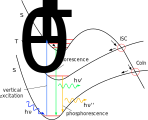
\includegraphics[scale=0.8]{Pics/PESEX}
\caption{Potential energy surface of a chemical system depicting the major pathways encountered in spectroscopy and photochemistry.}
\label{fig:PESEX}
\end{figure}

\section{Explicit Optimization of the Excited State Wave Function}

One of the conceptually simplest approaches for obtaining information on excited states is explicit optimization of the excited wave function. The excitation energy is then directly computed by taking the difference between the ground state energy and the energy of excited state $i$
\begin{equation}
E_{0\rightarrow i} = E_i - E_0 
\end{equation} 
\noindent Any ground state model discussed in the previous chapter can be used. This approach to excited states is known by different names, depending on which approximation is used. Generally, the Greek letter $\Delta$ is just prepended to the method name, giving $\Delta$SCF or $\Delta$HF for Hartree-Fock \cite{Bag1965,Deu1976,Amb2019}, $\Delta$KS (Kohn-Sham) or $\Delta$DFT for DFT \cite{Tri1999,Tak2003,Bes2009}, and so on. At the moment of writing, excitation energies are also routinely computed using $\Delta$MP$n$ \cite{Hol2011}, $\Delta$CI, $\Delta$MCSCF \cite{Sch2015} and $\Delta$CC \cite{Hol2011,Zhe2019}. From here on out, $\Delta$X will be used as an umbrella term to group all aforementioned terms. 

Despite the simplicity of the $\Delta$X methods, obtaining a solution to the KS or HF equations for higher energy states is non-trivial. By the variational principle, the SCF method finds the lowest energy solution. A HF type excited wave function may therefore collapse to that lowest energy solution during the SCF procedure (variational collapse). For small symmetric molecules, it is possible to converge excited states if they have a different spin multiplicity or spatial point group to the ground state. If the ground and excited state have the same symmetry however, this approach will not work. This technical difficulty was one of reasons why $\Delta$X methods never gained much ground compared to more sophisticated methods.

In 2008, Gilbert et al. \cite{Gil2008} proposed a modification the SCF procedure that prevents variational collapse, known as the \emph{maximum overlap method} (MOM). On each iteration, the new guess orbitals are obtained by diagonalization of the Fock matrix which is constructed using the old coefficients
\begin{equation}
\mbf{F}(\mbf{C}^{old})\mbf{C}^{new} = \mbf{S}\mbf{C}^{new}\epsilon
\end{equation}
\noindent At this step, it is possible to decide which of those new orbitals are actually occupied. Normally, the $n_{occ}$ eigenvectors with the lowest eigenvalues are chosen as the new occupied MOs. Alternatively, the MOM protocol chooses the set of new MOs that overlap most with the span of the old coefficients, by evaluating the overlap matrix
\begin{equation}
\mbf{O} = (\mbf{C}^{old})\pdg \mbf{C}
\end{equation}
\noindent The maximum overlap method has led to a renewed interest in the $\Delta$X methods in recent years, especially in the context of core excitations and ionizations. 

Adding to the above-mentioned technical difficulties, there are several other known criticisms. First, each excited state requires a separately optimized wave function, which may become a limiting factor. Second, the $\Delta$X methods assume that a transition can be represented by an excitation involving two orbitals. The separate optimization generally leads to the excited states being non-orthogonal, and there is considerable overlap between high and low energy states \cite{Dav1964,Dav1965,Gil2008}. $\Delta$X is therefore assumed to be only applicable to low-lying excited states. Third, the transition moments cannot be computed directly, but need to be evaluated using Fermi's Golden Rule \cite{Gro2008}. Furthermore, to allow a comparison with experimental XAS spectra, the calculated transition energies must be convoluted, for example by Gaussian functions, to 
account for the finite experimental resolution and  lifetime of the electron hole. Finally, using an unrestricted HF or KS formalism leads to spin contamination. A single excited state is not a pure singlet but a mixture of singlet and triplet state. Spin contamination can be alleviated by applying Ziegler's spin purification formula \cite{Zie1977}:

\begin{equation}
E_S = 2 E_{mixed} - E_T
\end{equation}

Despite these disadvantages, $\Delta$X is still an attractive and low-cost alternative to response and propagator methods.


\section{The Algebraic Diagrammatic Construction Method}

The algebraic diagrammatic construction (ADC) scheme is an excited state method originating from Green's functions \cite{Sch1982,Sch2018}. By diagrammatic perturbation expansion of electron propagators, ADC gives a hierarchy of methods which systematically converge to the exact solution (Full CI).  

\subsection{Many-Body Green's Function}

Many-Body Green's Functions (MBGFs) are powerful tools to treat electron correlation in quantum mechanics. They are more commonly encountered in (condensed matter) physics, for the modeling of strongly correlated systems such as metals or semi-conductors. MBGFs get their name from their building blocks: Green's functions (GFs). GFs, or \emph{correlation functions}, are special solutions to differential equations (DEQs).

Consider the inhomogeneous DEQ in one dimension:
\begin{equation}
\hat{D}_x y(x) = f(x)
\end{equation}
\noindent where $\hat{D}$ is a linear differential operator. The general solution can be divided into a \emph{homogeneous} and a \emph{special} part
\begin{equation}
y(x) = y_{hom}(x) + y_{spec}(x)
\end{equation}
\noindent where $y_{hom}$ is the solution to the homogeneous equation $\hat{D}y_{hom}(x)$ = 0. The special solution can be expressed in terms of GFs which are defined as the solution to the DEQ where the inhomogeneity is a Dirac function:
\begin{equation}
\hat{D}_x G(x,x') = \delta(x-x')
\end{equation}
\noindent A special solution can then be constructed by
\begin{equation}
y_{spec} = \int G(x,x')f(x') dx
\end{equation}
\noindent for any inhomogeneity $f(x)$. 

The Schrödinger equation is also a differential equation where the inhomogeneity takes the role of the external perturbation $V$
\begin{equation}
\left[ i\frac{\partial}{\partial t} + \frac{1}{2} \nabla^2 \right] \Psi(\mbf{r},t) = V(\mbf{r},t) \Psi(\mbf{r},t)
\end{equation}
\noindent The wave function may then be expressed by
\begin{equation}
\Psi(\mbf{r},t) = \int G(\mbf{r},t;\mbf{r}',t') \Psi
\end{equation}
\noindent The GF has the effect of \emph{propagating} the wave function from a given time and position to another time and space coordinate. GFs are therefore also known as \emph{propagators}.

The MBGFs form a hierarchy, in which the one-particle GFs are the lowest rank (Figure \ref{fig:PROP}). One-particle GFs can be used to extract information on 1-electron processes such as ionization and electron attachment. Two-particle GFs form the next step in the hierarchy, and allow to gain information on two-particle processes such as electron excitation (electron-hole) and two-electron ionization (electron-electron). 
\begin{figure}
\centering
\includegraphics[scale=0.6]{Pics/PROP}
\caption{Hierarchy of Green's functions}
\label{fig:PROP}
\end{figure}

\subsubsection{One-electron Propagator}

To see how GFs can be used for excited state analysis, consider the 1-electron propagator in the time domain
\begin{equation}
G_{pq}(t,t') = - i\Theta(t-t') \sbra{\Psi_0} \hat{T}(a_p[t]a
_q\pdg[t']) \sket{\Psi_0}
\end{equation}
\noindent with $\Theta$ as the Heaviside step function, and the time-ordering operator 
\begin{equation}
\hat{T} = \left\lbrace \begin{matrix}
a_p[t] a_q\pdg[t'] \quad \textrm{for } t > t' \\
-a_q\pdg[t'] a_p[t] \quad \textrm{for } t < t'
\end{matrix}
\right.
\end{equation}
\noindent which plays the role of conserving symmetry with respect to time. It is useful to switch to the energy representation of the GF by Fourier transformation
\begin{equation}
G_{pq} (\omega) = \underbrace{ \sum_n \frac{
	\sbra{\Psi_0} c_p \sket{\Psi_n^{N+1}}			    \sbra{\Psi_n^{N+1}} c_q \pdg \sket{\Psi_0} 
}{
	\omega + E_0 - E_n^{N+1} + i \eta
}
}_{\text{$G^{+}(t,t')$}} + 
\underbrace{
\sum_n \frac{
	\sbra{\Psi_0} c_q \pdg \sket{\Psi_n^{N-1}}			    \sbra{\Psi_n^{N-1}} c_p \sket{\Psi_0}
}{
	\omega + E_n^{N-1} - E_0 - i \eta
}
}_{\text{$G^{-}(t,t')$}}
\end{equation}
\noindent also known as the spectral, energy or Lehmann representation. The superscripts $N+1$ and $N-1$ indicate the addition or removal of an electron form the $N$-electron wave function. The left-hand sum $G^{+}$ describes electron attachment and the right-hand term $G^{-}$ describes electron detachment (ionization). The singularities or \emph{poles} of the spectral representation give the $n$th electron affinity and ionization energy 
\begin{align}
A_n &= E_0 - E_n^{N+1} \\
I_n &= E_n^{N-1} - E_0
\end{align}
\noindent Moreover, the transition strengths (or pole strengths) are given by the spectroscopic factors 
\begin{equation}
x_p^{(n)} = \bra{\Psi_0 } c_p \ket{\Psi_n ^{N+1} }, \quad n \in \left\lbrace N + 1 \right\rbrace
\end{equation}
\begin{equation}
x_p^{(n)} = \bra{\Psi_n^{N-1} } c_p \ket{\Psi_0 }, \quad n \in \left\lbrace N - 1 \right\rbrace
\end{equation}
\noindent By analyzing the 1e-GF, it is therefore possible compute the 1-particle excitation spectrum. 

\subsubsection{Polarization Propagator}

A solution to the single-particle SEQ can be given directly by integrating the GFs. For many-electron systems however, one- and two-particle GFs are only building blocks for many-body propagators. The 1p and 2p GFs allow to introduce the particle-hole response function 
\begin{equation}
R_{pq,uv}(t_1,t_2;t_1',t_2') = G_{pq,uv}(t_1,t_2;t_1',t_2') - G_{pu}(t_1,t_1')G_{qv}(t_2,t_2')
\end{equation}
\noindent also known as the two-particle correlation function. It is the variational derivative of the 1p-GF with respect to an external perturbation $V(t_1,t_2)$, for example in the form of an incoming light quantum \cite{Bay1962}. Similarly to the 1p-GF, analyzing the ph response function gives information on the excited state. It can be evaluated directly via the Bethe-Salpeter equations \cite{Nam1950,Sal1951}, but their dependency on four time variables make them difficult to solve. Fortunately, the same information is already contained in the \emph{polarization propagator} defined by
\begin{equation}
\Pi(t,t') = \lim_{\substack{t_1 \rightarrow t_1'=t \\
t_2 \rightarrow t_2' = t'}} iR(t_1,t_2;t_1',t_2')
\end{equation}  
\noindent The spectral representation of $\Pi$ takes the form
\begin{equation}
\Pi _{p,q;r,s} = \underbrace{ \sum_{n \neq 0} \frac{ 
	\bra{\Psi_0} \hat{c}_q \pdg \hat{c}_p 		\ket{\Psi_n} \bra{\Psi_n} \hat{c}_r \pdg \hat{c}_s \ket{\Psi_0}
}{
	\omega - (E_n - E_0) + i \eta
} }_\text{$\Pi _+(\omega)$} + \underbrace{ \sum_{n \neq 0} \frac{ 
	\bra{\Psi_0} \hat{c}_r \pdg \hat{c}_s \ket{\Psi_n} \bra{\Psi_n} \hat{c}_q \pdg \hat{c}_p \ket{\Psi_0}
}{
	- \omega - (E_n - E_0) + i \eta
} }_\text{$\Pi _-(\omega)$}
\label{eq:POLPROP}
\end{equation}
\noindent Here, the poles correspond to the excitation energies $\omega_n = E_n - E_0$ and the spectroscopic factors give the transition strengths. The polarization propagator is therefore all one needs to evaluate absorption or emission spectra of molecules. The left and right hand terms are related by
\begin{equation}
\Pi(-\omega)_{+}\pdg = \Pi_{-}(\omega)
\end{equation}

Up to this point, the exact wave function was used in the expression for the propagators. To actually be able to compute the propagators, approximations need to be applied. There are a couple of choices. Coupled cluster linear response theory inserts the CC ansatz for the wave function and explicitly evaluates expressions for the polarization propagator truncated to a given level of excitations (LR-CCSD, LR-CCSDT etc.).

Alternatively, the polarization propagator may be approached using perturbation theory.

\subsubsection{Diagrammatic Perturbation}

Similarly to the wave function in RSPT, the polarization propagator can be expanded as
\begin{equation}
\Pi = \Pi^{(0)} + \Pi^({1}) + \Pi^{(2)} + \ldots
\label{eq:PERTPOLPROP}
\end{equation}
\noindent The same partitioning of the Hamiltonian is used as in RSPT
\begin{equation}
\hat{H} = \hat{H}_0 + \hat{U}
\end{equation}
\noindent with the expressions for the wave functions and their energies given in Equations ... and ... 

One may then evaluate the series \ref{eq:PERTPOLPROP} using either Rayleigh-Schrödinger perturbation theory or the Gell-Mann Low theorem \cite{Sch2018} to obtain master equations for $\Pi^{(n)}$. However, these equations are very tedious to solve, even more so than for M{\o}ller Plesset, due to the rapidly increasing number of nested terms for higher $n$. For this reason, diagrams were introduced to better keep track of the contributions at a given level. 

Diagrams were originally conceived by Feynman, and are a pictorial representation of mathematical expressions for particle interactions. Over the years, many different types of diagrams were proposed, such as Goldstone, Abrikosov or Hugenholtz diagrams. Each type has its own set of rules on how to construct them and translate them into formulas for a given problem. There is no formal proof: Feynman first worked out the rules by trial and error \cite{Fey1966}, and later refined the model.

% Bay1962 https://journals.aps.org/pr/abstract/10.1103/PhysRev.127.1391
% Sal1951 E. E. Salpeter and H. A. Bethe, Phys. Rev. 84, 1232 (1951)
% Fey1966 https://science.sciencemag.org/content/153/3737/699

Figure ... shows the Feynman diagrams (in Abrikosov notation) for the polarization propagator up to second order. Each line represents a free particle (electron or hole). Lines with the arrow pointing up are also known as particle lines, while those with the arrow pointing down are known as hole lines. Here, the particle lines represent the time evolution of the electron between $t$ and $t'$. The perturbation $\hat{V}$ is represented by dots in the diagrams, with the total number of dots indicating the perturbation order of the diagram. Each dot contributes a factor of $V_{rs[r's']}=\sbra{rs}\hat{V}\sket{r's'} - \sbra{rs}\hat{V}\sket{s'r'}$ to the mathematical expression of the diagram, where $r,s$ and $r',s'$ are incoming and outgoing fermion lines. Each vertex contributes a free one-particle Green's function $G^0_x(t,t')$. Further rules need to be applied to get the correct sign factors from the direction of the lines. As an example, consider the first order expression of the polarization propagator
\begin{equation}
\Pi^{(1)}_{rs,r's'}(t,t') = \sum_{-\infty}^{\infty} \hat{V}_{rs[r's']}  G^{0}_r(t,t_1) G^0_s(t_1,t) G^0_{r'}(t_1,t') G_{s'}^0(t',t_1) dt_1
\label{eq:SPECTRALORDER1}
\end{equation}
\noindent Equation \ref{eq:SPECTRALORDER1} can then be transformed to the energy representation. Alternatively, Goldstone diagrams can be used where the set of rules directly gives the spectral instead of the time representation. 

\begin{figure}
\centering
\includegraphics[scale=0.4]{Pics/POLPROP.png}
\label{fig:POLPROP}
\caption{Feynman diagrams in Abrikosov notation for the polarization propagator through second order. Taken from \cite{Sch2018}.}
\end{figure}

\subsection{The ADC scheme}

The polarization propagator cannot be directly "measured". To establish a bridge between theory and experiments, the \emph{transition function} is introduced as
\begin{equation}
T(\omega) = D\pdg \boldsymbol{\Pi}_{+} D 
\end{equation}
\noindent where $\hat{D}$ is an arbitrary operator. The quantity measured during experiments is the \emph{spectral function}, given by
\begin{equation}
f(\omega) = \frac{1}{\pi}Im\{T(\omega)\}
\end{equation}
In the algebraic diagrammatic construction method, the transition function is reformulated as
\begin{equation}
T(\omega) = \mbf{F}\pdg \mbf{\Gamma}(\omega) \mbf{F}
\end{equation}
\noindent where $\mbf{F}$ are the modified transition moments and the non-diagonal matrix $\mbf{\Gamma}$ is given by
\begin{equation}
\mbf{\Gamma}(\omega) = \left[ \omega \mbf{1} - (\mbf{K} + \mbf{C}) \right] = \left[ \omega \mbf{1} - \mbf{M} \right]
\end{equation}
\noindent with the ADC matrix $\mbf{M}$. Writing the transition function, the modified transition moments and $\mbf{M}$ as a perturbation expansion
\begin{align}
T(\omega) &= \sum_{n=0}^{\infty} T^{(n)}(\omega) = \sum_{n=0}^{\infty} D\pdg \boldsymbol{\Pi}_{+}^{(n)} D
\mbf{F} &= \sum_{n=0}^{\infty} \mbf{F}^{(n)} \\
\mbf{M} &= \mbf{K} + \sum_{n=1}^{\infty} \mbf{C}^{(n)}
\end{align} 
\noindent the $n$th order approximations to the transition function read
\begin{align}
T^{(0)}(\omega) &= \mathbf{F}^{(0)\dagger} \left[ \omega \mathbf{1} - \mathbf{K} \right]^{-1} \mathbf{F}^{(0)} \\
\begin{split}
T^{(1)}(\omega) &= \mathbf{F}^{(0)\dagger} \left[ \omega \mathbf{1} - \mathbf{K} \right]^{-1} \mathbf{C}^{(1)} \left[ \omega \mathbf{1} - \mathbf{K} \right]^{-1} \mathbf{F}^{(0)} + \mathbf{F}^{(1)\dagger} \left[ \omega \mathbf{1} - \mathbf{K} \right]^{-1} \mathbf{F}^{(0)} \\
&+ \mathbf{F}^{(0)\dagger} \left[ \omega \mathbf{1} - \mathbf{K} \right]^{-1} \mathbf{F}^{(1)} 
\end{split} 
\\
\begin{split}
T^{(2)}(\omega) &= \mathbf{F}^{(1)\dagger} \left[ \omega \mathbf{1} - \mathbf{K} \right]^{-1} \mathbf{F}^{(1)} + \mathbf{F}^{(0)\dagger} \left[ \omega \mathbf{1} - \mathbf{K} \right]^{-1} \mathbf{C}^{(2)} \left[ \omega \mathbf{1} - \mathbf{K} \right]^{-1} \mathbf{F}^{(0)} \\
&+ \mathbf{F}^{(0)\dagger} \left[ \omega \mathbf{1} - \mathbf{K} \right]^{-1} \mathbf{C}^{(1)} \left[ \omega \mathbf{1} - \mathbf{K} \right]^{-1} \mathbf{C}^{(1)} \left[ \omega \mathbf{1} - \mathbf{K} \right]^{-1} \mathbf{F}^{(0)} \\
&+ \mathbf{F}^{(1)\dagger} \left[ \omega \mathbf{1} - \mathbf{K} \right]^{-1} \mathbf{C}^{(1)} \left[ \omega \mathbf{1} - \mathbf{K} \right]^{-1} \mathbf{F}^{(0)} \\
&+ \mathbf{F}^{(0)\dagger} \left[ \omega \mathbf{1} - \mathbf{K} \right]^{-1} \mathbf{C}^{(1)} \left[ \omega \mathbf{1} - \mathbf{K} \right]^{-1} \mathbf{F}^{(1)}
\end{split}
\end{align}
\noindent By comparing the above $n$th order expression of the transition operator $T(\omega)^{(n)}$ with the mathematical expression of $\mbf{D}\pdg \mbf{\Pi}(\omega) \mbf{D}$ derived using the diagrammatic perturbation of the polarization propagator, algebraic expressions can be \emph{constructed} for the transition moments $\mbf{F}$, and the matrices $\mbf{K}$ and $\mbf{C}$, hence the name algebraic diagrammatic construction.

\subsection{Structure of the ADC matrix}

At its core, ADC reduces to the eigenvalue problem
\begin{equation}
\mbf{M}\mbf{X} = \mbf{X}\boldsymbol{\Omega}
\label{eq:ADCEVAL}
\end{equation}
\noindent The solution gives the vertical excitation energies $\boldsymbol{\Omega}$ and the eigenvectors $\mbf{X}$. Figure \ref{fig:ADCMAT} shows the structure of the ADC matrix $\mbf{M}$ up to third order. Each second level $n$ adds an additional higher excitation manifold to the matrix. ADC(0) and ADC(1) include only singles, while ADC(2) and ADC(3) also include doubles.

The ADC(0) matrix contains only the Hartree-Fock orbital energy differences:
\begin{equation}
M^{(0)}_{ia,jb} = K_{ia,jb} = \delta_{ij}\delta_{ab} (\eps_i - \eps_a) 
\end{equation}
\noindent The ADC(1) matrix adds the first order expression for $\mbf{C}$, and is identical to the CIS matrix:
\begin{equation}
M^{(1)}_{ia,jb} = K_{ia,jb} + C_{ia,jb}^{(1)} = \delta_{ij}\delta_{ab} (\eps_i - \eps_a) - \sbra{ij}\sket{ab}
\end{equation} 
\noindent The ADC(2) matrix has additional second order contributions to the p-h block, and approximates the 2h-1p, 1h-2p to first order and the 2p-2h to zeroth order. 
\begin{align}
C_{ijab}^{(2)} &= C_{ijab}^{(2)A} + C_{ijab}^{(2)B} + C_{ijab}^{(2)C} 
\\
C_{ia,jkcl}^{(1)} &= \sbra{kl} \sket{id} \delta_{ac} - \sbra{kl} \sket{ic} \delta_{ad} - \sbra{al} \sket{cd} \delta_{ik} + \sbra{ak} \sket{cd} \delta_{il} 
\\
C_{iajb,kc}^{(1)} &= \sbra{kb} \sket{ij} \delta_{ac} - \sbra{ka} \sket{ij} \delta_{bc} - \bra{ab} \sket{cj} \delta_{ik} + \sbra{ab} \sket{ci} \delta_{jk} 
\\
K_{iajb,kcld} &= (\epsilon_a - \epsilon_i + \epsilon_b - \epsilon_j) \delta_{ac} \delta_{bd} \delta_{ik} \delta_{jl} 
\end{align}

\noindent with

\begin{align}
C_{ijab}^{(2)A} &= \frac{1}{4} \delta_{ij} \sum_{ckl} \left[  \hat{t}_{ackl} \bra{kl} \sket{bc}  +  \bra{ac} \ket{kl} \hat{t}_{klbc}\right] \\
C_{ijab}^{(2)B} &= \frac{1}{4} \delta_{ab} \sum_{cdk} \left[ \hat{t}_{cdik} \bra{jk} \ket{cd} + \bra{cd} \ket{ik} \hat{t}_{jkcd} \right] \\
C_{ijab}^{(2)C} &= - \frac{1}{2} \sum_{ck} \left[ \hat{t}_{acik}  \bra{jk} \ket{bc} + \bra{ac} \ket{ik} \hat{t}_{jkbc} \right] 
\end{align}

and the anti-symmetrized MP2 amplitudes

\begin{equation}
\hat{t}_{ijab} = \frac{\sbra{ij}\sket{ab}}{\eps_a + \eps_b - \eps_i - \eps_j}
\end{equation}

\begin{figure}
\centering
\includegraphics[scale=0.4]{Pics/ADCMAT2}
\caption{Structure of the ADC matrix from zeroth through third order. The number in each block indicates the perturbation order.}
\label{fig:ADCMAT}
\end{figure}

Approximating the 2p-2h block to first order in the ADC(2) matrix, i.e. swapping the 2p-2h block with the one from the ADC(3) matrix, gives the so-called extended ADC(2) scheme (ADC(2)-x). It is an \emph{ad-hoc} extension without rigorous theoretical justification \cite{Tro1995}.  

\subsection{Solving the Eigenvalue Problem \label{sec:ADC_DAV}}

The eigenvalue problem \ref{eq:ADCEVAL} is typically solved using the Davidson procedure to extract the first few eigenvalues, analogous to configuration interaction. Rather than constructing the whole ADC matrix, closed expressions are derived for the matrix-vector products of the different blocks with a general trial vector $\mbf{u}$. For computational considerations, the matrix-vector product is split into its individual components which are then multiplied by the sub-blocks of the ADC matrix. In the case of ADC(2) and ADC(3), the components are limited to singles and doubles contributions:
\begin{align}
r_{ia} &= A_{ia,jb} u_{jb} + A_{ia,jbkc} u_{jbkc} \\
r_{iajb} &= A_{iajb,kc} u_{kc} + A_{iajb,kcld} u_{kcld} 
\end{align}

While the Davidson procedure allows to circumvent storing the whole ADC matrix, the storage of the trial vectors can still be a major memory bottle-neck for ADC(2) and beyond. At second and third order, the doubles part of the vectors scale with $n_{occ}^2n_{vir}^2$, and take up as much space as the MP2 amplitudes. As the Davidson subspace grows, so does the number of trial vectors. Techniques such as \emph{subspace collapse} (Section \ref{sec:DAV}) impose a maximum to the number of trial vectors held in memory, which helps to better estimate the total storage size needed by an ADC calculation, although it increases the total number of iterations to convergence.

An alternative technique to reduce the memory footprint of the Davidson diagonalization is \emph{doubles-folding}. Consider the doubles part of the MVP which is computed as
\begin{align}
r_{iajb} &= A_{iajb,kc} u_{kc} + A_{iajb,kcld} u_{kcld} = \omega u_{iajb}
\end{align}
\noindent By refactoring the above expression, the doubles component of $\mbf{u}$ can be reformulated in terms of its singles component as
\begin{equation}
u_{iajb} = \frac{A_{iajb,kc} u_{kc}}{\omega - A_{iajb,iajb}} 
\label{eq:DS}
\end{equation}
\noindent This technique is limited to ADC(2) only, where the doubles-doubles block is diagonal. Substituting \ref{eq:DS} into the singles expression of the MVP, and using the explicit formulas for the doubles-doubles block gives
\begin{equation}
r_{ia} = A_{ia,jb} u_{jb} + A_{ia,jbkc} \frac{A_{jbkc,ld} u_{ld}}{\omega - \eps_j - \eps_k + \eps_b + \eps_c} 
\end{equation}
\noindent The doubles part of the MVP is computed on-the-fly and does not need to be explicitly stored, reducing the overall memory requirements of the Davidson diagonalization to $n_{occ}n_{vir}$. Doubles-folding corresponds to a multiplication of the singles vectors with an \emph{effective} ADC matrix which depends on the eigenvalue $\omega$
\begin{equation}
\mbf{r}_{\mu_1} = \mbf{A}(\omega)_{\mu_1\nu_1} \mbf{u}_{\nu_1} 
\end{equation}
\noindent One drawback of doubles-folding is that a modified Davidson procedure is necessary to solve this \emph{pseudo} eigenvalue problem (see \ref{seq:DAV}) due to the dependence on the excitation energy $\omega$.

\subsection{Intermediate states}

An alternative route to deriving the ADC working equations is via the intermediate state representation 
\cite{Sch1991,Sch2004,Kni2012}.
%(refs 55, 63, 77, 78 Andreas). 

The previous derivation showed that the eigenvalues of the ADC matrix $\mbf{M}$ correspond to the excitation energies, and that it can be expanded in a perturbation series. These features suggest that $\mbf{M}$ is a representation of the energy-shifted Hamiltonian
\begin{equation}
\mbf{M} = \mbf{H} - E_0
\end{equation}
\noindent with the matrix elements 
\begin{equation}
M_{IJ} = -\sbra{\tPsi_I} \hat{H} - E_0 \sket{\tPsi_J}
\label{eq:ISMATELE}
\end{equation}
\noindent Here, the space of the shifted Hamiltonian is spanned by a set of \emph{intermediate states}. Starting from the set of \emph{correlated excited} (CE) states
\begin{equation}
\sket{\Psi^{\#}_I} = \hat{C}_I \sket{\Psi_0} 
\end{equation}
\noindent with the excitation operators
\begin{equation}
\{\hat{C}_I\} = \{ a_a\pdg a_i; a_b\pdg a_j c_a\pdg c_i; \ldots \}
\end{equation}
\noindent the intermediate states are obtained by a step-wise Gram-Schmidt orthogonalization of the CE states. The ground state $\sket{\Psi_0}$ is approximated by MPPT. Constructing the intermediate states from the MP$n$ ground state wave function and evaluating the matrix elements according to \ref{eq:ISMATELE} gives the $n$th order ADC matrix. For this reason, ADC is also known as "excited state method for M{\o}ller-Plesset". 

\subsection{Spin-Opposite Scaled ADC \label{sec:SOSADC}}

The spin-opposite scaling method previously applied to MP2 and CC2 can be expanded to ADC(2) as well.    There are two version of SOS-ADC(2): the version which will be referred to as "standard" SOS-ADC(2) derived from the SOS-CC2 linear response equations \cite{Win2011}, and ISR-SOS-ADC(2) derived from SOS-MP2 using the intermediate state representation \cite{Kra2013}. Standard SOS-ADC(2) introduces the following modifications to the ADC(2) matrix:
\begin{enumerate}
\item The same-spin contributions of antisymmetrized MP2 amplitudes are ignored, and the opposite-spin components are scaled up:
\begin{equation}
\hat{t}_{IAJB}^{SOS} = c_{os} \hat{t}_{IAJB} \left( 1 - \delta _{\sigma (I) \sigma (J)} \right)
\label{eq:SOSAMPLITUDES}
\end{equation}
where $\sigma (x)$ gives the spin of $x$, and with the amplitudes given by
\begin{equation}
\hat{t}_{IAJB} = \frac{\bra{IJ}{}\ket{AB}}{\epsilon_A + \epsilon_B - \epsilon_I - \epsilon_J}
\end{equation}
\item All same-spin entries of the 2p-1h and 1p-2h blocks of the ADC(2) matrix are deleted ($\alpha\alpha\alpha\alpha$ and $\beta\beta\beta\beta$), and the  remaining blocks are scaled up:
\begin{equation}
M_{ia,kcld} = c_{osc} \left( \bra{kl}{}\ket{id} \gd_{ac} - \bra{kl}{}\ket{ic} \delta_{ac} - \bra{al}{}\ket{cd} \delta_{ik} + \bra{ak}{}\ket{cd} \delta_{il} \right) \left( 1 - \delta_{\sigma (k) \sigma (l)} \right)
\end{equation}
\begin{equation}
M_{iajb,kc} = c_{osc} \left( \bk{kb}{ij} \gd_{ac} - \bk{ka}{ij} \gd_{bc} - \bk{ab}{cj} \gd_{ik} + \bk{ab}{ci} \gd_{jk} \right) \left( 1 - \gd_{\gs (i) \gs (j)} \right)
\end{equation}
\noindent where $c_{osc}$ is the opposite-spin coupling constant, typically set to 1.15 \cite{Kra2013} or 1.17 (diss).
\end{enumerate}

\noindent For open-shell molecules, this drastically reduces the size of the matrix, reducing the prefactor of the method. By applying density fitting, the total scaling can be further reduced by an order of magnitude \cite{Win2011}.

ISR-SOS-ADC(2) does not modify the off-diagonal blocks of the ADC(2) and only replaces the amplitudes as in Equation \ref{eq:SOSAMPLITUDES}, and therefore offers no substantial improvement. 

% 85 https://www.sciencedirect.com/science/article/abs/pii/S030101041100423X
% 86 https://aip.scitation.org/doi/abs/10.1063/1.4776675

\FloatBarrier

\subsection{Performance and Accuracy}

Table \ref{tab:ADCSTATS} lists the formal scaling, mean errors and standard deviation of excitation energies for the ADC($n$) methods. ADC(2), similarly to MP2, offers an economical way of computing excited state properties compared to other excited state methods with similar accuracy. ADC(2)-x and ADC(3) have the same scaling factor, but ADC(2)-x has a lower prefactor.  

The ADC methods offer high accuracy and high precision on the order of a few tenths of eV . The SOS method can significantly reduce the errors, but it should be kept in mind that the spin coefficients were fitted to the benchmark set, and similar accuracy is not guaranteed for other systems.

\begin{table}[h]
\centering
\begin{tabular}{llll}
\hline
Method & Scaling & Singlets & Triplets \\ \hline
ADC(2) & $\ccpx{5}$ & 0.22 $\pm$ 0.38 (62) & 0.12 $\pm$ 0.16 (62) \\
SOS-ADC(2) & $\ccpx{5}$ & 0.00 $\pm$ 0.15 (87) & 0.06 $\pm$ 0.10 (87) \\
ADC(2)-x & $\ccpx{6}$ & -0.70 $\pm$ 0.37 (62) & -0.55 $\pm$ 0.20 (62) \\
SOS-ADC(2)-x & $\ccpx{6}$ & -0.11 $\pm$ 0.18 (87) & -0.04 $\pm$ 0.12 (87) \\
ADC(3) & $\ccpx{6}$ & 0.12 $\pm$ 0.28 (64) & -0.18 $\pm$ 0.16 (64) \\ \hline  
\end{tabular}
\caption{Mean absolute errors (MAE) and deviations (in eV) for closed-shell molecules at various levels of theory. $^a$ \cite{Har2014}, $^b$ \cite{Kra2013}, $^c$ \cite{Tro2006}}
\label{tab:ADCSTATS}
\end{table}

\section{Response Theory}

Response theory is a popular tool similar to propagators that provides methods for computing the response of a molecule to an external, time-dependent perturbation, such as an electromagnetic field. It can be applied to different levels of theory, such as Hartree-Fock, DFT or Coupled Cluster, to gain information on various excited state properties.

\subsection{Exact Response Theory}

Consider a molecular system described by the time-independent Hamiltonian $\hat{H}_0$ with eigenfunctions $\ket{\Psi_0}$ exposed to
an external perturbation $\hat{V}$ given by \cite{Koc1990}
\begin{equation}
\hat{V}(t) = \int_{-\infty}^{\infty} \hat{V}^{\omega} e^{i\omega t  } d\omega
\end{equation}
\noindent where $\hat{V}^{\omega}$ is the representation of the external perturbation in the frequency domain, and $\epsilon$ is a real positive infinitesimal. It has the role of slowly "switching on" the perturbation as time progresses. For $t\rightarrow -\infty$, the perturbation is zero, and at $t \rightarrow \infty$, the perturbation is fully applied. This slow gradual switching makes sure that the process is \emph{adiabatic}.

The time-dependent wave function may be expanded in orders of the perturbation $\hat{V}(t)$ as
\begin{equation}
\sket{\Psi (t)} = \sket{\Psi_0} + \sket{\Psi^{(1)}(t)} + \sket{\Psi^{(2)}(t)} + \ldots
\end{equation}
\noindent which can be determined using Ehrenfest's theorem. Using this wave function expansion, the expectation value of a time-independent operator $\hat{A}$ reads
\begin{equation}
\begin{split}
\sbra{\Psi (t)} \hat{A} \sket{\Psi (t)} = & \sbra{\Psi_0} \hat{A} \sket{\Psi_0} + \int_{-\infty}^{\infty} 
\underbrace{ \langle\langle \hat{A}; \hat{V}^{\omega_1}
\rangle\rangle}_{\text{linear response}} 
e^{(-i\omega_1 + \eps)t} d\omega_1 \\
&+ \frac{1}{2} \int_{-\infty}^{\infty} \int_{-\infty}^{\infty}
\underbrace{ \langle\langle \hat{A}; \hat{V}^{\omega_1},\hat{V}^{\omega_2} \rangle\rangle 
}_{\text{quadratic reponse}}
e^{-i(\omega_1+\omega_2) + 2\eps)t} d\omega_1 d\omega_2  + \ldots
\end{split}
\label{eq:TIMEEXP}
\end{equation}

\noindent The expansion coefficients $\langle\langle \hat{A}; \cdot \rangle\rangle$ are known as \emph{response functions}. Different orders (linear, quadratic...) describe different processes. The linear response function may be used to describe single-photon absorption and polarizability, while the quadratic response function is needed to describe two-photon absorption and hyperpolarizability. 

The spectral representation of the linear response function takes the form
\begin{equation}
\langle\langle \hat{A}; \hat{B}
\rangle\rangle = \sum_k \frac{
	\sbra{\Psi_0}\hat{A}\sket{\Psi_k} \sbra{\Psi_k} \hat{B} \sket{\Psi_0}
}{
	\omega - E_n + E_0
} - \frac{ 
	\sbra{\Psi_0}\hat{B}\sket{\Psi_k} \sbra{\Psi_k} \hat{A} \sket{\Psi_0}
}{
	\omega + E_n - E_0
}
\end{equation}

\noindent and can be analyzed similarly to the polarization propagator: the poles of the function give the excitation energy
\begin{equation}
\omega_i = E_i - E_0
\end{equation}
and the residues give information about the transition moments 
\begin{equation}
\lim_{\omega \rightarrow  \omega_i} (\omega - \omega_i) \langle\langle \hat{A}; \hat{B} \rangle \rangle = \sbra{\Psi_0}\hat{A}\sket{\Psi_i} \sbra{\Psi_i} \hat{B} \sket{\Psi_0}
\end{equation}
for the $i$th excited state. The linear response function and the polarization propagator are related by \cite{Sch2018}
\begin{equation}
\langle\langle \hat{A}; \hat{B}
\rangle\rangle = \sum_{rsr's'} A_{rs} \mbf{\Pi} B_{r's'}
\end{equation}

The expressions for response functions are exact, and need to be evaluated by introducing approximations. Similar to the ADC scheme, finding the poles and residues of the response function ultimately reduces to an eigenvalue problem of the form
\begin{equation}
\mbf{A}\mbf{v} = \mbf{v}\mbf{\Omega}
\end{equation}
\noindent where $\mbf{A}$ can be symmetric (HF,DFT) or non-symmetric (CC).

\subsection{Time-Dependent Hartree-Fock}

There are many different routes for deriving the expressions for the matrix elements of $\mbf{A}$ for linear response time-dependent Hartree-Fock (TDHF) (cf. \ref{Dre2005}), which all lead to the same eigenvalue problem given by 
\begin{equation}
\begin{bmatrix}
\mbf{A} & \mbf{B} \\
\mbf{B}^* & \mbf{A}^* 
\end{bmatrix} 
\begin{bmatrix}
\mbf{X} \\
\mbf{Y} 
\end{bmatrix}
%= 
%\begin{bmatrix}
%\sbra{HF} \left[ \hat{q},\left[ \hat{H}_0, \hat{q}\pdg \right]\right] \sket{HF} & \sbra{HF} \left[ \hat{q},\left[ \hat{H}_0, \hat{q} \right] \right] \sket{HF}\\
%\sbra{HF} \left[ \hat{q}\pdg,\left[ \hat{H}_0, \hat{q}\pdg \right]\right] \sket{HF} & \sbra{HF} \left[ \hat{q}\pdg,\left[ \hat{H}_0, \hat{q} \right]\right] \sket{HF}
%\end{bmatrix}
= 
\omega 
\begin{bmatrix}
1 & 0 \\
0 & -1
\end{bmatrix}
\begin{bmatrix}
\mbf{X} \\
\mbf{Y} 
\end{bmatrix}
\label{eq:TDSCF}
\end{equation}
\noindent where $\mbf{A}$ is the matrix of single excitations, and $\mbf{B}$ couples the excitations with the de-excitations. The matrix elements are given by
\begin{align}
A_{IA,JB} &= \delta_{IA,JB} (\eps_A - \eps_I) + \sket{IJ}{AB} \\
B_{IA,JB} &= \sket{IJ}{AB}
\end{align}
\noindent Setting the coupling block $\mbf{B}$ to zero, the TDHF equations reduce to the CIS equations. Even if TDHF can therefore be seen as an extension to CIS, it does not give a considerable improvement. Over the years, it has fallen into disuse.

Linear response TDHF is equivalent to the \emph{random phase approximation}. 

% 2 McWeeny, R.; Sutcliffe, B. T. Methods of Molecular Quantum Mechanics; Academic Press: London, 1969
% Fetter, A. L.; Walecka, J. D. Quantum Theory of Many-Particle Systems; McGraw-Hill: New York, 1971
% Thouless, D. J. The Quantum Mechanics of Many Body Systems; Academic Press: New York, 1972.
% Dreuw, Andreas; Head-Gordon, Martin (2005). Single-Reference ab Initio Methods for the Calculation of Excited States of Large Molecules. , 105(11), 4009–4037.         doi:10.1021/cr0505627     

\subsection{Time-Dependent DFT}

The foundations of time-dependent DFT  will not be discussed here. The reader is referred to \cite{Dre2005} and references therein for more details. 

The TDDFT linear response equations are similar in structure to TDHF, reducing to the same eigenvalue problem \ref{eq:TDSCF}, with two different blocks $\mbf{A}$ and $\mbf{B}$ given by
\begin{align}
A_{IA,JB} &= \delta_{IA,JB} (\eps_A - \eps_I) + \sbraket{IJ}{AB} +  \sbra{IJ}\hat{f}_{xc} \sket{AB}  \\
B_{IA,JB} &= \sbraket{IJ}{AB} + \sbra{IJ}\hat{f}_{xc} \sket{AB}
\end{align}
\noindent Here, the exchange contributions are replaced by the so-called \emph{xc kernel}. In the adiabatic local density approximation (ALDA), the time dependent xc kernel is substituted by a time-independent kernel 
\begin{equation}
\sbra{IJ}\hat{f}_{xc} \sket{AB} = \int \phi^*_i(\mbf{r}) \phi_j(\mbf{r}') \frac{\partial^2 E_{xc}}{\partial\rho(\mbf{r})\rho(\mbf{r}')} \phi_a (\mbf{r}) \phi_b^*(\mbf{r}')
\end{equation}
\noindent which allows the use of standard xc functionals for the ground state. 

Since its introduction, TDDFT has evolved to become the most prominent method for computing excited state energies and transition moments. It has a computational cost on the same order as CIS, with an error of $\approx$ 0.3 eV \cite{Lau2013} for low-lying valence states. However TDDFT is not a panacea: excitation energies for Rydberg states, valence states of molecules with extended $\pi$-systems, doubly excited states and charge-transfer states exhibit errors on the order of several eV.

% Dreuw, Andreas; Head-Gordon, Martin (2005). Single-Reference ab Initio Methods for the Calculation of Excited States of Large Molecules. , 105(11), 4009–4037.         doi:10.1021/cr0505627     

% A. D. Laurent and D. Jacquemin, Int. J. Quantum Chem. , 2019 (2013)

\subsection{Coupled Cluster}

The derivation of the coupled cluster response equations is again a very lengthy and complex process \cite{Koc1990,Chr1998}. The most important steps will be summarized in this section.

For a molecular system in the presence of a static external perturbation, such as a constant electric or magnetic field with strength parameter $\lambda$, the Hellmann-Feynman theorem relates the expectation value of $\hat{X}_{\lambda}$ to the energy derivative by
\begin{equation}
\frac{\partial E}{\partial \lambda_x} = \sbra{\Psi}\frac{\partial \hat{H}}{\partial \lambda_x} \sket{\Psi} = \sbra{\Psi}\hat{X} \sket{\Psi}
\label{eq:HELLFEYN}
\end{equation}
\noindent By perturbation expansion of $\hat{X}$, the $n$th order property can then be related to the $n$th order derivative of the wave function energy, which is in most cases is more readily derived than the expectation value. For time-dependent perturbations, the theorem can be reformulated as 
\begin{equation}
\frac{\partial \{Q\}_T}{\partial \lambda_x} = \sbra{\Psi(t)} \hat{X}(t) \sket{\Psi(t)} 
\end{equation}
\noindent where $\{Q\}_T$ is the time-averaged \emph{quasi-energy} given by
\begin{equation}
\{Q\}_T = \frac{1}{T} \int_0^T \sbra{\Psi(t)} (\hat{H} - i\frac{\partial}{\partial t})\sket{\Psi(t)}
\label{eq:HELLFEYN2}
\end{equation}
\noindent The time-averaged quasi-energy is the analog of the ground state energy for static perturbations in Equation \ref{eq:HELLFEYN}. Using the perturbation expansion \ref{eq:TIMEEXP} for the operator, the first, second, ... derivative of the quasi-energy can be related to the linear, quadratic ... response function. Similarly to the energy derivative, expressions for quasi-energy derivatives are more easily evaluated. The CC response equations are then obtained by constructing a Lagrangian of the CC quasi-energy. 

Analysis of the CC response equations leads to the non-symmetric eigenvalue problem
\begin{align}
\mbf{A}\mbf{R} &= \mbf{\Omega}\mbf{R} \\
\mbf{L}\mbf{A} &= \mbf{R}\mbf{\Omega} 
\end{align} 
\noindent where $\mbf{R}$ and $\mbf{L}$ are the right and left eigenvectors respectively.

Analogous to ground state calculations, a hierarchy of CC response methods is obtained by truncating the excitation operator $\hat{T}$ to singles, doubles, triples, ... to yield CCS-LR, CCSD-LR, CCSDT-LR. Approximate CC methods may also be used, such as CC2, CC3 or CCSD(T). The formal scaling of the different methods is equal to their respective scaling for ground states, although with a higher prefactor. CC2 excitation energies are similar in accuracy to ADC(2). CCSD is better than ADC(2), and CC3 is slightly better than ADC(3) \cite{Loo2020}. 

% https://pubs.acs.org/doi/pdf/10.1021/acs.jpclett.9b03652

\subsection{Connection between ADC(2) and CC2-LR} 

An interesting relationship can be established between ADC(2) and CC2-LR \cite{Hf2005}. Consider the expression for the CC2 Jacobian:
\begin{equation}
\mbf{A}^{CC2-LR} = \left( \begin{matrix}
\sbra{\mu_1} \left[ (\hat{\bar{H}} + \left[ \smash{ \hat{\bar{H}},\hat{T}_2} \right]), \tau_{\nu_1} \right] \sket{HF} &  \sbra{\mu_1} \left[ \hat{\bar{H}}, \tau_{\nu_2} \right] \sket{HF} \\
\sbra{\mu_2} \left[ \hat{\bar{H}}, \tau_{\nu_1} \right] \sket{HF} & \sbra{\mu_2} \left[ (\hat{\bar{H}} + \left[ \smash{ \hat{F},\hat{T}_2} \right]), \tau_{\nu_2} \right] \sket{HF}
\end{matrix}
\right)
\end{equation}

\noindent where $\mu_1$, $\mu_2$ are the single and double excitation manifolds. By replacing the similarity-transformed Hamiltonian $\hat{\bar{H}}$ by the Hamiltonian itself, the CIS(D) matrix reads
\begin{equation}
\mbf{A}^{CIS(D)} = \left( \begin{matrix}
\sbra{\mu_1} \left[ (\hat{\bar{H}} + \left[ \smash{ \hat{H},\hat{T}_2} \right]), \tau_{\nu_1} \right] \sket{HF} &  \sbra{\mu_1} \left[ \hat{H}, \tau_{\nu_2} \right] \sket{HF} \\
\sbra{\mu_2} \left[ \hat{H}, \tau_{\nu_1} \right] \sket{HF} & \sbra{\mu_2} \left[ (\hat{H} + \left[ \smash{ \hat{F},\hat{T}_2} \right]), \tau_{\nu_2} \right] \sket{HF}
\end{matrix}
\right)
\end{equation}

\noindent CIS(D) is a second-order perturbative correction of CIS which includes doubles contributions \cite{Hea1994} scaling with $\ccpx{5}$. The ADC(2) matrix is then obtained by symmetrization
\begin{equation}
\mbf{A}^{ADC(2)} = \frac{1}{2} \left(\mbf{A}^{CIS(D)} + (\mbf{A}^{CIS(D)})\pdg \right)
\end{equation}
\noindent This relationship is especially useful for easily deriving approximate methods for ADC(2) from CC2, such as SOS-ADC(2), or local ADC(2).

% Koc1990 https://aip.scitation.org/doi/pdf/10.1063/1.458814
% Chr1997 https://onlinelibrary.wiley.com/doi/epdf/10.1002/%28SICI%291097-461X%281998%2968%3A1%3C1%3A%3AAID-QUA1%3E3.0.CO%3B2-Z
% Hat2005 https://www.sciencedirect.com/science/article/abs/pii/S0065327605500030?via%3Dihub
% Hea1994 https://www.sciencedirect.com/science/article/abs/pii/0009261494000700?via%3Dihub

\section{Equation-of-Motion Coupled Cluster}

An alternative way for describing the molecular response to an external field using coupled cluster is via the equation-of-motion (EOM) ansatz \cite{Gee1989,EMr1981,Sta1993,Sta1994,Kry2008}. In the EOM approach, the target excited (R) and de-excited (L) wave functions are parameterized as 
\begin{align}
\sket{\Psi_R} &= e^{\hat{T}} \hat{R} \sket{\Psi_0} \\
\sbra{\Psi_L} &= \sbra{\Phi_0} \hat{L} e^{-\hat{T}} 
\end{align}
\noindent with the excitation and de-excitation operators $\hat{R}$ and $\hat{L}$ 
\begin{align}
\hat{R} &= \sum r_{\mu} \hat{\tau}_{\mu} \\
\hat{L} &= \sum l_{\mu} \hat{\tau}_{\mu}
\end{align}
\noindent where $r$ and $l$ are the excitation and de-excitation cluster amplitudes. The exact form of $\hat{R}$ and $\hat{L}$ depend on the nature of the reference and final states. The most common uses of EOM are for the calculation of excitation energies and ionization potentials. In the case of EOM-EE, with $\Psi_0$ taken as the Hartree-Fock wave function, $\hat{R}$ and $\hat{L}$ conserve the number of electrons and are given as
\begin{align}
\hat{R}_{EE} &= r_0 + \sum_{IA} r_I^A a_A\pdg a_I + \frac{1}{4} \sum_{IAJB} r_{IJ}^{AB} a_A\pdg a_I a_B\pdg a_J + \ldots \\
\hat{L}_{EE} &= l_0 + \sum_{IA} l_I^A a_I\pdg a_A + \frac{1}{4} \sum_{IAJB} l_{IJ}^{AB} a_I\pdg a_A a_J\pdg a_B + \ldots
\end{align}
The (de-)excitation operators can be truncated similar to $\hat{T}$ to yield different approximations (EOM-CCS, EOM-CCSD...). The cluster amplitudes and the excitation energies are obtained 
by solving the non-Hermitian eigenvalue problem 
\begin{align}
\sbra{\mu} \hat{\bar{H}} \hat{R} \sket{HF} &= 0 \\
\sbra{HF \hat{L}} \hat{\bar{H}} - E \sket{HF} &= 0
\end{align}
The excitation energies obtained by solving the LR-CC and EOM-CC eigenvalue problems are identical for pure CC models (CCSD, CCSDT...), but they give different results for transition moments and excited-state properties.

The EOM-CC methods, alongside ADC and CC-LR, are among the most accurate methods available for excited states. 






\chapter{Local 0}

While computational chemistry has manifested itself as a popular and widely used tool, its inherently steep scaling limits its applicibality to cheaper methods like DFT, orto small or middle sized molecules for post-Hartree Fock methods. Even Hartree Fock with O(N$^3$) expensive when comparing to the rest of the world of computer science (examples?). Very early on, with the development of CI methods, (Pulay) effort has been put into reducing the prefactor and computational complexity for QC methods. Example: One of the most time-consuming steps in Post-Hartree Fock is the formation of the molecular orbitals, e.g. formation of the OVOV block of the MO integral tensor as encountered in CC and MP2:
\begin{equation}
\cn{ia}{jb} = \sum^{vir}_b C_{\sigma b} \sum^{vir}_a C_{\nu a} \sum^{occ}_j C_{\lambda j} \sum^{occ}_i C_{\mu i} \cn{\mu\nu}{\lambda\sigma}
\end{equation}
By efficiently refactoring the sums, the MO-AO integral transformation scales as O(N$^4$). There are two reasons for the large cost: first, and quite obviously, a rank-4 tensor scales very fast, hence O(N4), also becomes a bottle neck for tensor contractions as many indices. Secondly, for large basis sets with triple-zeta quality or higher, or basis sets with diffuse functions, the virtual orbital space is very large, and can be multiple times the size of the occupied space. 
Attempts to reduce scaling can be grouped into two groups: screening-based methods and domain-based methods. Screening-based methods recast existing equations into the AO basis and use the sparsity and fast decay between AOs to establish highly efficient screening algorithms to lower the scaling of integral transformation. Domain-based methods stay in the MO basis, but a localized one, and attempt to assign domains of virtual molecular orbitals to a single LMO or a pair of LMOs, to obtain a more compact representation. 
Other attempts at mitigating the cost of MO-AO transformation is to exploit the rank sparsity of the AO ERI tensor. Density fitting and Cholesky decompositions can refactor the ERI tensor into a product of two 3-dim tensors. Tensor Hypercontraction goes even further and decomposes into 4 2-dim tensor. Density does not inherently lower scaling of methods, but rather reduces the prefactor associated with integral transformation. In special cases, decomposition techniques allow a refactoring of the working equations into lower scaling. Examples include the coulomb part of the Fock-build (O3 to O2) and SOS-MP2, SOS-CC2 or SOS-ADC(2) (O5 to O4).  
Density fitting and local approximations can be combined, to yield the best of both world in what is known as local density fitting.
All of the above methods have their fair share of problems, some more than others. We will first address principles of density fitting, before looking at possible orbital representations, and how they can be used for reduced scaling. Also go to local density fitting, and finally how the methods are implemented for ground state (HF,MP2,CCSD) and excited state computations (CI, CCLR, ADC).

\section{Sparsity in Electronic Structure Theory}

Sparsity is a core concept in electronic structure theory. Many of the most commonly encountered matrices and tensors exhibit some form of sparsity. 

\FloatBarrier

\subsection{Element-Wise Sparsity of Electron Integrals}

Molecular electron integral evaluation can become prohibitively expensive for large systems, espcially the four-dimensional ERI tensor which formerly scales as $\ccpx{4}$. It is therfore imperative to exploit the exponential decay of the GTO basis.

Consider a model system consisting of $n$ hydrogen atoms arranged in a line, with a distance of 1 $a_0$ between one another, and a primitive 1s Gaussian function attached to each atom. Figure ... shows the scaling behaviour for the overlap and electron repulsion integrals of this system. A full line is used to show the number of total elements, while the dotted line represents the number of significant integrals with magitude $>$ 1e-10. From observing both graphs, it becomes apparent that for increasing number of atoms, many of the electron integrals can be ignored. Therefore, one only needs to store integrals above a certain threshold. This is also known as \emph{element-wise sparsity}.

\begin{figure}[h]
\centering
\begin{subfigure}{0.45\linewidth}
\includegraphics[scale=0.8]{overlap_nze}
\caption{}
\end{subfigure}
\begin{subfigure}{0.45\linewidth}
\includegraphics[scale=0.8]{eri_nze}
\caption{}
\end{subfigure}%
\caption{(a) Number of significant entries (full line) in the overlap matrix for a hydrogen atom chain, with a threshold of 1e-10. The dotted line shows the total number of elements for the dense matrix, which scale as $N^2$. (b) Number of significant entries (full line) in the electron repulsion integral tensor for a hydrogen atom chain, with a threshold of 1e-10. The dotted line shows the total number of elements for the dense tensor, which scale as $N^4$.}
\end{figure}

\begin{figure}
\centering
\begin{subfigure}{0.45\linewidth}
\includegraphics[scale=0.8]{overlap_decay}
\caption{}
\end{subfigure}
\begin{subfigure}{0.45\linewidth}
\includegraphics[scale=0.8]{eri_decay}
\caption{}
\end{subfigure}%
\caption{(a) Magnitude of the overlap integral between two Gaussian 1s orbitals as a function of distance $r$ (exponential decay). (b) Magnitude of the electron repulsion integral betwwen two Gaussian 1s orbitals as a function of $r$. The short range interaction $\cn{\mu\nu}{\mu\nu}$ decays at a  muchfaster rate with $e^{-r^2}$, compared to the long range interaction with $1/R$.}
\end{figure}

\subsubsection{Linear Scaling Overlap Integrals}

While the overlap integrals formely scale with $\ccpx{2}$, it can be shown that the number of significant elements scales \emph{linearly}. First, consider the product of two 1s GTOSs $\chi_{A}$ and $\chi_{B}$, centred at $\mathbf{A}$ and $\mathbf{B}$, with exponents $\alpha$ and $\beta$. The Gaussian product theorem (GPT) states that the result is itself also a (scaled) Gaussian function
\begin{equation}
\chi(A,\alpha) \chi(B,\beta) = e^{-\alpha \left\lvert \mathbf{r} - \mathbf{A} \right\rvert^2} e^{-\beta \left\lvert \mathbf{r} - \mathbf{B} \right\rvert^2} = \kappa \chi(P,\alpha+\beta)  
\end{equation}
\noindent with the scaling factor $\kappa$ 
\begin{equation}
\kappa = e^{-\frac{\alpha\beta}{\alpha+\beta}\left\lvert \mathbf{A} - \mathbf{B} \right\rvert^2}
\end{equation}
\noindent and the centre-of-charge coordinate $P$
\begin{equation}
\mathbf{P} = \frac{\alpha \mathbf{A} + \beta \mathbf{B}}{\alpha + \beta}
\end{equation}
\noindent Spatioal integration yields the expression for the overlap between $\chi_A$ and $\chi_B$
\begin{equation}
S_{AB} = \int \kappa \chi_{P} dr = \kappa \left(\frac{\pi}{\alpha + \beta}\right)^{3/2}
\end{equation} 
\noindent The magnitude of the overlap integral is proportional to the scaling factor $\kappa$ which decays exponentially with the distance between GTO centres. In the case of the model system given above, where $\alpha = \beta$, the distance at which the integral falls below a certain threshold $\eps$ is given by 
\begin{equation}
d_s = \sqrt{\alpha^{-1} ln \left[ \left( \frac{\pi}{2\alpha}\right)^3 \eps^{-1/2} \right]}
\end{equation} 
\noindent Which in our case is equal to 6.9 $a_0$. Each hydrogen atom therefore only has significant overlap with a finite number $n_{max}$ of other centres. For atom chains with $n > n_{max}$, the number of non-zero elements in the overlap matrix will no longer scale as $n^2$, but \emph{linearly} with $nn_{max}$. For more realistic, three-dimnensional molecular systems, the crossover is less clearly defined due to the non-uniform distribution of atoms and different GTO exponents. Nonetheless, if a system grows sufficiently large, the overlap integrals still scale linearly. Similar arguments can be brought forth for the kinetic-energy integrals as well. 

\subsubsection{Quadratic Scaling Electron Repulsion Integrals} 

Using the Guassian product theorem established above, we can express the two-electron repulsion integrals of four primtive 1s Gaussian functions $s(A,\alpha)$, $s(B,\beta)$, $s(C,\gamma)$ and $s(D,\delta)$ as
\begin{equation}
\begin{split}
g_{ABCD} &= \int s(A,\alpha) s(B,\beta) \frac{1}{\left\lvert \mathbf{r_1} - \mathbf{r_2} \right\rvert} s(C,\gamma) s(D,\delta) dr \\
&= \int \kappa s(P, \alpha+\beta) \frac{1}{\left\lvert \mathbf{r_1} - \mathbf{r_2} \right\rvert} \lambda s(Q, \gamma+\delta)
\end{split}
\end{equation}
\noindent where $s(P,p)$ and $s(Q,q)$ are Gaussian distributions with
\begin{equation}
\mathbf{P} = \frac{\alpha \mathbf{A} + \beta \mathbf{B}}{\alpha + \beta} ; \quad \mathbf{Q} = \frac{\gamma \mathbf{C} + \delta \mathbf{D}}{\gamma + \delta}
\end{equation}
\begin{equation}
\kappa = e^{-p\left\lvert \mathbf{A} - \mathbf{B} \right\rvert^2} ; \quad \lambda = e^{-q\left\lvert \mathbf{C} - \mathbf{D} \right\rvert^2}
\end{equation}
\begin{equation}
p = \frac{\alpha\beta}{\alpha+\beta}; \quad q = \frac{\gamma\delta}{\gamma+\delta}
\end{equation}

\noindent The coulomb integrals can then be evaluated as 
\begin{equation}
g_{ABCD} = \sqrt{\frac{4 \eta}{\pi}} S_{AB} S_{CD} F_0\left(\eta \left\lvert \mathbf{P} - \mathbf{Q} \right\rvert^2 \right)
\end{equation}
\noindent with the Boys function $F_0$ and the reduced exponent $\eta$ given by
\begin{equation}
\eta = \frac{pq}{p+q}
\end{equation}

\noindent The Boys function is an important function appearing in many expressions for molecular integral evaluation. There are two expressions that bound the Boys function
\begin{equation}
\begin{split}
F_n(x) \leq \frac{1}{2n+1} \quad \textrm{for small } x \\
F_n(x) \leq \frac{(2n-1)!!}{2^{n+1}}\sqrt{\frac{\pi}{x^{2n+1}}} \quad \textrm{for large } x 
\end{split}
\end{equation}
\noindent Using the Boys function's upper bounds, we can derive an upper bound for the electron repulsion integrals of our model system
\begin{equation}
g_{ABCD} \leq min \left\lbrace \sqrt{\frac{4\eta}{\pi}} S_{AB} S_{CD}, \frac{S_{AB} S_{CD}}{\left\lvert \mathbf{P} - \mathbf{Q} \right\rvert} \right\rbrace
\end{equation}
\noindent The left-hand upperbound represents the short-range limit of the Boys function, and the right-hand one the long-range limit. In the short-range limit, i.e. for increasing distance $R_{AB}$ or $R_{CD}$, the magnitude of $g$ decreases \emph{expoentially}. As shown in the previous section, the non-zero elements of the overlap integrals $S_{AB}$ and $S_{CD}$ scale linearly with system size, and therefore the number of significant electron repulsion integrals scales with $N^2$ in total. 
It should be noted, that in the long-range limit whith increasing distance $R_{PQ}$ between product densities, the number of elements in $g$ will eventually scale linearly. However, the \emph{algebraic} $1/R$ decay of the long-range interactions is so slow that it practically useless for the size of moleculaes that can be tackled with current technologies. In the case of the hydrogen atom chain, the integrals $\cn{\mu\mu}{\nu\nu}$ only fall below 1e-10 for $R_{PQ}$ greater than 10$^{10}$ $a_0$. While the long-range decay is impractical for use in the case of the electron repulsion integrals, there are instances such as in AO-MP2 where \emph{bra} and \emph{ket} decay as $1/R^4$.
Knowing that the electron repulsion integrals are sparse is only the first step. One also has to develop a \emph{screening} method to avoid computing small integrals, by finding a general upperbound. It has been shown (Roo1951) that $g$ is positive-definite, fullfilling the relationship
\begin{equation}
\sum_{abcd} c_{ab} g_{abcd} c_{cd} > 0
\end{equation}
\noindent where $c$ are one-electron orbital distrbutions. One can then apply the Schwarz inequality (Has1989) to obtain an upper bound expression for $g$
\begin{equation}
\cn{\mu\nu}{\sigma\lambda} \leq \cn{\mu\nu}{\mu\nu} \cn{\sigma\lambda}{\sigma\lambda} = Q_{\mu\nu} Q_{\sigma\lambda}
\end{equation}
\noindent The matrix $\mathbb{Q}$ contains the square root of the short-range diagonal entries of $g$, and is also known as the Schwarz matrix. $\mathbf{Q}$ can be evaluated quickly with $\ccpx{2}$ effort and inidividual integrals can be efficiently screened. It should be noted that Schwarz screening does not take into account the $1/R$ decay between product densities, which makes the method less useful in methods like AOMP2.

\subsection{Element-Wise Sparsity of the Density Matrix}

The decaying behaviour of the density matrix has been extensively studied in solids for atom-centred Bloch and Wannier functions. It was shown that for insulators, i.e. systems with large band-gaps, the contributions $P_{\mu\nu}$ decay exponentially with increasing distance $R_{\mu\nu}$, while for systems with small or no band gaps, such as metals, the elements decay algebraically. 
The same observations have been made for non-periodic systems using atomic orbitals as basis. For molecules with a large HOMO-LUMO gap, e.g. alkanes, the number of non-zero elements in the atomic orbital density matrix scales linearly with increasing system size. On the other hand, molecules with strong electron delocalization, such as conjugated polyenes, have have a small HOMO-LUMO gap, and the density matrix elements decay much slower. 
Consider again a chain of hydrogen atoms, equally spaced by $a_0$, each with one 1s Gaussian function, this time with $N_{atom}$ atoms. Figure ... shows the MO diagram for increasing chain length. In the limit where $N_{atom} \rightarrow \infty$, the system takes on a band structure, similar to how they are encountered in a metal, with a smooth transition between occupied (valence) and virtual (conductance) band. In other words, the HOMO-LUMO gap becomes increasingly small. For hydrogen atom which each have one electron, the band is half filled, and the system is a conductor. If the Hydrogen atoms are replaced by Helium atoms, with two electrons per site, the band is fully filled and the system becomes an insulator.
The magnitude of the density matrix elements $P_{\mu\nu}$ is plotted in Figure ... as a function of increasing distance between 1s functions. The elements decay much slower for the conducting hydrogen chain, while a rapid exponential decay can be observed in the case of the insulating helium chain. 

\begin{figure}
\centering
\begin{subfigure}{0.45\linewidth}
\centering
\includegraphics[scale=0.8]{Pics/MOchain}
\caption{}
\end{subfigure}
\begin{subfigure}{0.45\linewidth}
\centering
\includegraphics[scale=0.8]{density_decay}
\caption{}
\end{subfigure}
\end{figure}


%This sparsity relationship between two AOs is also known as Kohn's conjecture (ref DLMP2).
% exponential decay:
% Koh1959 https://journals.aps.org/pr/abstract/10.1103/PhysRev.115.809
% Ism1999 https://journals.aps.org/prl/abstract/10.1103/PhysRevLett.82.2127
% Goe1994 https://journals.aps.org/prl/pdf/10.1103/PhysRevLett.73.122
% Goe1998 https://journals.aps.org/prb/pdf/10.1103/PhysRevB.58.3501

% algebraic decay
% Tar2002 https://journals.aps.org/prb/abstract/10.1103/PhysRevB.66.233101

\subsection{Diagrammatic Notation}

Hollmann et al. (ref) have introduced a simple graphical representation to show contributing factors to the sparsity of a given matrix, tensor or tensor contraction. Each tensor index is represented as a vertex which contributes. Non-connected vertices each contribute $\mathcal{O}(N)$ elements to the overall expression. A sparsity relationship between two indices is represented as an \emph{edge} connecting two vertices. In this case, the number of \emph{pairs} scales as $\mathcal{O}(N)$. Consider the two electron integral tensor $\cn{\mu\nu}{\sigma\lambda}$ . From the previous section, we know that the index pairs $\mu,\nu$ and $\lambda,\sigma$ are related by overlap. The diagrammtic representation takes the form:
\begin{center}
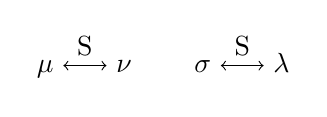
\begin{tikzpicture}

\snode{MU}{0,0}{\mu};
\snode{NU}{1,0}{\nu};
\snode{SIG}{2,0}{\sigma};
\snode{LAM}{3,0}{\lambda};

\draw[<->] (MU) -- (NU) node [midway, above] () {S};
\draw[<->] (SIG) -- (LAM) node [midway, above] () {S};

\end{tikzpicture}
\end{center}
\noindent There are two pairs of connected vertices, which indicates that the integrals can be evaluated with $\ccpx{2}$ effort, which is in agreement with the findings above. The $S$ denotes the overlap relationship between vertices.
For another example, consider the Hartree Fock expression for the exchange matrix
\begin{equation}
K_{\mu\nu} = \cn{\mu\sigma}{\nu\lambda} P_{\lambda\sigma}
\end{equation}
\noindent Diagrammtically, the expression for $\mathbf{K}$ can be represented as
\begin{center}
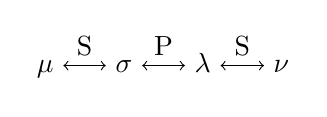
\begin{tikzpicture}

\snode{MU}{0,0}{\mu};
\snode{NU}{3,0}{\nu};
\snode{SIG}{1,0}{\sigma};
\snode{LAM}{2,0}{\lambda};

\draw[<->] (MU) -- (SIG) node [midway, above] () {S};
\draw[<->] (SIG) -- (LAM) node [midway, above] () {P};
\draw[<->] (LAM) -- (NU) node [midway, above] () {S};

\end{tikzpicture}
\end{center}
\noindent The connection between $\sigma$ and $\lambda$ is also known as a "P-junction" (Nee2009), which represents the sparsity relationship arising due to the exponential decay of density matrix elements. The sparsity graph is fully connect, which suggests that $\mathbf{K}$ can be evaluated with $\mathcal{O}(N)$ effort. This is indeed the case, as shown by the ONX or LinK method. For linear scaling to emerge, indices of an expression therefore need to be fully linked. This simple but important fact is also known the linked index rule (LIR). Diagrams also show which factors can influence the performance of the scaling, such as diffuseness of the atomic orbitals (slower S decay) or size of of the HOMO-LUMO gap (slower P decay). One can therefore conclude that the expression for $\mathbf{K}$ as given above, is less suitable for large basis sets and non-insulators.

\subsection{Rank Sparsity}

A positive semi-definite matrix $\mathbf{A}$ has the property that it can be decomposed as a product 
\begin{equation}
\mathbf{A} = \mathbf{B} \mathbf{B}^T
\end{equation}
\noindent where $\mathbf{A}$ has dimensions $N$ by $N$, and $\mathbf{B}$ has dimensions $N$ by $rank(A)$. The rank represents the number of linearly independent column vectors in matrix, and for $rank(A) < N$, the matrix is said to  be rank-deficient. The decomposition matrix $\mathbf{B}$ therefore is more compact and needs less storage space than $\mathbf{A}$. There are different ways to compute $\mathbf{B}$, such as Cholesky decomposition or QR decomposition.
The tensor $\cn{\mu\nu}{\sigma\lambda}$ can be represented as a $N_{AO}^2$
by $N_{AO}^2$0 matrix with combined row indices $I = \mu + N_{AO}*\nu$ and column indices $J = \sigma + N_{AO}*\lambda$. Because the tensor has been shown to be postive semi-definite, there also exists a decomposition, such that
\begin{equation}
\cn{\mu\nu}{\sigma\lambda} = A_{(\mu\nu)(\sigma\lambda)} = B_{(\mu\nu)X} B_{(\sigma\lambda)X}
\end{equation}
\noindent The rank of $\mathbf{A}$ is in general much smaller than the combined index range $N_{AO}^2$, and scales linearly rather than quadratically with the number of basis sets. The decomposition tensor $\mathbf{B}$ is therefore 3-dimensional, rather than 4-dimensional, which reduces the storage needed by an order of magnitude from $\ccpx{4}$ to $\ccpx{3}$, but only in the case where $\cn{\mu\nu}{\sigma\lambda}$ is dense. In the limit of large molecules, the NZEs of $\mathbf{B}$ also scale with $\ccpx{2}$. Rather than for the molecular integrals in the AO basis, decomposition techniques are more useful for reducing the storage size of molecular integrals in the canonical MO basis
\begin{equation}
\cn{ia}{jb} = C_{\mu i} C_{\sigma a} B_{\mu \sigma X} B_{X \nu \lambda} C_{\nu j} C_{\lambda b} = B_{iaX} B_{Xjb}
\end{equation} 
\noindent The AO-MO transformation step is also drastically sped up, but remains a $\ccpx{4}$ effort. Rank sparsity has therefore little impact on the overall scaling, but rather reduces the scaling \emph{prefactor}. Over the years, different methods have been proposed to compute $\mathbf{C}$, such as density fitting, Cholesky decompostion, pseudo-spectral methods, or tensor hypercontraction.
Density matrices at different levels of theory (Hartree Fock, MP2, CC ...) also exhibit rank sparsity. Decomposition of such matrices play an important role in local molecular orbital schemes and low scaling electronic structure methods, as will be shown in later sections.

% pos def Roo1951 C. C. J. Roothaan, Rev. Mod. Phys., 23, 69 (1951).

% Schwarz inequality Has1989 https://onlinelibrary.wiley.com/doi/abs/10.1002/jcc.540100111

% Good explanation for "linked indices rule" https://aip.scitation.org/doi/pdf/10.1063/1.4926879

% Nee2009 https://reader.elsevier.com/reader/sd/pii/S0301010408005089?token=A38BA6311BBE21191E796ADD75EF1602618F281416BBB8E8C22D61B0C75DF4C02EF402A33375738162D7AA02AFAB8685&originRegion=eu-west-1&originCreation=20210707062425

\FloatBarrier

\section{Density Fitting}

The method of choice in this thesis for the decomposition of two-electron molecular integrals is \emph{density fitting} (DF), also knwon as \emph{resoulation of the identity} (RI). For a brief exploration of other popular methods, the reader is referred to (ANNEX).  

\subsection{Basics of Density Fitting}

The two-electron integrals can be expressed in terms of the charge product densities $\rho_{\mu\nu} = \chi_{\mu} \chi_{\nu}$ as
\begin{equation}
\cn{\mu\nu}{\sigma\lambda} = \int \int \frac{\rho_{\mu\nu}(\mathbf{r_1}) \rho_{\sigma\lambda}(\mathbf{r_2}) }{\mathbf{r_1} - \mathbf{r_2}} d\mathbf{r_1} d\mathbf{r_2}
\end{equation}
The charge densities $\rho$ can be approximated by fitting them to a set of atom-centred auxiliary functions $\chi_P$
\begin{equation}
\rho_{\mu\nu}(\mathbf{r}) = C_{P\mu\nu} \chi_{P}(\mathbf{r}) + \Delta \rho_{\mu\nu}
\end{equation}
\noindent Or in the chemist's notation:
\begin{equation}
\cket{\mu\nu} = C_{P\mu\nu} \cket{P} + \cket{\eps_{\mu\nu}} = \cket{\tilde{\mu\nu}} + \cket{\eps_{\mu\nu}}
\end{equation}
\noindent where $C_{P\mu\nu}$ are the fitting coefficients, and $\Delta \rho_{\mu\nu}$ or $\cket{\eps_{\mu\nu}}$ is the error introduced by the fitting procedure. Eq. ... is known as the density fitting approximation (Whi73,Bae1973). The two-electron integrals then take the form
\begin{equation}
\begin{split}
\cn{\mu\nu}{\sigma\lambda} &= (\widetilde{\mu\nu}|\widetilde{\sigma\lambda}) +  \underbrace{(\widetilde{\mu\nu}|\eps_{\sigma\lambda}) + (\eps_{\mu\nu}|\widetilde{\sigma\lambda})}_\textrm{first order} + \underbrace{\cn{\eps_{\mu\nu}}{\eps_{\sigma\lambda}}}_\textrm{second order} \\
&= (\widetilde{\mu\nu}|\widetilde{\sigma\lambda}) + \eps_J^{(1)} + \eps_J^{(2)} 
\end{split}
\end{equation}
\noindent Here, $\eps_J^({1})$ and $\eps_J^({2})$ represent the first order (linear) and second order (quadratic) error. The fitting coefficients are then generally found by minimizing $\eps_J^{(2)}$. Substituting $\cbra{\eps_{\mu\nu}} = \cbra{\mu\nu - \widetilde{\mu\nu}}$ gives
\begin{equation}
\frac{\partial}{\partial C^P_{\mu\nu}} \cn{\mu\nu - \widetilde{\mu\nu}}{\sigma\lambda - \widetilde{\sigma\lambda}} = 0
\end{equation}
\noindent which then yields a set of linear equations
\begin{equation}
\cn{\mu\nu}{P} - \sum_Q C^Q_{\mu\nu} \cn{Q}{P} = 0 
\end{equation}
\noindent Finding the fitting coefficients by minimizing $\eps_J^{(2)}$ has the important feature that $eps_J^{(1)} = 0$, which can be shown by substituting Eq. ... back into Eq. ... . The total electron integral error is therefore \emph{quadratic} in the fitting error. Fitting procedures where the coefficients $C^P_{\mu\nu}$ satisfy Eq. ... are termed $\emph{robust}$ (Dun2000). Any restrictions posed on $C^P_{\mu\nu}$ makes $\eps_{1}$ diffent from zero and the error scales linearly. 
Eq. ... needs the evaluation of the three-centre-two-electron (3c2e) and two-centre-two-electron (2c2e) integrals in the auxiliary basis set $\{P\}$
\begin{equation}
\cn{\mu\nu}{P} = \int \int \chi_{\mu}(\mathbf{r_1}) \chi_{\mu}(\mathbf{r_1}) \frac{1}{\mathbf{r_1} - \mathbf{r_2}} \chi_{P}(\mathbf{r_2}) d\mathbf{r_1} d\mathbf{r_2} 
\end{equation}
\begin{equation}
\cn{P}{Q} = \int \int \chi_{P}(\mathbf{r_1}) \frac{1}{\mathbf{r_1} - \mathbf{r_2}} \chi_{Q}(\mathbf{r_2}) d\mathbf{r_1} d\mathbf{r_2} 
\end{equation}
\noindent The fitting coefficients are generally computed by inverting $\cn{P}{Q}$, which leads to the following approximation for the four-centre-two-electron integrals
\begin{equation}
\cn{\mu\nu}{\sigma\lambda} \approx \cn{\mu\nu}{P} \cn{P}{Q}^{-1} \cn{Q}{\sigma\lambda}
\end{equation}
\noindent Matrix inversion is a $\ccpx{3}$ computational effort. For more details on precision and best practices involving matrix inversion, see ... .
% Introduced independently by
% (Coulomb) Whi73 https://aip.scitation.org/doi/10.1063/1.1679012
% (Overlap) Bae1973 https://doi.org/10.1016/S0301-0104(99)00271-2 2, 41 (1973).
% Dunlap improved Baerends by using coulomb instead of overlap
% Dun1979 https://aip.scitation.org/doi/pdf/10.1063/1.438728
% Dun1979a https://doi.org/10.1063/1.438313 71, 4993 (1979).
% Begriff "Robust" erstmals hier
% Dun2000 https://www.sciencedirect.com/science/article/pii/S0166128099004339?via%3Dihub

\subsection{Scaling of the 3c2e Integrals}

Using the diagrammatic representation introduced earlier, the 3c2e integral tensor reduces to
\begin{center}
\begin{tikzpicture}
\snode{MU}{0,0}{\mu};
\snode{NU}{1,0}{\nu};
\snode{X}{2,0}{P};
\draw[<->] (MU) -- (NU) node [midway, above] () {S};
\end{tikzpicture}
\end{center}
The number of non-zero elements elements therefore scales as $\ccpx{2}$, just like for the 4c2e integrals. Similarly, the Schwarz inequality can be used to screen out small integrals
\begin{equation}
\left\lvert \cn{\mu\nu}{P} \right\rvert \leq \left\lvert \cn{\mu\nu}{\mu\nu} \right\rvert^{1/2} \left\lvert \cn{P}{P} \right\rvert^{1/2}
\end{equation}
\noindent As mentioned above, Schwarz screening does not take into account increasing bra-ket distance. The long-range decay is too slow to be of any advantage in the case of the 4c2e integrals. However, it was found (Hol2015) that for an auxiliary density $\chi_P(\mathbf{r}$ with angular momentum $l_P$, the 3c2e integrals actually decay as $1/R^{-1 - l_P}$ with increasing bra-ket distance, establishing a weak sparsity relationship between $\cbra{\mu\nu}$ and $\cket{P}$ 
\begin{center}
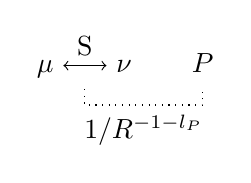
\begin{tikzpicture}
\snode{MU}{0,0}{\mu};
\snode{NU}{1,0}{\nu};
\snode{MUNU}{0.5,0}{};
\snode{X}{2,0}{P};
\draw[<->] (MU) -- (NU) node [midway, above] () {S};
\draw[dotted] (MUNU.south) |- (1.25, -0.5) node [below]{$1/R^{-1-l_P}$} -| (X.south);
\end{tikzpicture}
\end{center}
\noindent In principle, the 3c2e integrals can be evaluated with linear effort. Hollmann et al (Hol2015) have introduced a tight upperbound, known as the SVQl estimator, to exploit this faster decay. Due to the dependence on $l_P$, the screening is most effective with larger basis sets with high angular momentum functions.

The fitting coefficients evaluated as $C^P_{\mu\nu} = \cn{\mu\nu}{Q} \cn{Q}{P}^{-1}$ formerly scale with $\ccpx{3}$
\begin{center}
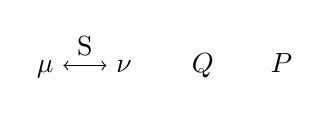
\begin{tikzpicture}
\snode{MU}{0,0}{\mu};
\snode{NU}{1,0}{\nu};
\snode{Q}{2,0}{Q};
\snode{P}{3,0}{P};
\draw[<->] (MU) -- (NU) node [midway, above] () {S};
\end{tikzpicture}
\end{center}
\noindent due to the inverse of $\cn{P}{Q}$ not being sparse. 

\subsection{Local Density Fitting: Principles} 
The long-range behaviour introduced by Eq. ... is often deemed "unphysical" (Tew2019). \emph{Local density fitting} (LDF) methods circumvent this problem by forcing a more rapid decay of long-range contributions, either (a) by using a different metric in the fitting procedure Eq. ... or (b) by constructing domains $[\mu\nu]$ that exclude distant fitting functions $P$ a priori. In both cases, Eq. ... is no longer fulfilled and the error in the electron integrals ... increases linearly with the fitting error, and the density fitting procedure is no longer robust. LDF methods therefore use a different expression for the electron integrals which includes the first order terms to remove the linear error
\begin{equation}
\cn{\mu\nu}{\sigma\lambda} \approx (\widetilde{\mu\nu}|\sigma\lambda) + (\mu\nu|\widetilde{\sigma\lambda}) - (\widetilde{\mu\nu}|\widetilde{\sigma\lambda})
\end{equation}
\noindent which is known as Dunlap's robust density fitting formula. 
 
\subsection{LDF (I): Short-Range Metrics}
The first type of LDF methods replaces the fitting procedure in the Coulomb metric in Eq. ... by a more general expression
\begin{equation}
B_{\mu\nu}^{P} - C_{\mu\nu}^{Q} M_{QP} = 0
\end{equation}  
\noindent where $B_{\mu\nu}^{P}$ and $M_{PQ}$ are the 3-centre- and 2-centre-2-electron integrals given by
\begin{equation}
B_{\mu\nu}^P = \int\int \bfun{\mu}{1}\bfun{\nu}{1} g(\mbf{r_1},\mbf{r_2}) \bfun{P}{2} d\mbf{r_1} d\mbf{r_2}
\end{equation}
\begin{equation}
M_{PQ} = \int\int \bfun{P}{1} g(\mbf{r_1},\mbf{r_2}) \bfun{Q}{2} d\mbf{r_1} d\mbf{r_2}
\end{equation}
\noindent with $g$ being the local metric. A list of known local metrics is given in Table ... . Earliest forms of density fitting actually first used an overlap metric to directly minimizing the norm of the residual $R_{\mu\nu} = \cbra{\mu\nu} - \cbra{\widetilde{\mu\nu}}$ using linear least squares (Baer), and the fitting coefficients are computed as
\begin{equation}
C^P_{\mu\nu} = S_{PQ}^{-1} (\mu\nu Q)
\end{equation}
\noindent where $S_{PQ}$ is the overlap in the auxiliary basis, and $(\mu\nu Q)$ are the 3-centre-\textbf{1-electron} overlap integrals. While the overlap metric has the most rapid decay and the quantities in Eq. can be evaluated in $\mathcal{O}(N)$ time, it has the worst accuracy of all metrics. One solution to this problem is to introduce a metric which is intermediate between overlap and coulomb fitting. Examples include the Yukawa, Coulomb- and Gaussian-attenuated metrics (Table ...). These intermediate metrics introduce a damping factor $\omega$ to control the sparsity and accuracy of the density fit. In the limit where $\omega \rightarrow 0$, and $\omega \rightarrow \infty$, one recovers the coulomb and overlap metric, respectively. Figure ... shows the decay behaviour of a local metric, using the Coulomb-attenuated metric as an example, for $\omega$ = 0.01, 0.1 and 1.0, compared to the overlap and the Coulomb metric. ...

\begin{table}
\makegapedcells
\centering
\begin{tabular}{ccc}
\hline
Type & Ref. & $g(r_{12})$ \\ \hline
Overlap & [A] & 1 \\
Coulomb-Attenuated & [B] & $\dfrac{erfc(\omega r_{12})}{r_{12}}$ \\
Yukawa & [C] & $\dfrac{e^{-\omega r_{12}}}{r_{12}}$ \\
Gaussian-Damped & [D] & $\dfrac{e^{-\omega r_{12}^2}}{r_{12}}$ \\ \hline
\end{tabular}
\caption{Expressions for the operator $g$ in different local metrics.}
\end{table}

\begin{figure}
\centering
\includegraphics[scale=1.0]{ldf.pdf}
\caption{Some caption}
\end{figure}

% A:
% Bae1973 https://www.sciencedirect.com/science/article/pii/030101047380059X?via%3Dihub
% Vah1993 https://www.sciencedirect.com/science/article/pii/0009261493891517?via%3Dihub
% Sky2000 https://www.sciencedirect.com/science/article/pii/S0166128099004340?via%3Dihub
% B: Jun2005 https://www.pnas.org/content/102/19/6692 
% C: Gil2005 https://aip.scitation.org/doi/10.1063/1.2000867 
% D: Rei2008 https://aip.scitation.org/doi/10.1063/1.2956507

% Hol2015 D.S. Hollman, H.F. Schaefer, and E.F. Valeev, J. Chem.Phys.142(2015)

\subsection{LDF (II): Local Domains}

The second method to force locality in density fitting consists in constructing local domains for each atom, pair of atoms or molecular orbital, and excluding any auxiliary functions that lie outside, which can drastically reduce the dimension of the fitting procedure. 

\subsubsection{Atomic Resolution of the Identity}

The simplest example of a domain is one that includes a single atom. The atomic resolution of the identity (ARI) [] uses a fitting procedure where the sum over auxiliary function $Q$ only includes those which are centred on the same atom $A$ as the atomic orbital $\mu$
\begin{equation}
\cket{\widetilde{\mu\nu}} = \sum_{Q \cup A_{\mu}} \cn{P}{Q}_{A_{\mu}}^{-1} \cn{\mu\nu}{Q}
\end{equation}
\noindent Each atom $X$ has its own metric matrix inverse $\cn{P}{Q}_X^{-1}$ which takes the form 
\begin{equation}
\cn{P}{Q}_X^{-1} = B_X \left( \cn{P}{Q}_D + B_X \cn{P}{Q}_{OD}B_X\right)^{-1}B_X
\end{equation}
\noindent where $\cn{P}{Q}_D$ and $\cn{P}{Q}_{OD}$ are the diagonal and off-diagonal part of $\cn{P}{Q}$ respectively. $B_X$ is a so-called \emph{bump matrix} which imposes a fast, but smooth decay between functions $P$ and $Q$ in order to avoid using all functions $P$ for the fitting in Eq. ... . For further details, the reader is referred to the orginal publication. The bump matrix uses multiple distance criteria which make the ARI less of a black-box method.

% Sod2008 https://aip.scitation.org/doi/pdf/10.1063/1.2828533

\subsubsection{Pair-Atomic Resolution of the Identity}

A more popular and simple variant of atomic density fitting is the pair-atomic resolution of the identity (PARI) method (Mer2013). As the name implies, the domains include atom \emph{pairs} rather than a single atom. Again expressing it in terms of the fitting procedure
\begin{equation}
\cn{P}{\mu\nu} = \sum_{Q \in A \cup B} \cn{P}{Q} C^Q_{\mu\nu} \quad \forall P \in A \cup B
\end{equation}
\noindent The number of linear equations is equal to the number of non-zero pairs $\mu\nu$, which scales linearly. However, the PARI approach poses heavy constraints on the fitting coefficients, which leads to large integral errors. Merlot et al. proposed to increase the atomic pair domain with any atoms which lie between A and B. Alternatively, larger and more diffuse basis sets can be used. In both cases, performance is sacrificed for increased accuracy. The abesence of any distance dependent parameters or thresholds still make it an attractive method both for Hartree Fock and Post-Hartree Fock methods (refs).

% Mer2013 https://onlinelibrary.wiley.com/doi/full/10.1002/jcc.23284

\subsubsection{LDF using Local Molecular Orbitals}
Finally, domains can also be formed using local molecular orbitals instead of AOs. LMOs are larger than AOs, but are still generally centred on only a few atoms. The exact atomic sites can be determined for example by using a Mulliken population analysis. Consider the density fitting procedure as proposed by Polly et al. for their LDF-Hartree Fock method (pol2004)
\begin{equation}
\cn{\mu i}{P} = \sum_{Q \in [i]_{fit}} \cn{P}{Q} C^Q_{\mu i}
\end{equation}
The fitting coefficients are determined individually for each AO-LMO pair $\cket{\mu i}$, and include only those auxiliary functions centred on atoms in the fitting domain $[i]_{fit}$ for which the Mulliken charges are above a given threshold. Although the fitting coefficients need to be recomputed for each update of the MO coefficients, the number of $\cket{\mu i}$ pairs scales linearly with system size. This type of local density fitting and variations thereof are predominantly used in pair-orbital specific local correlation methods, and will be explained in more detail further below. 

% Pol2004 Fast Hartree–Fock theory using local densityfitting approximations

\subsection{LDF (III): Quasi-Robust Density Fitting}

Local density fitting inmposes constraints on the fitting procedure, and the integral error consequently scales linearly with the fitting error. Using Dunlap's robust formula is deemed necessary in most cases to achieve acceptable accuracy, but reintroduces the slowly decaying 3c2e integrals. Furthermore, replacing the 4c2e integrals by Eq. ... greatly increases the complexity of expressions in electronic structure theory, which is still manageable for ground state methods, but quickly becomes cumbersome for excited states.

Quasi-robust density fitting (QRDF) aims to combine the exponential decay behaviour of LDF with accuracy comparable to standard density fitting, without the use of Dunlap's formula. Again, consider the fitting procedure 
\begin{equation}
\sum_Q \cn{P}{Q} C^Q_{\mu\nu} = \cn{P}{\mu\nu}
\end{equation}
\noindent The sets of auxiliary functions $\{P\}$ and $\{Q\}$ have different roles. The functions $Q$ fit the charge density $\cket{\mu\nu}$, while the $P$ functions act as \emph{test functions} where the electron integrals should be accurate, i.e. where $\cn{X}{\widetilde{\mu\nu}} \approx \cn{X}{\mu\nu}$. For two functions $\mu$ and $\nu$ not located on the same atom, their charge density $\cket{\mu\nu}$ lies in the vacuum between them, and the atom-centred auxiliary functions may be ill-suited to fit $\cket{\mu\nu}$. For this reason, the fitting procedure draws from all fitting functions $\{P\}$ spanning the whole molecule to cancel out the linear error, which in consequence introduces long-range contributions in $C_{\mu\nu}^P$ in the coulomb metric, even if $\cket{P}$ is not close to $\cket{\mu\nu}$. 
The basic idea of QRDF is to only chose fitting functions $\{P\}$ close to $\cket{\mu\nu}$ via overlap criteria, but still perform the fitting procedure in the coulomb metric.

\subsubsection{The QRDF Fitting Procedure}

For a set of given $\mu,\nu$, select a set of \emph{fitting function} $\{P_{\mu\nu}\} \in \{P\}$ close to $\cket{\mu\nu}$ according to the criteria
\begin{equation}
\left\lvert \sum_R S_{PR}^{-1} (R\mu\nu) \right\rvert > T 
\end{equation} 
\noindent where $S$ is the auxiliary overlap matrix, and $(R\mu\nu)$ are the 1-centre-3-electron overlap integrals. Next, choose a set of test functions $\{Q_{\mu\nu}\} \in \{P\}$ using
\begin{equation}
f(Q_{\mu\nu},P_{\mu\nu}) < R
\label{eq:QRDF_TEST}
\end{equation}
\noindent with
\begin{equation}
f(A,B) = \frac{\alpha \beta}{\alpha + \beta} \left\lvert \mathbf{A} - \mathbf{B} \right\rvert^2
\end{equation}
\noindent where for two auxiliary functions $A$ and $B$, the values $\alpha$, $\beta$ are their smallest primitive exponents and $\mathbf{A}$, $\mathbf{B}$ are their respective positions. The fitting coefficients are then determined via
\begin{equation}
\sum_P \cn{Q_{\mu\nu}}{P_{\mu\nu}} C^P_{\mu\nu} = \cn{Q_{\mu\nu}}{\mu\nu}
\end{equation}
\noindent where the fitting coefficients are accurate within the set of test functions $\{Q_{\mu\nu}\}$. The linear equations in Eq. ... can be solved via QR decomposition of the rectangular matrix $\cn{Q_{\mu\nu}}{P_{\mu\nu}}$.
The QRDF scheme depends on two parameters, $T$ and $R$. In the limit where $T \rightarrow 0$ and $R \rightarrow \infty$, the standard fitting procedure in the coulomb metric is recovered. 

The fitting functions $\{P_{\mu\nu}\}$ are selected via overlap criteria and therefore scale linearly with the number of pairs $\cket{\mu\nu}$, and consequently the same holds true for the number of test functions $\{Q_{\mu\nu}\}$ close to $\{P_{\mu\nu}\}$ chosen by Eq. ... . In the limit of large molecules, the size of the rectangular matrix in Eq. ... becomes constant and the fitting procedure can be evaluated with $\mathcal{O}(N)$ effort. However, a QR decomposition needs to be computed for each set of $\cket{\mu\nu}$, leading to relatively high prefactor which makes the method unuseable for dense 3D structures like water clusters, as will be discussed in the results section.
The QRDF method has been shown to deliver accuracies comparable to standard density fitting, without the use of Dunlap's formula, making it a very attractive alternative to other LDF schemes, especially if one wishes to reduce the complexity of expressions involving LDF.

\subsection{Auxiliary Basis Sets}

The density fitting approximation does not make any assumptions about the size or shape of the auxiliary basis set used. In principle, the fit is exact for the basis set containing all $N_{AO}^2$ gaussian products $\chi_P = \chi_{\mu} \chi_{\nu}$. In practice, the product space is over-complete and can be represented by much smaller basis sets. Accurate results can be obtained for auxiliary basis sets which are about 4 times larger than the principal basis set they are used with. 

Auxiliary basis sets generally need more higher angular momentum functions than standard basis sets. Consider an isolated, unperturbed atom, with electrons occupying atomic orbitals with highest angular momentum $l_{occ}$. A minimal basis set for this atom contains functions of angular momenta 0 to $l_{occ}$. However, a minimal auxiliary basis set for fitting the product space $\chi_{\mu}^{0...l_{occ}} \chi_{\nu}^{0...\l_{occ}}$ needs functions with maximum angular momentum $2l_{occ}$. For example, 2nd row elements ($l_{occ}$ = 1) need an auxiliary basis set containing d-functions, and first row transition metals ($l_{occ}$ = 2) even need g-functions. Similarly to standard basis sets, to describe atoms in molecules where the orbitals are subject to polarization effects, even higher angular momentum functions are needed to fit polarization functions. In practice, a principal basis set with maximum angular momentum $l_{bas}$ is paired with an auxiliary basis set with highest angular momentum $l_{bas} + l_{occ}$. 

Auxiliary basis sets have the drawback of being method-specific. There are two categories: auxiliary basis sets for density fitted Hartree Fock (DF-HF) and for density fitted correlated methods (e.g. DF-MP2, DF-CCSD, DF-ADC(2)). Auxiliary basis sets for DF-HF not only need to reproduce Hartree Fock energies, but also need to minimize theor impact on post-Hartree methods. An ill-suited auxiliary basis set leads to a deterioration of the virtual orbital space, and hence an increased error for correlated methods. 

Optimization procedures often try to minimize the energy differences between the standard method and its density fitting approximation in a series of atomic calculations. For example, the jkfit family of basis sets (cc-pVXZ-JKFIT [Wei2002], def-XVP-JKFIT [Wei2007]) minimize the error
\begin{equation}
\Delta E_{HF} = E_{HF} - E_{DF-HF}
\end{equation}
The RI basis set family (cc-pVXZ-RIFIT (Wei1998), def2-XVP-RIFIT (Ber1998)) minimize the same energy difference but for MP2 or Coupled Cluster. 

Another disadvantage of auxiliary basis sets is that the accuracy of the fitting procedure cannot be easily controlled as a function of its composition (number of functions, angular momenta...), but rather extensive benchmarks are needed for each basis set that is introduced. An alternative approach was proposed by Aquilante et al. (Aqu2007) where the fitting basis sets are generated automatically by cholesky decomposition of the atomic 2-electron integrals
\begin{equation}
\cn{\mu\nu}{\sigma\lambda} = L^X_{\mu\nu} L^X_{\sigma\lambda}
\end{equation}
\noindent The choleksy vectors $\mathbf{L}_{\mu\nu}$ indicate which product densities should be taken to construct the auxiliary basis. This type of atomic Cholesky decompositon (aCD) basis sets has the adavantage that the accuracy can be rigorously controlled by the decompostion threshold $\theta$. To remove linear dependicies in the aCD basis set, another Cholesky decomposition can be performed to yield the atomic compact Cholesky decomposition (acCD) auxiliary basis set (Aqu2009).

% Dunning JKFIT (1): Wei2002 https://pubs.rsc.org/en/content/articlepdf/2002/cp/b204199p
% Karlsruhe JKFIT (2): Wei2007 https://onlinelibrary.wiley.com/doi/full/10.1002/jcc.20702
% MP2 Karlsruhe Wei1998 https://www.sciencedirect.com/science/article/pii/S0009261498008628
% Dunning (MP2) Ber1998 https://aip.scitation.org/doi/pdf/10.1063/1.476732
% Aqu2007 https://aip.scitation.org/doi/10.1063/1.2777146
% Aqu2009 https://aip.scitation.org/doi/10.1063/1.3116784

\section{Multipole Expansion of the Electron Integrals}

The slow $1/R$ between the product densities $\Omega_{\mu\nu}$ and $\Omega_{\lambda\sigma}$ in the coulomb integrals is a major obstacle for achieving linear scaling in cases where no other sparsity relationship can be stablished between indices beclonging to separate charge densities, e.g. in the evaluation of the coulomb matrix $\mathbf{J}$ versus the exchange matrix $\mathbf{K}$. Luckily, there are approximate methods for integral evaluation that can be computed with $\mathcal{O}(N)$ effort, known as \emph{multipole methods}.

\subsection{Classical and Non-Classical Electron Integrals}

First, one needs to introduce the concept of classical and non-classical interactions. Two electron integrals are said to be \emph{non-classical} if the two charge densities $\Omega_{\mu\nu}$ and $\Omega_{\sigma\lambda}$ overlap, and \emph{classical} if the charge densties are well separated. In the latter case, the electron integrals represent classical interactions between disjoint point charges [ref], and can be approximated using multipole methods, whereas the non-classical contributions must be evaluated using the more expensive standard integral codes such as McMurchie-Davidson or Obara-Saika. 

Two gaussian distributions $\Omega_P$ and $\Omega_Q$ are considered \emph{well-separated} up to a target accuracy 10$^{-k}$, if their centre-to-centre distance $R_{PQ}$ is larger than the sum of their extents $ext_P$ and $ext_Q$:
\begin{equation}
R_{PQ} > ext_P + ext_Q
\end{equation} 
\noindent with the extent of a gaussian product $P$ defined as 
\begin{equation}
r_P = \frac{1}{\sqrt{p}} erfc^{-1}(10^{-k})
\end{equation}
\noindent where $p$ is the reduced exponent as given in Equation 0. Another important thing to note is that the number of significant non-classical and classical integrals scale as $\mathcal{O}(N)$ and $\ccpx{2}$ respectively (ref), which has important consequences as will be shown further below. 

\subsection{Multipole Expansion}

For two well-separated charge distributions $P$ and $Q$, the inverse interelectronic distance can be exapanded in terms of Legendre polynomials $\mathcal{P}$ as
\begin{equation}
\frac{1}{r_{12}} = \sum_{l=0}^{\infty} \frac{\Delta r_{12}^l}{R_{PQ}^l} \mathcal{P}_{l} cos \theta
\end{equation}
\noindent with 
\begin{equation}
cos \theta = \frac{\Delta \mathbf{r}_{12}^l \mathcal{R}_{QP}}{\Delta r_{12} R_{QP}} 
\end{equation}
\begin{equation}
\Delta \mathbf{r}_{12} = \mathbf{r}_{1P} \mathbf{r}_{2Q}
\end{equation}
\noindent where $\mathbf{r}_{1P}$ and $\mathbf{r}_{2Q}$ are the distance between electron 1,2 and the centres $P$,$Q$. Equation ... is also known as the partial-wave expansion of the coulomb operator (Arfk1970). Plugging Equation ... into Equation gives the bipolar multipole expansion of the two-electron integrals
\begin{equation}
g_{abcd} = \sum_{l=0}^{\infty} \sum_{m=-l}^l \sum_{j=0}^{\infty} \sum_{k=-j}^{j} M_{ab}^{lm}(P) T_{lm,jk} M_{cd}^{jk}
\end{equation}
\noindent where $\mathbf{M}_{ab}^{lm}(P)$ is the multipole moment of the charge distribution $P$ with total moment $l+k$, and $\mathbf{T}$ is the so-called interaction matrix. As such, the complicated 6-dimensional evaluation of $g$ can be simply substituted by two 3-dimensional integrations of the multipole moments $\mathbf{M}$ at a much lower cost. For the lowest order expansion, where $l$ = $m$ = 0, and $j$ = $k$ = 0, the multipole moments and the interaction matrix become 
\begin{equation}
M_{ab}^{00} = S_{ab}
\end{equation}
\begin{equation}
M_{cd}^{00} = S_{cd}
\end{equation}
\begin{equation}
T_{00,00} = 1/R_{PQ}
\end{equation}
\noindent The zero order term of the multipole expansion therefore takes the form
\begin{equation}
g_{abcd} \approx \frac{S_{ab}S_{cd}}{R_{PQ}}
\end{equation}

\subsection{Fast Multipole Method}

While the number of individual non-zero integrals still scales with $\ccpx{2}$, the total contribution of all pair-wise interactions to the total energy (Hartree Fock, MP2 ...), can actually be evaluated in $\mathcal{O}(N)$.

For the sake of simplicity, consider system with point-charge particles with charge $Z$, in a 2-dimensional plane. The total interaction energy is given by
\begin{equation}
U = \sum_{i>j} \frac{Z_i Z_j}{r_{ij}}
\end{equation}
\noindent Evaluating Equation ... as is takes a quadratic effort. In a first approximation, one can divide the plane into a grid of blocks of equal size, where each block contains a certain number of particles (Figure ...). Consider the interaction of a single particle $i$ in its source block $C$ with the other particles in the system. The interaction has two contributions: near-field (NF) contributions $U_{NF}$ from the other particles in the source block, and the blocks immediately surrounding it, and far-field (FF) contributions $U_{FF}$ from boxes that are well-separated from $C$. The NF interactions are evaluated directly by summing over all particles $j$ in the near-field
\begin{equation}
U^{NF}_i = \sum_{j \in NF} \frac{Z_i Z_j}{R_{ij}}
\end{equation}
\noindent while FF interactions are computed using multipole expansions $\mathbf{q}_{iC}$ and $\mathbf{q}_A$ of the FF boxes and the particle $i$
\begin{equation}
U^{FF}_i = \sum_{A \in FF} \mathbf{q}_{iC} \mathbf{T}_{CA} \mathbf{q}_A
\end{equation}
\noindent While evaluating the interaction energy at block-level rather than particle-level can considerably reduce the prefactor, the cost of this \emph{single-level multipole level} is still quadratic, since for each particle $i$, there is a system-dependent number of FF boxes. The granularity of the blocks is the same, independent of how far away the blocks are. To achieve linear scaling, the crucial point to realize is that, the further one gets from the source block $C$, the smaller the single-particle interaction $U_i$ becomes, and the less accurately it actually needs to be evaluated. This means that the farther one moves away from C, the larger the FF boxes can be. For this reason, \emph{multi-level multipole methods} introduce a hierarchy of boxes (Figure ...), where at level 0, the whole system is in a single box, and for each subsequent level, the field is divided into fourths. FF boxes that are closest to C are evaluated at the highest level/granularity $S$. The region of FF boxes sourrounding the closest FF boxes are then treated at a lower level $S-1$, and so on, until all interactions have been computed. Because the multipole expansion is evaluated for increasing box size, it can be shown that the total number of boxes is constant for a single particle $i$. This is the basic idea on which the \emph{Fast Multipole Method} (FMM) operates [refs], and it has quickly become one of the most important algorithms in scientific computing, as the problem of particle-particle interaction is not limited to the field of quantum chemistry. FMM can evaluate the total interaction energy $U$ with linear computational complexity.

\begin{figure}
\centering
\includegraphics[scale=0.35]{Pics/FMM1}
\caption{A nice caption}
\end{figure}

\begin{figure}
\centering
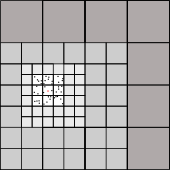
\includegraphics[scale=0.5]{Pics/FMM2}
\caption{Another caption}
\end{figure}

% Gre1987 L. Greengard and V. I. Rokhlin, J. Comput. Phys. 73, 325 (1987)
% Gre1994 L. Greengard, Science 265, 909, (1994)
% Din1992 H. Q. Ding, etc.... look at 28, 29 p. 426 big book

\subsection{Continuous Fast Multipole Method}

The fast multipole method does not work for continuous charge distrbutions like Gaussian functions, as their extents can be quite different from one another, making the separation into NF and FF contributions more difficult. Nonetheless, FMM has been generalized to the continous case, known as the continuous fast multipole method (CFMM) (ref). The principle is the same as in multi-level multipole methods, only special care needs to be taken to only include classical contributions into the FMM treatment. For further details, the reader is referred to the original publication. 

% Ark1970 https://www.sciencedirect.com/book/9780123846549/mathematical-methods-for-physicists


\section{The ABCs of LMOs: Orbital Representations \label{sec:ABCLMO}}

A small intro

%\url{https://link.springer.com/article/10.1007/s00894-018-3880-8}

Occupied and virtual molcular orbitals can generally be represented in two ways: canonical molecular orbitals (CMOs) and local molecular orbitals (LMOs). CMOs are the eigenvectors of the Fock matrix obtained by solving the eigenvalue problem

\begin{equation}
\mathbf{F}\mathbf{C} = \mathbf{S}\mathbf{C} \eps
\end{equation}

where the eigevalues $\epsilon$ are known as the molecular orbital energies of the associated CMOs. However, CMOs are not unique in the sense that there are multiple molecular representations possible which yield the same electron density $\mathbf{P}$. Observables such as the electron density, or the total energy, are said to be invariant under unitary transformations (Fock V (1930) Z Phys 61:26–148). The CMOs $\mathbf{C}$ relate to other representations $\mathbf{L}$ as

\begin{equation}
L_{\mu \uli} = U_{\uli i} C_{\mu i}
\end{equation}

\noindent where $\mathbf{U}$ is a unitary transformation matrix with $\mathbf{U}^{\dagger} \mathbf{U}$ = $\mathbb{1}$. Typically, $\mathbf{U}$ is chosen to generate a set of molecular orbitals which are localized on as few atoms as possible, hence local molecular orbitals. While CMOs and LMOs agree on observables, they show differences for non-obervables, such as molecular orbital energy or orbital shape.

There are several reasons for choosing an LMO representation. First, as mentioned above, LMOs are used in local correlation methods, because CMOs are too delocalized, and electron correlation between LMO centres decay more rapidly. Secondly, they offer a more intuitive picture for chemists and help to interpret chemical phenomena (cite), e.g. invloving lone pairs or $\pi$ bonds. Different representations can be used to interpret different phenomena, e.g. Boys LMOs vs NTOs.

Over the years, a myriad of different schemes has been proposed on how to find appropriate tranformation matrices $\mathbf{U}$. We will now go over some examples.

\subsection{Local Molecular Orbitals}

Some words about it

\subsection{LMOs by Reducing a Functional}
% (0) https://aip.scitation.org/doi/full/10.1063/1.2360264
% (1) https://journals.aps.org/rmp/abstract/10.1103/RevModPhys.32.296
% (2) https://journals.aps.org/rmp/abstract/10.1103/RevModPhys.35.457
% (3) https://aip.scitation.org/doi/10.1063/1.456588
% (4) J. E. Subotnik, Y. Shao, W. Z. Liang, and M. Head-Gordon, J. Chem. Phys. https://doi.org/10.1063/1.1790971 121, 9220 (2004).
% (5) https://aip.scitation.org/doi/10.1063/1.2033687

One of the most popular methods for finding LMOs consists in maximizing a localization function $\eta(\phi)$ by successive rotation of the orbital space. The most prominent examples are Foster-Boys (FB)(1), Edmiston-Ruedenberg (ER) (2) and Pipek-Mezey (PM) (3). Their functionals can be written as

\begin{eqnarray}
\zeta_{FB}(\chi) = \sum_i \bra{\chi_i} \mathbf{r} \ket{\chi i}^2 \\
\zeta_{ER}(\chi) = \sum_i \cn{\chi_i \chi_i}{\chi_i \chi_i} \\
\zeta_{FB}(\chi) = \sum_i \sum_A \bra{\chi_i} \mathbf{P}_A \ket{\chi i}^2 
\end{eqnarray}

The problem is generally solved using an iterative procedure consisting in consecutive pair-wise rotations, known as Jacobi sweeps (ALGO). These sweeps are rotated until convergence is reached, which may be slow. The methods differ within the procedure by how the rotational angle is computed, and scale diiferently with system size, with $\ccpx{3}$ for FB, $\ccpx{5}$ for ER and $\ccpx{4}$ for PM. A faster alternative to Jacobi sweeps does also exist (4). 

Over the years, PM has been the more popular choice of the three: like ER and unlike FB, it conserves $\sigma$-$\pi$ separation (0),  but it scales more favorably than ER.

Functional localization methods are most often used for rotating occupied MOs. Virtual MOs are often plagued by convergence issues and have a steep computational cost simply due to being much more numerous than occupied MOs (5). It is crucial that molecular localization should not take longer than the methods they are used for, and hence VMOs are often localized using separate methods.

EXAMPLES!! Ethylene

\subsection{Projected Atomic Orbitals}
% (0) https://www.annualreviews.org/doi/10.1146/annurev.pc.44.100193.001241
% (1) https://aip.scitation.org/doi/full/10.1063/1.2173249

A set of highly localized molecular orbitals can be obtained by projecting the CMOs onto the atomic orbital basis, known as projected atomic orbitals (PAO) (0). For a set of orthonormal occupied and virtual molecular orbitals $\{\Psi_i\}$ and $\{\Psi_a\}$, the projection operators $\hat{P}$ and $\hat{Q}$ are defined as (1)

\begin{eqnarray}
\hat{P} &= \ket{\Psi_i} \bra{\Psi_i} &= \ket{\chi_{\mu}} C_{\mu i} C_{\nu i} \bra{\chi_{\nu}} \\
\hat{Q} &= \ket{\Psi_a} \bra{\Psi_a} &= \ket{\chi_{\mu}} C_{\mu a} C_{\nu a} \bra{\chi_{\nu}}
\end{eqnarray}

\noindent which are then applied to the atomic orbitals $\chi$ 

\begin{eqnarray}
\hat{P} \ket{\chi_{\mu'}} &= \sum_{\mu} P_{\mu\nu} S_{\nu\mu'} \ket{\chi_{\mu'}} &= \sum_{\mu} \ovl{P}_{\mu \mu'} \ket{\chi_{\mu'}} = \ket{\chi_{\ulgm}} \\
\hat{Q} \ket{\chi_{\mu'}} &= \sum_{\mu} Q_{\mu\nu} S_{\nu\mu'} \ket{\chi_{\mu'}}  &= \ovl{Q}_{\mu \mu'} \ket{\chi_{\mu'}} = \ket{\chi_{\olgm}}
\end{eqnarray} 

The projection operators $\hat{P}$, $\hat{Q}$ and the non-symmetric PAO coefficient matrices $\mathbf{\ovl{P}}$, $\mathbf{\ovl{Q}}$ are \emph{idempotent}
\begin{equation}
\mbf{\ovl{P}}\mbf{\ovl{P}} = \mbf{\ovl{P}} \qquad
\mbf{\ovl{Q}}\mbf{\ovl{Q}} = \mbf{\ovl{Q}}
\end{equation}

\noindent and \emph{mutually orthogonal} 
\begin{equation}
\mbf{\ovl{P}}\mbf{\ovl{Q}} = \mbf{0} \qquad \mbf{\ovl{P}} + \mbf{\ovl{Q}} = \mbf{1} 
\end{equation} 

\noindent But not orthogonal within themselves
\begin{equation}
\bra{\chi_{\ulgm}} \ket{\chi_{\ulgn}} = S^{PAO}_{\ulgm\ulgn} \qquad \bra{\chi_{\olgm}} \ket{\chi_{\olgn}} = S^{PAO}_{\olgm\olgn}
\end{equation}
The number of PAOs (occupied or virtual) is equal to the number of AOs, and are therefore linearly dependent (redundant). CMOs are transformed to PAOs by using
\begin{eqnarray}
\ket{\chi_{\ulgm}} &= (\mathbf{SC})_{\mu i}  \ket{\Psi_i} &= \ovl{C}_{\mu i} \ket{Psi_i} \\
\ket{\chi_{\olgm}} &= (\mathbf{SC})_{\mu a} \ket{\Psi_a} &=  \ovl{C}_{\mu a} \ket{\Psi_a}
\label{CMO2PAO}
\end{eqnarray}
\noindent The back-transformation is defined as
\begin{eqnarray}
\ket{\Psi_{i}} &= C_{\mu i} \ket{\ulgm} \\
\ket{\Psi_{a}} &= C_{\mu a} \ket{\olgn} 
\label{PAO2CMO}
\end{eqnarray}
PAOs are centred on the atom on which their corresponding AO is localized, but can still be delocalized over multiple atoms, depending on the sparsity of the density matrix. Methods which are entirely formulated in PAOs are rare but possible (1). The projection method is most often used on the virtual orbital space, where standrad localiztaion procedures fail. A set of virtual PAOs is generated from LMOs by using the orthogonality relationship from Eqaution ...
\begin{equation}
\mbf{\ovl{Q}} = \left( \mbf{1} - \mbf{LL}^{\dagger} \mbf{S} \right) \mbf{C} 
\end{equation}

\subsection{Subspace Projected Atomic Orbitals}

Some applications need localized molecular orbitals that only span a certain region of a molecule, e.g. density matrix embedding theory (DMET) (refs) or local ADC (ref). The molecule is split into two subunits, and atoms are grouped into an active region $A$ and an inactive region $B$ according to specific selection criteria. Region $A$ contains the molecular subunit of interest. 

Most implementations use the Mulliken gross charges to find
... ? Not used for virtuals? Put it into AO-ADC Part?

% SPADES: Cla https://www.osti.gov/pages/servlets/purl/1631165
% SPADES: Cla2019 https://pubs.acs.org/doi/10.1021/acs.jctc.8b01112

\subsection{Cholesky Molecular Orbitals}

Sparsity of the atomic density matrix is crucial for achieving low-scaling electronic structure methods. Aquilante et al. proposed (0) to define a set of occupied molecular orbitals by Cholesky decomposition of the density matrix. Analysis of the resulting Cholesky molecular orbitals (CholMOs) showed their localized character inherited from the sparsity of the density matrix.

\begin{equation}
\mathbf{P} = \mathbf{LL^T}
\end{equation}

Figure ... shows the sparsity of the occupied density matrix and the occupied cholesky molecular coefficient matrix of the linear alkane H$_{322}$C$_{160}$. The number of CholMOs is equal to the rank of the density matrix, which is equal to the number of occupied orbitals. The CholMOs are computed by an incomplete Cholesky decomposition with full row and column pivoting  (ALGO). The unitary transformation matrix is given by

\begin{equation}
U_{i\uli} = C_{\mu i} S_{\mu \nu} L_{\nu \uli}
\end{equation}

The decomposition algorithm scales with $\ccpx{3}$ but can be made linearly scaling by using sparse matrix algebra. CholMOs have several advantages: the Cholesky decomposition is fast and non-iterative, and an initial guess for molecular orbitals is not needed. 

The scheme can be extended to virtual orbitals as well, by CD of the virtual atomic density matrix $\mathbf{Q}$. The rank of $\mathbf{Q}$ is equal to the number of virtual orbitals $n_vir$, therefore the prefactor of the incomplete CD increases with basis set size. Especially in the presence of diffuse functions, the rank reduction might not offer much of an advantage compared to simpler localization methods such as PAOs.  

Moreover, orbitals obtained by CD are less localized than FB or ER LMOs, especially for small molecules. Low scaling is still possible using CholMOs in the context of LMO correlation methods, albeit with a larger prefactor.

CD is also used in the context of AO-MP2 to reduce the prefactor of inetgral transformation by using the rank sparsity of the pseudo-density matrices, as will be shown further below.

CholMOs can also used as an initial guess for iterative localization schemes to achive faster convergence.

\begin{figure}[h]
\centering
\begin{subfigure}{0.5\linewidth}
\centering
\includegraphics[scale=1.0]{densityO}
\end{subfigure}
$\Longrightarrow$
\begin{subfigure}{0.4\linewidth}
\centering
\includegraphics[scale=1.0]{choleskyO}
\end{subfigure}%
\hfill
\centering
\begin{subfigure}{0.5\linewidth}
\centering
\includegraphics[scale=1.0]{densityV}
\end{subfigure}
$\Longrightarrow$
\begin{subfigure}{0.4\linewidth}
\centering
\includegraphics[scale=1.0]{choleskyV}
\end{subfigure}%
\caption{Something}
\end{figure} 

\subsection{Natural Orbitals}

While the schemes described above try to generate a set of occupied and/or virtual molecular orbitals localized in space, natural orbital (NOs) methods try to generate a set of "compact" orbitals, i.e. a minimal set of orbitals that can describe the problem at hand. The concept of natural orbitals was first introduced by Löwdin (A). The natural orbitals $\Theta_i$ of a wave function $\Psi$ are defined as the eigenfunctions of the one-particle density operator $\hat{n}$

\begin{equation}
\hat{n}\ket{\Theta_i} = n_i \ket{\Theta_i} 
\end{equation}

\noindent where $n_i$ are the occupation numbers of the associated orbital $\Theta_i$. One can then choose a reduced orbital space $\{\tilde{\Psi}_i\}$ by only taking into account those orbitals with an occupation number above a certain threshold $\tau$. The orbitals are "natural" in the sense that they are determined purely using $\Psi$, and are intrinsic to the system. NOs are computed by diagonalizing the one-particle density matrix at the desired level of theory (Hartree-Fock, MP, CIS, CC). 

NOs are state-specific (Pok2019), meaning that NOs computed from the ground state densities may not be well suited to describe excited states, and NOs of different excited states might also greatly differ. As such, as will be later shown for local flavours of ADC, NOs need to be recomputed for each state.

% CIS(D) density matrices https://aip.scitation.org/doi/pdf/10.1063/1.4983277

\subsubsection*{Natural Orbitals in Hartree Fock Theory}

In Hartree Fock theory, natural orbitals are mostly reserved for qualitative population and bond order analysis. 

Natural atomic orbitals (NAOs) are computed by diagonalizing the blocks $P_{\mu_A\nu_A}$ of the atomic density matrix, where ${\mu_A}$, ${\nu_A}$ are basis functions centred on atom $A$. NAOs are optimal for describing the electron density around individual atom centres (IUPAC). NAOs are also useful for obtaining a set of guess orbitals from densitiy matrices formed from the superposition of atomic densities (SAD) guess. 

NHOs obtained from NAOs + off-diag NAOs 
% (ref: https://pubs.acs.org/doi/pdf/10.1021/ja00544a007)

NBOs obtained from NHOs

% NBOs https://aip.scitation.org/doi/pdf/10.1063/1.445134

% NAOs, NBOs https://pubs.rsc.org/en/content/articlepdf/2001/rp/b1rp90011k

% (Recent) NBOs https://onlinelibrary.wiley.com/doi/epdf/10.1002/wcms.51

% https://goldbook.iupac.org/terms/view/NT07076

\subsubsection*{Frozen Natural Orbitals}

For large basis sets, CMOs are much more compact than the virtual orbital span, and the number of occupied NOs is not significantly lower than that of occupied CMOs. It is therefore sufficient to only compute the eigenfunctions of the virtual-virtual block of the one-particle density matrix, which are known as frozen natural orbitals (FNOs) (Bar1970). FNOs need information of the correlated wave function, and are therefore typically computed at a lower level of theory. For example, the easiest way to obtain a set of FNOs for CCSD or CCSD(T) computation is to diagonalize the virtual-virtual block  of the MP2 density matrix (Sos1989, Tau2005, Tau2008)
\begin{equation}
D_{ab} = \frac{1}{2} sum_{cij} \frac{K_{ij}^{cb} K_{ij}^{ca}}{\eps_{ij}^{ab} \eps_{ij}^{ca}}
\end{equation}
\noindent with
\begin{equation}
K_{ij}^{ab} = 2 \cn{ia}{jb} - \cn{ib}{ja}
\end{equation}
\begin{equation}
\eps_{ij}^{ab} = \eps_i + \eps_j - \eps_a - \eps_b 
\end{equation}
The FNOs are then canonicalized (see ...). The combined set of occupied CMOs and virtual FNOs forms a very compact representation suitable for CC ground state and excited state calculations.

% MP2 NOs:
% Jor1988 J. Chem. Phys. 88, 3834 (1988); https://doi.org/10.1063/1.453884
% D. M. Silver and R. J. Bartlett,Phys. Rev. A13,1 1976.
% D. M. Silver, S. Wilson, and R. J. Bartlett,Phys. Rev. A16,477 1977.

% FNOs: 
% Bar1970 Phys. Rev. A 1, 644 – Published 1 March 1970

% FNO CC: 
% Sos1989 https://doi.org/10.1016/0009-2614(89)87399-3
% Tau2005 Taube, Andrew G.; Bartlett, Rodney J. (2005). Frozen Natural Orbitals: Systematic Basis Set Truncation for Coupled-Cluster Theory. Collection of Czechoslovak Chemical Communications, 70(6), 837–850. doi:10.1135/cccc20050837  
% A. G. Taube and R. J. Bartlett,  Frozen natural orbital coupled-cluster theory:  Forces andapplication to decomposition of nitroethane,  J. Chem. Phys.128, 164101 (2008)
% CCLR NO  A. Kumar and T. D. Crawford,   Frozen virtual natural orbitals for coupled-cluster linear-response theory,  J. Phys. Chem. A121, 708 (2017).

% Have a look at Pok2019 https://chemrxiv.org/articles/preprint/Extension_of_Frozen_Natural_Orbital_Approximation_to_Open-Shell_References_Theory_Implementation_and_Application_to_Single-Molecule_Magnets/10308053/1

\subsubsection*{Natural Transition Orbitals}

Consider the CIS eigenvalue problem for finding the excitation energies $\omega_n$ and their associated transition density matrices $R_n$

\begin{equation}
\mathbf{A_{CIS}} R_n = \omega_n R_n 
\end{equation}

The matrices $\mathbf{R}_n$ contain $n_{occ}n_{vir}$ expansion coefficients $c_{ia}$ which show how much an orbital-virtual MO pair $ia$ contributes to the excitation $n$. The numer of non-negligebale coefficients can be far from zero, making interpretations of the computed results difficult for some systems.

Natural transition orbitals (NTOs) were introduced to facilitate the qualititative description of an excited state and finding connections to experimental spectra (Luz1976, Mar2003, Mar2008). NTOs are typically obtained by computing the singular value decomposition (SVD) of the state densities $\mathbf{R}_n$

\begin{equation}
\mathbf{R} = \mathbf{U} \mathbf{\Sigma} \mathbf{V}^{\dagger}  
\end{equation} 

\noindent where $\mathbf{U}$ and $\mathbf{V}$ are unitary matrices with dimension $n_{occ} n_{NTO}$ and $n_{vir}n_{NTO}$, and $\Sigma$ is a $n_{NTO}$ by $n_{NTO}$ matrix containg the singular values $s$ on its diagonal. The CMOs $\{\Psi^{occ}_i,\Psi^{vir}_a\}$ are transformed to the NTO basis $\{\overline{\Psi}^{occ}_k,\overline{\Psi}^{vir}_k\}$ using

\begin{equation}
\ket{\overline{\Psi}^{occ}_k} = U_{ki} \ket{\Psi^{occ}_i}
\end{equation}
\begin{equation}
\ket{\overline{\Psi}^{vir}_k} = V_{ka} \ket{\Psi^{vir}_a}
\end{equation}

\noindent The singular value $s_k$ show the contribution of an NTO pair $k$ to the excited state. In most cases, the number of significant NTO pairs is significantly lower than $n_{occ}n_{vir}$ and at most equal to $n_{occ}$. NTOs are not limited to CIS, but can also be obtained by SVD decomposition of the singles-singles block of excited state densities from higher order methods such as ADC or CCLR. 

Natural transition orbitals have also found use in local excited  state correlation methods (Bau2017,Hof2017), where CIS NTOs are combined with MP2 NOs to obtain a compact orbital representation for ground and excited state coupled cluster calculations.

EXAMPLE!!! phenylalanine

% Luz1976 https://link.springer.com/article/10.1007%2FBF00526670

% Mar2003 https://aip.scitation.org/doi/pdf/10.1063/1.1558471

% https://www.sciencedirect.com/science/article/pii/S0009261407002072?via%3Dihub

% CornFlex: Bau2017 https://aip.scitation.org/doi/pdf/10.1063/1.4984820

% Hof2017 Natural transition orbitals for the calculation of correlation andexcitation energies


\subsection{Specific Virtual Orbitals}

In most cases, using LMOs instead of CMOs does not offer any a priori advantage in terms of the computational complexity asscociated with correlated methods, and additional approximations are necessary. In local correlation methods, this is often done by truncating the VMO space. TRuncation of the VMOs has been an active field of research for "a long time", and several schemes have emerged over the years. A naive approach to truncate the virtual space would be to eliminate VMOs with orbital energies above a certain threshold; however, this proved to be unusable in most contexts (ref). More successful methods for VMO truncation use the concept of what we will refer to as \emph{specific virtual orbitals} (SVOs). SVOs are specific in the sense that each individual occupied LMO $i$ or each pair of LMOs $ij$ has their own set of SVOs $a_i$ (orbital specific virtual orbitals) or a$_{ij}$ (pair specific virtual orbitals) associated to it.
The concept of SVOs naturally arises in the context of correlated methods such as the coupled electron pair approximation (CEPA) where the total energy is computed is computed as the sum of electron pair energies $e$
\begin{equation}
E_{CEPA} = \sum_{ij} e_{ij}
\end{equation}
The electron pair energy decays rapidly as a function of the distance $r$ between MO centres in an LMO basis. Distant virtual orbitals contribute less to the elctron pair energy as virtual orbitals close to ${ij}$. It has been shown early on that instead of using the whole virtual orbital span, one can correlate only a subset or reduced set of virtual orbitals with each electron pair (0,1,2,3) and still recover most of the correlation energy. In the limit of large molecules, the number of signiciant virtual orbitals for an electron pair becomes independent of system size (4). There are different ways to choose how to define the VMO subsets.

% 0 BASIS FOR LMO-PAO S. Saebø and P. Pulay , Chem. Phys. Lett., 1985, 113 , 13
% 1 BASIS FOR PNOs Edmiston, C.; Krauss, M. Configuration-interaction calculation of H3 and H2. J. Chem. Phys. 1965, 42, 1119– 1120,  DOI: 10.1063/1.1696050 
% 2 OTHER Meyer, W. Ionization energies of water from PNO-CI calculations. Int. J. Quantum Chem. 1971, 5, 341– 348,  DOI: 10.1002/qua.560050839 
% 3 ALSO Meyer, W. PNO-CI Studies of electron correlation effects. I. Configuration expansion by means of nonorthogonal orbitals, and application to the ground state and ionized states of methane. J. Chem. Phys. 1973, 58, 1017– 1035,  DOI: 10.1063/1.1679283
% 4 https://pubs.rsc.org/am/content/articlehtml/2012/cp/c2cp40231a#cit51

\subsubsection*{Domain Specific Virtual Orbitals}

We call domain specific virtual orbitals (DSVOs) any type of virtual orbitals where the subsets are formed \emph{a priori} by distance or partial charge criteria. Examples include the local MP2 and local CCSD implementations by Schütz et al.(AA,AB,AC)

First, occupied CMOs are localized by one of the methods described above. The method of choice in Ref [AA-AC] was the Foster-Boys scheme. Virtual CMOs are recast into the PAO basis. Each individual occuied LMO $\ket{\Psi_i}$ is then assigned a subset $[i]$ of PAOs, chosen by a Boughton-Pulay (BP) criterium (AD) or by population analysis (AE). 

For a given electron pair $ij$, the pair domain is then formed by taking the union $[ij]$ = $[i] \cup [j]$. The set of all virtual pair domains $[ij]$ forms the DSVOs.

Alongside AOs, DSVOs were among the first orbital representations in which linear scaling correlated methods were formulated. Their dependency on distance criteria for selecting the pair domains makes them less rigorous than other methods. 

% Local LMO-PAO
% AA M. Schütz , G. Hetzer and H.-J. Werner , J. Chem. Phys., 1999, 111 , 5691
% AB M. Schütz and H.-J. Werner , J. Chem. Phys., 2001, 114 , 661
% AC M. Schütz and H.-J. Werner , Chem. Phys. Lett., 2000, 318 , 370 
% AD https://onlinelibrary.wiley.com/doi/abs/10.1002/jcc.540140615
% AE R. A. Mata, H.-J. Werner, S. Thiel and W. Thiel, J. Chem. Phys., 2008, 128, 025104

\subsubsection*{Pair Natural Orbitals}
% Review: https://pubs.rsc.org/am/content/articlehtml/2012/cp/c2cp40231a
First introduced under the guise of "pseudo-natural orbitals" (Edmiston), then rediscovered by Neese (CA,CB,CC), projected natural orbitals (PNOs) have risen in popularity in the recent years (refs). Similarly to DSVMOs, each electron pair has a set of PNOs associated to it. PNOs are formed by diagonalizing the MP2 pair density matrix for each LMO pair $ij$ (hence "pair-natural")

\begin{equation}
\mathbf{D}^{ij} = \frac{1}{1+\delta_{ij}} \left(\tilde{\mathbf{t}}^{ij} \mathbf{t}^{ij} + tilde{\mathbf{t}}^{ij} \mathbf{t}^{ij\dagger} \right)
\end{equation}

\noindent with 

\begin{equation}
\mathbf{\tilde{t}}^{ij}_{ab} = 2 \mathbf{t}^{ij}_{ab} - \mathbf{t}^{ji}_{ab} 
\end{equation}

\noindent The eigevalue decomposition of $\mathbf{D}$ then gives

\begin{equation}
\mathbf{D}^{ij} \mathbf{Q}^{ij} = n^{ij} \mathbf{Q}^{ij} 
\end{equation}

\noindent where $\mathbf{Q^{ij}}$ are the pair specific transformation matrices, and $n^{ij}$ their occupation numbers. The Fock matrix in the LMO representation is not diagonal, and the MP2 amplitudes are approximated by

\begin{equation}
t_{ij}^{ab} = \frac{\cn{ia}{jb}}{\eps_a + \eps_b - f_{ii} - f_{jj}}
\end{equation}

\noindent where $f_{ii}$ are the diagonal entries of the Fock matrix in the LMO basis. The pair domains $[ij]$ are chosen by keeping the PNOs with an occupation number larger than a threshold $\tau_{PAO}$. Therefore, accuracy is controlled by a single, distance-independent parameter, which is an advantage over other methods like DSVOs. 

However, computing the PNOs requires a full MP2 calculation, and with density fitting scales with $\ccpx{5}$. Moreover, even if the PNO basis is compact, the fact that each LMO pair has its own virtual orbital basis may lead to a prohibitively large number of PNOs for large molecules 

% CA F. Neese, F. Wennmohs and A. Hansen, J. Chem. Phys., 2009, 130, 114108 CrossRef .
% CB F. Neese, A. Hansen and D. G. Liakos, J. Chem. Phys., 2009, 131, 064103 CrossRef .
% CC A. Hansen, D. G. Liakos and F. Neese, 2011, 135, 214102.

Local PNOs:
% https://aip.scitation.org/doi/10.1063/1.4773581

\subsubsection*{Orbital Specific Virtuals}

Closely related to PNOs are the orbital specific virtual orbitals (OSVs) (Yan2011). The OSVs for an LMO $\ket{\Psi_i}$ are obatined by taking the diagonal PNOs for the domain $[ii]$. The MP2 density matrix reduces to

\begin{equation}
\mathbf{D}^{ii} = 4 \mathbf{t}^{ii} \mathbf{t_{ii}}
\end{equation}

Instead of reducing the density matrix, one can just diagonalize $\mathbf{t}^{ij}$ instead. 

\begin{equation}
\mathbf{t}^{ii} \mathbf{Q}^{ii} = t^{ii} \mathbf{Q}^{ii}
\end{equation}

\noindent where $t^{ii}$ are the eigenvalues, which are used to compute the compute the occupation numbers $n^{ii} = \left( t^{ii} \right)^2$. OSVs for which $n^{ii} > \tau_{OSV}$ are included into the orbital specific domain $[i]$. Pair domains $[ij]$ are then formed as the union of $[i]$ and $[j]$ simalar to DSVOs. 

OSVs have the advantage that the can be constructed with $\ccpx{3}$ scaling provided that density fitting is used. However, OSVs are less compact than PNOs.

OSVs can be used to lower the computational complexity to construct PNOs. Several hybrid OSV-PNO schemes have been proposed whith a computaional complexity of $\ccpx{4}$ (Kra2012, Hat2012), $\ccpx{3}$ (Sch2013) and finally $\mathcal{O}(N)$ (Rip2013).

\subsubsection{Local Pair Natural Orbitals}

% Rip2013 https://aip.scitation.org/doi/pdf/10.1063/1.4773581

%NAFs: \url{https://aip.scitation.org/doi/full/10.1063/1.4905005}
% DLPNO: relationship between i and X https://aip.scitation.org/doi/pdf/10.1063/1.4926879

\section{Electron Pairs}

Nesbet theorem, number pairs etc...

\chapter{Local Correlation: Ground State \label{cha:LOCAL1}}

Some choice words here.......

\section{Low-Scaling Self-Consistent Field Methods}

Hartree Fock and density field theory, also grouped under the umbrella term of self-consistent field (SCF) methods, are the working horses in quantum chemsitry, and the underlying equations, the Roothan and Kohn-Sham equations, are well known and studied. Conventional formulations of HF and DFT, without inclusion of sparsity, scale with $\ccpx{3}$ to $\ccpx{4}$ which hampers extension to very large systems. There are three major bottle-necks: (1) computation of the coulomb matrix, (2) computation of the exchange matrix and (3) diagonalization of the Fock matrix. Over the last couple of decades, multiple different approaches have been proposed on how to lower the scaling of constructing the Fock matrix and circumvent matrix diagonalization. To this day, the field of low scaling SCF methods remains an active area of research in theoretical chemistry. The next sections will address the time-determining steps in detail.

\subsection{The Coulomb Matrix}

Consider again the expression for the coulomb matrix $\mathbf{J}$ 
\begin{equation}
J_{\mu\nu} = \cn{\mu\nu}{\lambda\sigma} P_{\sigma\lambda}
\end{equation}
\noindent Equation ... gives the following sparsity diagram:

\begin{center}
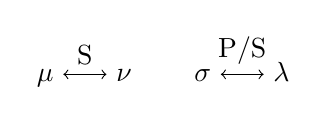
\begin{tikzpicture}

\snode{MU}{0,0}{\mu};
\snode{NU}{1,0}{\nu};
\snode{SIG}{2,0}{\sigma};
\snode{LAM}{3,0}{\lambda};

\draw[<->] (MU) -- (NU) node [midway, above] () {S};
\draw[<->] (SIG) -- (LAM) node [midway, above] () {P/S};

\end{tikzpicture}
\end{center}

\noindent The counstruction of $\mathbf{J}$ has an inherent compuational complexity of $\ccpx{2}$, eventhough the number of non-zero elements scales linearly due to the overlap relationship between $\mu$ and $\nu$. Quadratic scaling algorithms are straight-forward to implement. The first method to construct $\mathbf{J}$ with $\mathcal{O}(N)$ effort was the continous fast multipole method (CFMM, cf Section .). For each element $\mu\nu$ the contributions $\sigma\lambda$ are split into near-field and far-field contributions. NF interactions are computed using standard integration techniques, while FF interactions are computed using multi-level multipole expansion. The linear scaling consists even if the density matrix is not sparse. Other tree-like algorithms have also been proposed (Str1996,Cha1996). In all cases, computing the NF interactions are by far the most time-consuming step.

? J-engine ?

To speed up the evaluation of the non-classical contributions, one may introduce the density fitting approximation (Eq. ...). The coulomb matrix is then evaluated in several steps via an intermediate $\mathbf{d}$ as 
\begin{equation}
J_{\mu\nu} = \cn{\mu\nu}{X} \tilde{d}_X
\end{equation}
\begin{equation}
d_X = \cn{Y}{\mu\nu} P_{\nu\mu} ; \quad \tilde{d}_X = \cn{X}{Y}^{-1} d_X 
\end{equation}
\noindent The computational effort remains unchanged, with $\ccpx{2}$, but with a much lower prefactor, especially for larger, more diffuse basis sets (ref Weigend). The inversion of the metric matrix $\cn{X}{Y}$ scales cubically, and dominates the cost of the DF approximation for large molecules. 

For long-range interactions, one could also consider using local density fitting, such as the atomic resolution of the idenstity or pair-atomic reslution of the identity. Unfortunately, LDF also only reduces the prefactor, rather than scaling. Furthermore, it is necessary to use the robust density fitting of the electron integrals (Eqaution ...) to recover quadratic scaling in the fitting error, due to the constraints imposed on the density fitting procedure. The coulomb matrix is then expressed as
\begin{equation}
J_{\mu\nu} = \cn{\mu\nu}{X} b_X + c^Y_{\mu\nu} \left[ g_Y - \tilde{g}_Y \right]
\end{equation}
\begin{equation}
g_X = C^X_{\mu\nu} P_{\mu\nu}; \quad \tilde{g}_X = \cn{X}{Y} b_{Y}; \quad b_{X} = C_{\mu\nu}^{X} P_{\mu\nu} 
\end{equation}
\noindent The robust LDF-J approximation is evaluated at an effort similar to standard DF-J. The only advantages to LDF in this case pertain to the fitting procedure itself. It is no longer necessary to invert the 2c2e integrals $\cn{X}{Y}$, and the fitting coefficients $C_{\mu\nu}^{X}$ can be evaluated in linear scaling fashion. However, it has been demonstrated that using Dunlap's robust formula in combination with local metrics leads to "attractive electron" states where the SCF energy may converge to very high positive values (Mer2013,Hol2014). The reason is that the the two-electron integral tensor in the robust LDF approximation is no longer postive semidefinite, but \emph{indefinite}, which can lead to severe convergence problems. One way to circumvent this problem is to loosen the constraints on the density fitting procedure, or use a larger auxiliary basis set. In both cases, performance is compromised.  

As shall be shown in the results section/chapter?, quasi-robust density offers a better alternative to robust LDF-J methods, with high accuracy, and without convergence problems.  

MEMORY : ON-THE FLY

POISSON? 
% MANBY, F. R., and KNOWLES, P. J., 2001,Phys.  Rev.Lett.,87,163001.
% MANBY, F. R., KNOWLES, P. J., and LLOYD, A. W., 2001,J. Chem. Phys.,115,9144.

% Str1996 Strain MC, Scuseria GE, Frisch MJ. Achieving linear scaling for the electronic quantum coulomb problem. Science 1996, 271:51–53.
% Cha1996 Challacombe M, Schwegler E, Alml ̈of J. Fast assem-bly of the Coulomb matrix: a quantum chemical treecode.J Chem Phys1996, 104:4685
% Mer2013 Merlot, P.; Kjæ rgaard, T.; Helgaker, T.; Lindh, R.; Aquilante,F.; Reine, S.; Pedersen, T. B.J. Comput. Chem.2013,34, 1486−96.
% Hollman, D. S.; Schaefer, H. F.; Valeev, E. F.J. Chem. Phys.2014,140, 064109.

\subsection{The Exchange Matrix}

\subsubsection{Exact Exchange}

The expression for the exchange matrix is given by 
\begin{equation}
K_{\mu\nu} = \cn{\mu\sigma}{\nu\lambda} P_{\lambda\sigma}
\end{equation}
\noindent In the section where sparsity diagrams were introduced, it was demonstrotated that the indices of the exchange expression can be fully linked:
\begin{center}
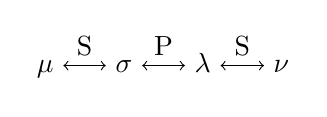
\begin{tikzpicture}

\snode{MU}{0,0}{\mu};
\snode{NU}{3,0}{\nu};
\snode{SIG}{1,0}{\sigma};
\snode{LAM}{2,0}{\lambda};

\draw[<->] (MU) -- (SIG) node [midway, above] () {S};
\draw[<->] (SIG) -- (LAM) node [midway, above] () {P};
\draw[<->] (LAM) -- (NU) node [midway, above] () {S};

\end{tikzpicture}
\end{center}
\noindent The non-zero elements in $\mathbf{K}$ scale linearly and can also be evaluated with $\mathcal{O}(N)$. This property has been realized quite early on (Sch1996). However, a straight-forward implementation where the 4c2e integrals are directly contracted with the density matrix $\mathbf{P}$ using sparse matrix algebra does not give the desired results, when applying the standard $\ccpx{2}$ Schwarz-screening to $\cn{\mu\sigma}{\nu\lambda}$. To lower the scaling of electron integral evaluation, it is important to design a screening algorithm which imposes the P junction between $\sigma$ and $\lambda$ which in turn leads to only a linear increase in the number of bra-ket pairs. 

The ONX method by Schwegler (Sch1997) was the first $\mathcal{O}(N)$ scheme for constructing the exchange matrix, but did not exploit permutational symmetry, which lead to a four fold increase in the prefactor. More competitive methods were proposed later, such as Linear Exchange (LinK) by Ochsenfled et al (Och1997), or symmetrized ONX (SONX) (Sch2000) that could also be applied to small systems without major overhead.

For all approaches, an important step is the screening of the bra-ket pairs using a density-weighted integral estimate
\begin{equation}
|P_{\lambda\sigma}||\cn{\mu\sigma}{\mu\sigma}|^{1/2} |\cn{\nu\lambda}{\nu\lambda}|^{1/2} \leq \tau
\end{equation}
\noindent which scales linearly for increasing size of systems whith large HOMO-LUMO gaps. Furthermore, shell ordering is very important to avoid the $\ccpx{2}$ complexity of thresholding and enable early exit out of the shell loops during contruction of the exchange matrix. Similarly to the J kernel, the electron integrals need not to be held in memory, but can be recomputed on the fly.

% Sch1996 https://aip.scitation.org/doi/10.1063/1.472135
% Sch1997 https://aip.scitation.org/doi/10.1063/1.473833
% Och1998 https://aip.scitation.org/doi/10.1063/1.476741
% Sch2000 https://link.springer.com/article/10.1007%2Fs002140000127

\subsubsection{Density Fitting}

The downside of exact linear exchange algorithms is the steep $\ccpx{4}$ scaling with increasing basis set size which delays the onset of the low-scaling regime. For this reason, considerable effort has been invested in recent years to also exploit rank sparsity by density fitting. The DF expression for the exchange matrix in the AO basis reads
\begin{equation}
C^X_{\mu\nu} = \cn{X}{Y}^{-1} \cn{Y}{\mu\nu}
\end{equation}
\begin{equation}
K_{\mu\nu} = C^X_{\nu\lambda} \cn{X}{\mu \sigma} P_{\sigma\lambda}
\end{equation}
\noindent In a straight-forward implementation using sparse matrix algebra, Equation ... and Equation .. are evaluated with $\ccpx{3}$  and $\ccpx{2}$ effort respectively. The non-zero elements of both the fitting coefficients $C$ and the 3c2e integrals increase quadratically. Their storage can quickly become problematic for large basis sets if both are held in-core. In principle, both tensors can be recomputed batchwise on-the-fly to reduce memory-footprint, but in contrast to the DF-J kernel where only the 3c2e integrals need to be generated at each iteration, recomputing the fitting coefficients each time introduces a prefactor that is too large for an out-of-core DF-K kernel to be of any practical use. 

For an efficient, direct evaluation of the exchange matrix using density fitting, an MO based approach is much more favourable (Wei2002). The MO-DF-K kernel is evaluated as
\begin{equation}
B^{X}_{\mu i} = C_{\nu i} \cn{X}{\mu\nu}
\end{equation} 
\begin{equation}
D^{X}_{\mu i} = \cn{X}{Y}^{-1/2} B^{X}_{\mu i}
\end{equation}
\begin{equation}
K_{\mu\nu} = B^{X}_{\mu i} B^{X}_{\nu i}
\end{equation}
\noindent with cubic computational complexity. The matrix elements of the exchange matrix are evaluated batch-wise over occupied blocks $I$. By contracting the 3c2e electron integrals with the coeffcient matrix $C_{\mu i}$ to form the half-transformed integrals $B^X_{\mu i}$, storage can be reduced from $N_{aux} N_{AO}^2$ to $N_{aux} N_{AO} N_{occ} / N_I$. The 3c2e integrals need to be recomputed for each block $I$, but in practice the number of blocks can be held quite small. The DF-MO-K method is especially well suited for small to medium sized molecules with large diffuse basis sets for post-HF calculations.      

% Wei2002 https://pubs.rsc.org/en/content/articlehtml/2002/cp/b204199p

\subsubsection{Local Density Fitting}

For standard density fitting, one looses the linear scaling character of the exchange matrix, which can however be recovered by using LDF. Again, the Dunlap's robust density fitting needs to applied to get accurate results. The robust DF-K kernel can take the form
\begin{eqnarray}
E_{\mu\nu}^{X} =& C^{X}_{\mu\sigma} P_{\lambda\nu} \\
L_{\mu\nu} =& E_{\mu\sigma}^X \cn{X}{\nu\sigma} - \frac{1}{2} E_{\mu\sigma}^X \cn{X}{Y} C^{Y}_{\nu\sigma} \\
K_{\mu\nu} =& L_{\mu\nu} + L_{\nu\mu}
\end{eqnarray}
\noindent All steps can be evaluated in $\mathcal{O}(N)$ time, if one presumes linear scaling of the fitting coeffcients:
\begin{center}
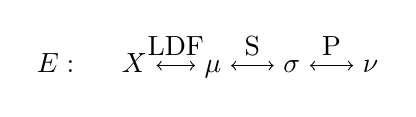
\begin{tikzpicture}
\snode{E}{0,0}{E:};
\snode{X}{1,0}{X};
\snode{MU}{2,0}{\mu};
\snode{SIGMA}{3,0}{\sigma};
\snode{NU}{4,0}{\nu};
\draw[<->] (X) -- (MU) node [midway, above] () {LDF};
\draw[<->] (MU) -- (SIGMA) node [midway, above] () {S};
\draw[<->] (SIGMA) -- (NU) node [midway, above] () {P};
\end{tikzpicture}
\end{center}
\begin{center}
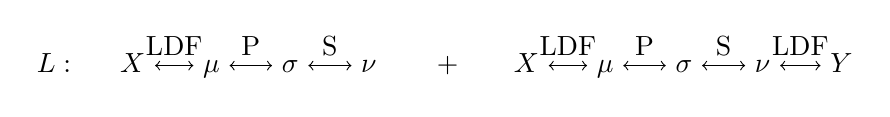
\begin{tikzpicture}
\snode{L}{0,0}{L:};
\snode{X}{1,0}{X};
\snode{MU}{2,0}{\mu};
\snode{SIGMA}{3,0}{\sigma};
\snode{NU}{4,0}{\nu};
\snode{PLUS}{5,0}{+};
\snode{X1}{6,0}{X};
\snode{MU1}{7,0}{\mu};
\snode{SIGMA1}{8,0}{\sigma};
\snode{NU1}{9,0}{\nu};
\snode{Y}{10,0}{Y};
\draw[<->] (X) -- (MU) node [midway, above] () {LDF};
\draw[<->] (MU) -- (SIGMA) node [midway, above] () {P};
\draw[<->] (SIGMA) -- (NU) node [midway, above] () {S};
\draw[<->] (X1) -- (MU1) node [midway, above] () {LDF};
\draw[<->] (MU1) -- (SIGMA1) node [midway, above] () {P};
\draw[<->] (SIGMA1) -- (NU1) node [midway, above] () {S};
\draw[<->] (NU1) -- (Y) node [midway, above] () {LDF};
\end{tikzpicture}
\end{center}
\begin{center}
\begin{tikzpicture}

\snode{K}{0,0}{K:};

\snode{MU}{1,0}{\mu};
\snode{NU}{2,0}{\nu};
\snode{PLUS}{3,0}{+};
\snode{MU1}{5,0}{\nu};
\snode{NU1}{4,0}{\mu};

\draw[<->] (MU) -- (NU) node [midway, above] () {};
\draw[<->] (NU1) -- (MU1) node [midway, above] () {};
\end{tikzpicture}
\end{center}

\noindent Alternatively, an LDF-K scheme based on LMOs is also possible (Pol2004,Mej2014). Over the years, many different LDF-K kernels have been proposed that approximate $C_{\mu\nu}^X$ based on LMO domains (Pol2004,Mej2014), the atomic resolution of the identity (ARI) (Sod2007), the pair-atomic resolution of the identity (PARI) (Mer2013) or the concentric atomic density fitting (CADF) (Hol2017). Although the electron integrals are no longer positive semidefinite, LDF-K is not plagued by the same convergence problems as LDF-J, and it has been shown that LDF-K can be combined with standard DF-J to circumvent convergence problems (Man2015). 

% Pol2004 https://www.tandfonline.com/doi/abs/10.1080/0026897042000274801
% Sod2007 Hartree-Fock exchange computed using the atomic resolutionof the identity approximation
% Mer2013 https://onlinelibrary.wiley.com/doi/10.1002/jcc.23284
% Mej2014 https://aip.scitation.org/doi/full/10.1063/1.4896199
% Man2015 https://pubs.acs.org/doi/abs/10.1021/ct5008586
% Hol2017 Fast construction of the exchange operator in an atom-centred basis with concentric atomic densityfitting

\subsubsection{Other}

% COS Nee2009 https://www.sciencedirect.com/science/article/pii/S0301010408005089
% COS2 Isz2011 https://aip.scitation.org/doi/full/10.1063/1.3646921
% ADFMM Gui2010 https://pubs.acs.org/doi/10.1021/ct1002225

\subsection{The SCF Procdure}

In the standard SCF procudure, the construction of the Fock matrix is followed by a cubic scaling diagonalization to obtain the MO coefficient matrix and the MO energies. As was discussed in detail in previous sections, the eigenvectors of the Fock matrix, i.e. the canonical MOs, are delocalized, and therefore using a sparse eigenvalue solver is unfortunately not an option. The solution is to entirely avoid any MO quantities and replace the Fock diagonalization step. For a functional, fully AO-based method, the same constraints on the density matrix need to be fulfilled as in the standard SCF procedure:
\begin{equation}
\mathbf{P} = \mathbf{P}^{\dagger} \qquad \textrm{Hermiticity}
\end{equation}
\begin{equation}
Tr(\mathbf{PS}) = N_{ele} \qquad \textrm{N-representability}
\end{equation}
\begin{equation}
\mathbf{PSP} = \mathbf{P} \qquad \textrm{Idempotency}
\end{equation}
\begin{equation}
\mathbf{FPS} - \mathbf{SPF} = \mathbf{0} \qquad \textrm{Commutator}
\end{equation}
\noindent There are two main approaches for replacing Fock matrix diagonalization: Purification (or spectral projection) and density matrix minimzation (Jor2005).

In spectral projection methods, an inital guess for the density matrix $\mathbf{P}$ of its Fock matrix $\mathbf{F}$ is obtained as
\begin{equation}
\mathbf{P} = \Theta \left( \mu \mathbf{I} - \mathbf{F} \right)
\end{equation}
\noindent where $\mu$ is the chemical potential, and $\Theta$ is the Heavyside step-function. The guess density then has orbital occupation numbers spread between 0 and 1, and has the same eigenvectors as the Fock matrix. The idempotent density is then determined by \emph{density purification}. Density purification is a iterative procudre where a purification transformation is repeatedly applied to the density matrix which converges the orbital occupation numbers either towards 0 or 1. One of the earliest purification transformation by McWeeny (Wee1959) takes the form
\begin{equation}
\mathbf{P}_{n+1} = 3\mathbf{P}_n\mathbf{SP}_n - 2\mathbf{P}_n\mathbf{SP}_n\mathbf{SP}_n
\end{equation}
\noindent Equation ... is also known as the grand-canonical purification scheme. Other transformations have been proposed over the years, such as canonical purification (Pal1998) or trace-resetting purification (Nik2003), which do not need the chemical potential $\mu$. The only operations in purification schemes are matrix multiplications, which can be made linearly scaling using sparse matrix algebra. Compared to Fock diagonalization, density purification has a larger overhead, but can be easily integrated without needing large modifications of existing SCF code.

The second method, density matrix minimization, starts from an existing idempotent density matrix guess from a previous SCF cycle and minimizes the energy functional (Li1993,Daw1993,Nun1994)
\begin{equation}
E = Tr\left[ \left(3\mathbf{PSP} - 2\mathbf{PSPSP}\right)\left(\mathbf{K} - \mu \mathbf{I}\right) \right]
\end{equation}
\noindent where $\mathbf{K}$ is the effective one-electron Hamiltonian matrix. The energy minimum is found either by gradient descent or the curvy-step approach (Hel2000,Sha2003).

% Jor2005
% McWeeny R. Hartree–Fock theory with nonorthogo-nal basis functions.Phys Rev1959, 114:1528–1529
% Pal1998 A. H. R. Palser and D. E. Manolopoulos, Phys. Rev. B58, 12704~1998!.
% Nik2003 https://aip.scitation.org/doi/pdf/10.1063/1.1559913
% Li1993 https://journals.aps.org/prb/abstract/10.1103/PhysRevB.47.10891
% Daw1993 https://journals.aps.org/prb/abstract/10.1103/PhysRevB.47.10895
% Nun1994 https://journals.aps.org/prb/abstract/10.1103/PhysRevB.50.17611
% Hel2000 https://journals.aps.org/prb/abstract/10.1103/PhysRevB.50.17611
% Sha2003 https://aip.scitation.org/doi/10.1063/1.1558476

\section{Local Ground State Correlation Methods: MP2}

Second-Order M{\o}ller Plesset is one of the simplest post-Hartree Fock methods available, but still scales as $\ccpx{5}$. Since the seminal work of Saebo and Pulay (Pul1983,Sae1985), several different methods have been proposed which drastically reduce the computational complexity. Attempts can generally be grouped into two categories: AO-MP2 and LMO-MP2. While both schemes do have their differences, they share some of the problems assciated with computing the MP2 energy in a local basis.

First, the energy denominator in the MP2-amplitudes $t$ make it difficult to reformulate the MP2 energy expressions in a different basis. AO-MP2 and LMO-MP2 take different approaches: AO-MP2 solves the problem using the Laplace quadrature, while LMO-MP2 methods usually use an orbital-invariant formulation of MP2 using the Hylleraas functional.

Second, steps involving the transformation of the AO 2-electron integrals to the Pseudo-AO or LMO basis still remain a major bottle-neck, even with sparsity involved. Both AO- and LMO-MP2 use screening criteria, additional domain restrictions, density fitting or similar methods to lower the cost of integral transformation. These additional procedures are crucial if one wishes to achieve a truly linear scaling MP2 method with a reduced overhead.

We will now address each point in detail in the next sections.

\subsection{Atomic Orbital MP2}

MP2 was first formulated in the AO basis in 1993 by Häser , and a linear scaling algorithm was presented by Scuseria and Ayala in 1999 (ref). AO-MP2 has since then been extended to DF-MP2 (ref) and SOS-MP2 (ref). 

ALSO: CC2 CAN ALSO BE USED SIMILARLY

\subsubsection{The Laplace Transform}

In 1991, Almlöf showed (Alm1991) that the energy denominator in the MP2 amplitudes can be removed using an integral transform called the \emph{Laplace Transform}

\begin{equation}
\frac{1}{\eps_a + \eps_b - \eps_i - \eps_j} = \int_0^{\infty} e^{-\left(\eps_a + \eps_b - \eps i - \eps_j\right)t} dt
\end{equation}

The t-integration can be replaced (Has1993) by a finite summation using a functional approximation:

\begin{equation}
\frac{1}{\eps_a + \eps_b - \eps_i - \eps_j} \approx \sum_{\alpha}^{n} w\pa e^{-\left(\eps_a + \eps_b - \eps i - \eps_j\right)t\pa}
\end{equation} 

\noindent where $w\pa$ and $t\pa$ are the Laplace weights and exponents at the Laplace points $\alpha$. Accuracy can be controlled by the number of Laplace points $n$. An efficient AO-MP2 implementation heavily relies on an accurate quadrature scheme to achive the desired accuracy using as few Laplace points as possible to reduce overhead caused by the repeated AO transformation at each step. In general, 5-8 Laplace points are needed to achieve milli-Hartree accuracy, and 10 to 15 points for $\mu$Hartree accuracy. For more details, the reader is referred to section ... .

\subsubsection{AO MP2 Equations}

Using the Laplace transform, the energy expression for restricted canonical MP2 can be expressed as
\begin{equation}
\begin{split}
E_{MP2} &= - \sum_{iajb} \frac{\cn{ia}{jb} \left[2 \cn{ia}{ib} - \cn{ib}{ja} \right]}{\eps_a + \eps_b - \eps_i - \eps_j} \\
&\approx - \sum_{\alpha}^n \sum_{iajb} \cn{ia}{jb} \left[2 \cn{ia}{ib} - \cn{ib}{ja} \right] w\pa e^{-\left(\eps_a + \eps_b - \eps i - \eps_j\right)t\pa}
\end{split}
\end{equation}

\noindent We can then proceed to factor out the coefficient matrices 
\begin{equation}
\begin{split}
&- \sum_{\alpha}^n \sum_{iajb} \cn{ia}{jb} \left[2 \cn{ia}{ib} - \cn{ib}{ja} \right] w\pa e^{-\left(\eps_a + \eps_b - \eps i - \eps_j\right)t\pa} \\
= &- \sum_{\alpha}^n \sum_{iajb} \sum_{\substack{\mu\nu\lambda\sigma \\ \mu'\nu'\lambda'\sigma'} } w\pa e^{-\left(\eps_a + \eps_b - \eps i - \eps_j\right)t\pa} C_{\mu' i} C_{\sigma' a} \cn{\mu'\sigma'}{\nu'\lambda'} C_{\nu' j} C_{\lambda' b} \\ 
 & \qquad \cross \left\lbrace C_{\mu i} C_{\sigma a} \left [ 2\cn{\mu\sigma}{\nu\lambda} -  \cn{\mu\lambda}{\nu\sigma} \right] C_{\nu j} C_{\lambda b} \right\rbrace  \\
= & - \sum_{\alpha}^n \sum_{\substack{\mu\nu\lambda\sigma \\ \mu'\nu'\lambda'\sigma'}} \unl{P}\pa_{\mu\mu'} \ovl{P}\pa_{\sigma\sigma'} \cn{\mu'\sigma'}{\nu'\lambda'} \unl{P}\pa_{\nu\nu'} \ovl{P}\pa_{\lambda\lambda'} \left [ 2\cn{\mu\sigma}{\nu\lambda} -  \cn{\mu\lambda}{\nu\sigma} \right] 
\end{split}
\end{equation}

\noindent with the occupied and virtual \emph{pseudo} or \emph{Laplace} density matrices 
\begin{equation}
\begin{split}
\unl{P}\pa_{\mu\mu'} = \sum_i C_{\mu i} e^{0.25 ln(w\pa) + \eps_i t\pa} C_{\mu' i} \\
\ovl{P}\pa_{\mu\mu'} = \sum_i C_{\sigma a} e^{0.25 ln(w\pa) - \eps_a t\pa} C_{\sigma' i}
\end{split}
\end{equation}

\noindent Introducing the \emph{pseudo-AO} transformed electron integrals
\begin{equation}
\cn{\ulgm\olgs}{\ulgn\olgl}\pa = \unl{P}\pa_{\mu\mu'} \ovl{P}\pa_{\sigma\sigma'} \cn{\mu'\sigma'}{\nu'\lambda'} \unl{P}\pa_{\nu\nu'} \ovl{P}\pa_{\lambda\lambda'}
\end{equation}

\noindent the energy expression for AO-MP2 reads
\begin{equation}
E_{AO-MP2} = - \sum_{\alpha}^n \sum_{\mu\nu\lambda\sigma} \cn{\ulgm\olgs}{\ulgn\olgl}\pa \left [ 2\cn{\mu\sigma}{\nu\lambda} -  \cn{\mu\lambda}{\nu\sigma} \right]
\end{equation}

\noindent For t = 0, $\unl{\mathbf{P}}\pa$ and $\ovl{\mathbf{P}}\pa$ are equal to the Hartree Fock density matrices. The Laplace matrices also fulfill similar relationships
\begin{equation}
\unl{\mathbf{P}}\pa \mathbf{S} \ovl{\mathbf{P}}\pa = \mathbf{0}
\end{equation}
\begin{equation}
\unl{\mathbf{P}}\pa \mathbf{S} + \ovl{\mathbf{P}}\pa \mathbf{S} = \mathbf{I}_{exp}
\end{equation}
\noindent where $\mathbf{I}_{exp}$ is a diagonal matrix with trace
\begin{equation}
Tr[\mathbf{I}_{exp}] = \sum_i e^{0.25 ln(w\pa) + \eps_i t\pa} + \sum_a e^{0.25 ln(w\pa) - \eps_a t\pa}
\end{equation}

The entries of the pseudo-density also decay exponentially as function of the distance between pseudo-AO centres. 

STRICTLY SPEAKING, NOT ENTIRELY IN AN AO BASIS, BUT MIXED AO-pseudo-PAO-basis.

\subsubsection{Quadratic Scaling AO-MP2}

Using the linked index rule, we can easily find the computational complexity of the AO-MP2 method. From the energy expression in Eq. we find that we compute the dot product between two different tensors, the AO-ERIs $\cn{\mu\sigma}{\nu\lambda}$ and the pseudo-AO-ERIs $\cn{\ulgm\olgs}{\ulgn\olgl}\pa$. The scaling is thus determined by the sparsity of those two tensors. We know from a previous discussion that the ERIs can be computed with $\ccpx{2}$ effort. The pseudo-AO ERIs are computed by transforming the ERIs with the pseudo-density matrices, whose indices $\mu,\nu$ are connected by a P junction. The diagrammatic expression for the pseudo-AO ERIs in Eq. ... is given by
\begin{equation}
\begin{split}
\mu \xlr{P} \mu' \xlr{S} \sigma' \xlr{P} \sigma \\
\nu \xlr{P} \nu' \xlr{S} \lambda' \xlr{P} \lambda
\end{split}
\end{equation}

\noindent Two vertices indicate an $\ccpx{2}$ effort for evaluating Eq. ... . Therefore, the inherent asymptotic scaling of AO-MP2, without any other further approximations, is $\ccpx{2}$ as well. Similarly to the AO ERIs, a quadratic scaling evaluation of the pseudo-AO ERIs can be achived using a Schwarz-like screening, as first advocated by Almlöf. Defining the screening matrices

\begin{equation}
\begin{split}
Q_{\mu\nu} &= \mid \cn{\mu\nu}{\mu\nu} \mid ^{1/2} \\
X_{\mu\nu} &= \mid \cn{\ulgm\nu}{\ulgm\nu} \mid ^{1/2} \\
Y_{\mu\nu} &= \mid \cn{\mu\olgn}{\mu\olgn} \mid ^{1/2} \\
Z_{\mu\nu} &= min\left( \sum_{\sigma} A_{\mu\sigma} \mid \ovl{P}_{\sigma\nu} \mid; \sum_{\sigma} B_{\mu \sigma} \mid \unl{P}_{\sigma\nu} \mid \right)
\end{split}
\end{equation} 

\noindent gives an upper-bound for each transformation step in Eq. ..., for example 

\begin{equation}
\cn{\mu'\sigma'}{\nu'\lambda'} \leq Q_{\mu'\sigma'}Q_{\nu'\lambda'}
\end{equation}
\begin{equation}
\cn{\ulgm\sigma'}{\nu'\lambda'} \leq X_{\mu'\sigma'}Q_{\nu'\lambda'}
\end{equation}
\begin{equation}
\cn{\ulgm \olgs}{\ulgn\olgl} \leq Z_{\mu\sigma} Z_{\nu\lambda}
\end{equation}

\noindent and an eficient screening protocol can be devised (Has1993) to get quadratic scaling AO-MP2.

\subsubsection{Linear Scaling AO-MP2}

For the two-electron repulsion integrals, the $1/R$ decay between the charge densities $\cbra{\mu\sigma}$ and $\cket{\nu\lambda}$ is too slow to be of any use even for large systems. However, it has been shown (Aya1999) that $bra$ and $ket$ in the Laplace integral tensor $e\pa$ decays much faster with $1/R^3$. Here, we follow the discussion in Ref Lam2005a. 

For two non-overlapping charge densities $\cbra{\mu\sigma}$ and $\cket{nu\lambda}$ the following inequality holds
\begin{equation}
\cn{\mu\sigma}{\nu\lambda} = \cbra{\mu\sigma}\frac{1}{\mathbf{r}_{12}}\cket{\nu\lambda} \leq \frac{1}{R} \left\lvert \sum_{n=0}^{\infty} \frac{\cbra{\mu\sigma} \left( \mathbf{r}_1 - \mathbf{r}_2 \right)^n \cket{\nu\lambda}}{R^n} \right\rvert
\end{equation}

\noindent We then introduce the following abbreviation for the $n$th order 1-centre multipole integrals
\begin{equation}
M^{(n)}_{\mu\sigma} = \int \chi_{\mu}(r_1) \mathbf{r}_1^n \chi_{\sigma}(r_1) dr
\end{equation}

\noindent where $M^{0}$ are the overlap integrals, $M^{1}$ are the dipole integrals etc. We can then rewrite equation (...) as a multipole expansion
\newcommand{\mpole}[2]{M_{#1}^{(#2)}}
\begin{equation}
\begin{split}
\cn{\mu\sigma}{\nu\lambda} &\leq R^{-1} \left\lvert \mpole{\mu\sigma}{0} \mpole{\nu\lambda}{0} \right\rvert + R^{-2} \left\lvert \mpole{\mu\sigma}{1} \mpole{\nu\lambda}{0} - \mpole{\mu\sigma}{0} \mpole{\nu\lambda}{1} \right\rvert \\
&+ R^{-3} \left\lvert \mpole{\mu\sigma}{2} \mpole{\nu\lambda}{0} - 2 \mpole{\mu\sigma}{1} \mpole{\nu\lambda}{1} + \mpole{\mu\sigma}{0} \mpole{\nu\lambda}{2}\right\rvert \\
&+ R^{-4} \left\lvert \mpole{\mu\sigma}{3} \mpole{\nu\lambda}{0} - 3\mpole{\mu\sigma}{2} \mpole{\nu\lambda}{1} + 3\mpole{\mu\sigma}{1} \mpole{\nu\lambda}{2} - \mpole{\mu\sigma}{0} \mpole{\nu\lambda}{3}\right\rvert \\
&+ \mathcal{O}(R^{-5})
\end{split}
\end{equation}

From equation ..., we know that $M_{\ulgm\olgs}^{(0)} = S_{\ulgm\olgs} = 0$. The multipole expansion for the pseudo-AO ERIs $e\pa$ is therefore reduced to
\begin{equation}
\begin{split}
\cn{\ulgm\olgs}{\ulgn\olgl} &\leq R^{-3} \left\lvert - 2 \mpole{\ulgm\olgs}{1} \mpole{\ulgn\olgl}{1} \right\rvert \\
&+ R^{-4} \left\lvert - 3\mpole{\ulgm\olgs}{2} \mpole{\ulgn\olgl}{1} + 3\mpole{\ulgm\olgs}{1} \mpole{\ulgn\olgl}{2} \right\rvert + \mathcal{O} \\
&+ \mathcal{O}(R^{-5})
\end{split}
\end{equation}

\noindent which shows the $1/R^3$ dependence of the tensor $\cn{\ulgm\olgs}{\ulgn\olgl}$. Combined with the $1/R$ decay of the AO ERIs, this leads to an overall $1/R^4$ behaviour for the AO-MP2 energy. This long-range decay can be exploited to introduce a sparsity relationship between the bra and ket quantities, and reduce the scaling of AO-MP2 from $\ccpx{2}$ to $\ccpx{1}$. In the original paper by Ayala and Scuseria, this decay was accounted for by introducing an interaction domain centred on each atomic orbital $\mu$ in the form of a sphere. For the integrals $\cn{\ulgm\olgm}{\ulgn\olgn}$, the domain $\mathcal{D}(\mu)$, comprises all charge distributions $\sigma\lambda$ for which 
\begin{equation}
\left( \unl{P}_{\mu\sigma} S_{\sigma\lambda} \ovl{P}_{\lambda\mu} \right) \geq \epsilon 
\end{equation}
\noindent The radius $R_{\mu}$ of the interaction sphere is defined by the maximum distance between $\mu$ and the charge density $\sigma\lambda$ in its domain. One can then screen long-range behaviour for the interaction sphere $\mu$ and $\nu$ by the distance criterium
\begin{equation}
r_{\mu\nu} - R_{\mu} - R_{\nu} \geq r_0
\end{equation}
\noindent The biggest drawback of the scheme above is that the thresholding parameters $r_0$ and $\epsilon$ are system-dependent. 
A more rigorous screening method has been proposed by Lambrecht et al. known as multipole based integral estimates (MBIE) (Lam2005,Lam2005a). MBIEs offer a tight upper bound for the AO and pseudo-AO electron integrals by using the multipole expansion in Eq. ... and replacing the higher order terms $\mathcal{O}(R^{-5})$ by lower-order ones. 
ALternative: QQR screening

% Pul1983 P. Pulay,Chem. Phys. Lett., 1983,100, 151.27 S. 
% Sae1985 Saebø and P. Pulay,Chem. Phys. Lett., 1985,113, 13
% Alm1991 J. Almlo ̈f, Chem. Phys. Lett.181, 319~1991!
% Has1992 https://aip.scitation.org/doi/abs/10.1063/1.462485
% Has1993 https://link.springer.com/article/10.1007%2FBF01113535
% Aya1999 https://aip.scitation.org/doi/pdf/10.1063/1.478256
% First MBIE Paper: Lam2005 https://aip.scitation.org/doi/pdf/10.1063/1.2079967
% Second MBIE Paper: Lam2005a https://aip.scitation.org/doi/pdf/10.1063/1.2079987
% Improved MBIE Paper: Lam2008 https://pubs.rsc.org/en/content/articlepdf/2008/cp/b804110e

\subsubsection{Cholesky Decomposition of Pseudo-Densities}

As with any method formulated entirely in an AO basis, AO-MP2 suffers from $\ccpx{4}$ scaling with increasing basis set $N$. The cost associated with larger basis sets can be mitigated by Cholesky decomposition of the pseudo-density matrices (CDD) (Zie2009). Similar to the orbital localization technique described in Section ..., where the (incomplete) CD of the occupied and virtual Hartree Fock density matrices yields a set of occupied and virtual Cholesky molecular orbitals, the CD of the pseudo-density matrices $\unl{P}\pa$ and $\ovl{P}\pa$ yields a set of Cholesky pseudo-molecular orbitals: 
\begin{equation}
\mathbf{\unl{P}}\pa = \mathbf{\unl{L}}\pa \mathbf{\unl{L}}^{(\alpha)T}
\end{equation}
\begin{equation}
\mathbf{\ovl{P}}\pa = \mathbf{\ovl{L}}\pa \mathbf{\ovl{L}}^{(\alpha)T}
\end{equation} 
\noindent The pseudo-molecular orbitals show a local behaviour inherited from the sparsity of the pseudo-density matrices. It has been observed however (Lue2017), that the pseudo-MOs $L$ are not always very well localized. A more localized set of MOs can be obtained by using the orthogonalized pseudo-density matrices, for example in the case of $\mathbf{\unl{P}}\pa$:
\begin{equation}
\mathbf{\unl{P}}\pa_{orth} = \mathbf{S}^{1/2} \mathbf{\unl{P}}\pa \mathbf{S}^{1/2}
\end{equation}
\noindent The pseudo-MO coefficients are then obtained as
\begin{equation}
\unl{L}\pa = \mathbf{S}^{-1/2} \mathbf{\unl{L}}\pa_{orth}
\end{equation}
\noindent The square root and inverse square root of the overlap matrix $\mathbf{S}$ are most reliably found by cholesky decomposition. The number of occupied and virtual pseudo-MOs is given by the rank of the occupied/virtual pseudo-density matrices, which in turn is equal or less than the number of occupied/virtual CMOs. 

One can then formulate the CDD-AO-MP2 energy expression
\begin{equation}
E_{CDD-AO-MP2} = - \sum_{\alpha}^n \sum_{\uli\ola\ulj\olb} \cn{\uli\ola}{\ulj\olb}\pa \left [ 2\cn{\uli\ola}{\ulj\olb}\pa -  \cn{\uli\olb}{\ulj\ola}\pa \right]
\end{equation}
\noindent whith the pseudo-MO integrals
\begin{equation}
\cn{\uli\ola}{\ulj\olb}\pa = \unl{L}\pa_{\mu\uli} \ovl{L}\pa_{\sigma\ola} \cn{\mu\sigma}{\nu\lambda} \unl{L}\pa_{\nu\ulj} \ovl{L}\pa_{\lambda\olb}
\end{equation}
\noindent CDD-AO-MP2 therefore reduces the sizes of the tensors from $N^{4}_{AO}$ to $N_{occ}^2N_{vir}^2$, while still being sparse. Similar to AO-MP2, Schwarz screening and interaction domain can be introduced to obtain quadratic and linear scaling CDD-AO-MP2.

% first appearence of CDD-MP2 Zie2009 https://aip.scitation.org/doi/pdf/10.1063/1.3142592
% AO-RPA Lue2017 https://pubs.acs.org/doi/abs/10.1021/acs.jctc.6b01235

\subsubsection{Density Fitting in AO-MP2}

To reduce the prefactor associated with integral transformation, either from AOs to pseudo-AOs, or from AOs to pseudo-MOs, on can furthermore introduce density fitting (Zie2009,Mau2014).The transformed 3c2e integrals are given at each Laplace point $\alpha$ by
\begin{equation}
\cn{X}{\ulgm\olgn}\pa = \cn{X}{\mu'\nu'} \unl{P}\pa_{\mu\mu'} \ovl{P}\pa_{\nu\nu'}  
\end{equation}
\noindent which are evaluated with $\ccpx{2}$ cost. Using local density fitting approxaimations, this step can be reduced to linear. 

\subsubsection{SOS-AO-DF-MP2}

From section ..., we know that SOS-MP2 is a cost-efficient variant of MP2 with excellent accuracy. Starting from equation ..., we omit the same-spin contributions and also apply the density fitting approximation to arrive at the energy expression for the AO-DF-SOS-MP2 (Mau2014,Gla2020)
\begin{equation}
\begin{split}
E_{AO-DF-SOS-MP2} &= - c_{os} \sum^{nlap}_{\alpha=1} \sum_{\mu\nu\sigma\lambda} \cn{\ulgn\olgs}{X}\pa \cn{X}{Y}^{-1} \cn{Y}{\ulgn\olgl}\pa \\
& \cn{\mu\sigma}{X'} \cn{X'}{Y'} \cn{Y'}{\nu\lambda}
\end{split}
\end{equation}
\noindent Introducing the intermediates
\begin{equation}
Z\pa_{XY} = \cn{X}{\ulgm\olgs}\pa \cn{\mu\sigma}{Y}
\end{equation}
\begin{equation}
\tilde{Z}\pa_{XY} = \cn{X}{R}^{-1} Z\pa_{RX}
\end{equation}
\noindent we arrive at a very compact expression
\begin{equation}
E_{AO-DF-SOS-MP2} = - c_{os} \sum^{nlap}_{\alpha=1} \sum_{XY} \tilde{Z}\pa_{XY} \tilde{Z}\pa_{YX} 
\end{equation}
\noindent Without local density fitting, the time determining step is the computation of $\mathbf{Z}\pa$ The sparse map of the intermediate is given by 
%\begin{equation}
%\tikzmark{X}X \quad \mu \xlr{P} \tikzmark{MUP}\mu' \xlr{S} \nu' \xlr{P} \nu; \quad Y 
%\end{equation}
%\begin{tikzpicture}[overlay,remember picture]
%\node (b) at ($(X)!0.5!(MUP)$) {};
%\draw let \p{1}=(b) in node (c) at (\x1,-0.5) {c}; 
%\draw[->,black] (X.south) |- (c.south) -| (MUP.south) ;
%\end{tikzpicture}
\begin{center}
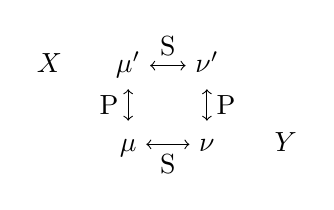
\begin{tikzpicture}

\snode{X}{-1,0}{X};

\snode{MUP}{0,0}{\mu'};
\snode{MU}{0,-1}{\mu};

\snode{NUP}{1,0}{\nu'};
\snode{NU}{1,-1}{\nu};

\snode{Y}{2,-1}{Y};

\draw[<->] (MUP) -- (MU) node [midway, left] () {P};
\draw[<->] (NUP) -- (NU) node [midway, right] () {P};
\draw[<->] (MU) -- (NU) node [midway, below] () {S};
\draw[<->] (MUP) -- (NUP) node [midway, above] () {S};

\end{tikzpicture}
\end{center}
\noindent which suggests that the AO-DF-SOS-MP2 has an overall asymptotic scaling of $\ccpx{3}$. With local density fitting, the graph can however become fully connected
\begin{center}
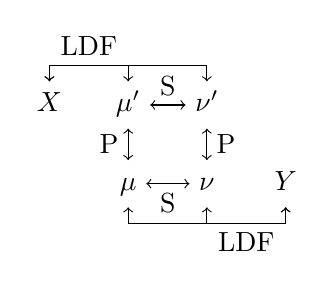
\begin{tikzpicture}

\snode{X}{-1,0}{X};

\snode{MUP}{0,0}{\mu'};
\snode{MU}{0,-1}{\mu};

\snode{NUP}{1,0}{\nu'};
\snode{NU}{1,-1}{\nu};

\snode{Y}{2,-1}{Y};

\draw[<->] (MUP) -- (MU) node [midway, left] () {P};
\draw[<->] (NUP) -- (NU) node [midway, right] () {P};
\draw[<->] (MU) -- (NU) node [midway, below] () {S};
\draw[<->] (MUP) -- (NUP) node [midway, above] () {S};

\draw[<->] (X.north) |- (-0.5,0.5) node[above] {LDF} -| (MUP.north);
\draw[<->] (X.north) |- (-0.5,0.5) node[above] {} -| (NUP.north);

\draw[<->] (Y.south) |- (1.5,-1.5) node[below] {LDF} -| (MU.south);
\draw[<->] (Y.south) |- (1.5,-1.5) node[below] {} -| (NU.south);

\end{tikzpicture}
\end{center}

\noindent where "LDF" is the sparsity relationship introduced between the auxiliary density $X$ and the product density $\cbra{\mu\nu}$, which is metric-specific. In the case of quasi-robust density fitting, LDF = S, and the intermediates $\mathbf{Z}\pa$ can be constructed with linear effort. For weaker decay behaviour, such as the error function coulomb-attenuated metric, the scaling is intermediate between linear and quadratic (Gla2020). 

CAN BE APPLIED TO CC2

% Mau2014 https://aip.scitation.org/doi/full/10.1063/1.4881144
% Gla2020 https://pubs.acs.org/doi/abs/10.1021/acs.jctc.0c00600

% QQR screeening:
% S. A. Maurer, D. S. Lambrecht, D. Flaig, and C. Ochsenfeld, J. Chem. Phys. 136, 144107 (2012). https://doi.org/10.1063/1.3693908
%  S. A. Maurer, D. S. Lambrecht, J. Kussmann, and C. Ochsenfeld, J. Chem. Phys. 138, 014101 (2013). https://doi.org/10.1063/1.4770502

\subsection{Local Molecular Orbital MP2}

Problems with PAO based methods: %NJ Russ, TD Crawford J. Chem. Phys., 2004, 121, 691

While linear scaling MP2 was first achived using an atomic orbital formulation, the first low-scaling MP2 implementations were actually formulated in a local molecular orbital basis with domain-specific virtual orbitals (Pul1983-Sae1987). SEPA, electron pairs etc, NESBETS theorem ....

% Pul1983 https://www.sciencedirect.com/science/article/pii/0009261483807039?via%3Dihub
% Sae1985 https://www.sciencedirect.com/science/article/pii/000926148585003X
% Pul1986 https://link.springer.com/article/10.1007/BF00526697 (ORBITAL INVARIANT)
% Sae1987 https://aip.scitation.org/doi/abs/10.1063/1.452293
% Sae1988 https://aip.scitation.org/doi/abs/10.1063/1.454111

\subsubsection{Laplace LMP2}

In the local molecular orbital basis, the Fock matrix is no longer diagonal, and the amplitudes $t_{ia}^{jb}$ can no longer be easily expressed in a local basis, due to the energy denominator. AO-MP2 tackle this problem by virtue of the Laplace transform. Similarly, one can obtain an energy expression in the LMO basis. The Laplace decomposed MP2 energy is given by
\begin{equation}
E_{MP2} = \sum_{\alpha}^{n} \sum_{iajb} |w\pa| e^{(\eps_i + \eps_j - \eps_a - \eps_j)t\pa} \left[2\cn{ia}{jb} - \cn{ib}{ja}\right] \cn{ia}{jb}  
\end{equation}
\noindent Introducing the unitary occupied and virtual LMO-MO transformation matrix $\mathbf{U}$ 
\begin{equation}
\ket{i} = U_{i\uli} \ket{\uli}
\end{equation} 
\begin{equation}
\ket{a} = U_{i\ola} \ket{\ola}
\end{equation}
\noindent which is factorized out, Equation ... becomes
\begin{equation}
\begin{split}
E_{MP2} &= \sum_{\alpha}^{n} \sum_{iajb} \sum_{\uli\ola\olb} \sum_{\ulk\olc\ull\old} |w\pa| e^{(\eps_i + \eps_j - \eps_a - \eps_j)t\pa} U_{i\uli} U_{a\ola} \left[2\cn{\uli\ola}{\ulj\olb} - \cn{\ulj\olb}{\ulj\olb}\right] U_{j\ulj} U_{b\olb} \\
& \qquad \qquad U_{i\ulk} U_{a\olc} \cn{\ulk\olc}{\ull\old} U_{j\ull} U_{b\old} \\  
&= \sum_{\alpha}^{n} \sum_{\uli\ola\olb} \left[2\cn{\uli\ola}{\ulj\olb} - \cn{\ulj\olb}{\ulj\olb}\right] \sum_{\ulk\olc\ull\old} X_{\uli\ulk}\pa Y_{\ola\olc}\pa \cn{\ulk\olc}{\ull\old} X_{\ulj\ull}\pa Y_{\olb\old}\pa \\
&= \sum_{\uli\ola\olb} \left[2\cn{\uli\ola}{\ulj\olb} - \cn{\ulj\olb}{\ulj\olb}\right] \mathcal{T}_{\uli\ola\ulj\olb}
\end{split}
\end{equation}
\noindent with the Laplace amplitudes $\mathcal{T}$ and the Laplace matrices
\begin{equation}
X_{\uli\ulk}\pa = \sum_i U_{i\uli} |w\pa|^{1/4} e^{\eps_i t\pa} U_{k\ulk}
\end{equation}
\begin{equation}
Y_{\ola\olc}\pa = \sum_a U_{a\ola} |w\pa|^{1/4} e^{-\eps_a t\pa} U_{c\olc}
\end{equation}
\noindent Equation ... is the general expression for the MP2 energy in a local molecular orbital basis, where both the occupied and virtual orbitals are \emph{orthogonal}. The situation changes slightly when using non-orthogonal PAOs, as PAOs and CMOs are no longer related by a unitary transformation:
\begin{equation}
\ket{I} = P_{Ii} \ket{i}
\end{equation} 
\begin{equation}
\ket{i} = P_{Ii} S_{IJ}^{-1} \ket{J} 
\end{equation}
\noindent with $\mathbf{S}$ being the overlap matrix in the PAO basis. Due to the non-orthogonality of the PAOs, entries in the overlap matrix can become very small which might lead to numerical instability when computing its inverse. For this reason, the inverse $\mathbf{S}^{-1}$ is substituted by a more general \emph{pseudo-inverse} $\mathbf{V}$ with the property (see ...)
\begin{equation}
\mathbf{SVS} = V
\end{equation}
\noindent The Laplace matrices will then take the following form instead (Kat2008)
\begin{equation}
\mathbf{X}\pa = \mathbf{V} \mathbf{A}\pa \mathbf{V} \pdg 
\end{equation}
\begin{equation}
\mathbf{Y}\pa = \mathbf{V} \mathbf{B}\pa \mathbf{V} \pdg 
\end{equation}
\begin{equation}
A_{IK}\pa = \sum_i P_{Ii} |w\pa|^{1/4} e^{\eps_i t\pa} P_{kK}
\end{equation}
\begin{equation}
B_{AB}\pa = \sum_a Q_{Aa} |w\pa|^{1/4} e^{-\eps_a t\pa} Q_{Aa}
\end{equation}
\noindent In practice, only the virtual orbital space is transformed to PAOs, while the occupied space is kept in an orthogonal local orbital representation.


% Kat2008 https://pubs.rsc.org/en/content/articlepdf/2008/cp/b802993h

NESBETS THEOREM

\subsubsection{Orbital Invariant MP2}

Alternatively, the local MP2 amplitudes can be determined iteratively via an \emph{orbital-invariant} formulation of the MP2 energy expression. Orbital-invariant MP2 predates LT-MP2 by a decade and is based on the \emph{Hylleraas functional} (Hyl,Pul1986). The  Hylleraas functional form of the energy is given by minimizing 
\begin{equation}
E^{(2)} = min \left[ 2\bra{\Psi^{(1)}} \mathbf{H} - E_0  \ket{Psi^{(0}} - \bra{\Psi^{(1)}} \mathbf{H}_0 - E_0 \ket{\Psi^{(1)}} \right]
\end{equation}
\noindent In the case of MP2, the qunatities in Equation ... take the form
\begin{equation}
\bra{\Psi^{(1)}} \mathbf{H} - E_0  \ket{\Psi^{(0}} = \frac{1}{4} \sum_{ijab} t_{ijab} \bra{ij}\ket{ab}
\end{equation}
\begin{equation}
\bra{\Psi^{(1)}} \mathbf{H}_0 - E_0 \ket{\Psi^{(1)}} = \frac{1}{8} \sum_{ijabc} t_{iajb} f_{cb} t_{iajc} - \frac{1}{8} \sum_{ijkab} t_{iajb} f_{jk} t_{iakb}
\end{equation}
\noindent Minimization of the MP2 Hylleraas functional, with respect to the amplitudes $\mathbf{t}$ yields a set of linear equations given by
\begin{equation}
\begin{split}
R_{iajb} = \bra{ij} {} \ket{ab} + \sum_c \left(t_{ijab} f_{cb} + f_{ac} t_{iacb} \right) - \sum_k \left( t_{iakb} f_{kj} + f_{ik} t_{kajb} \right) = 0
\end{split}
\end{equation}
\noindent where $\mathbf{R}$ is the residual. The amplitudes $\mathbf{t}$ are then no longer computed directly by a closed expresion, but iteratively by solving the system of equations, in a similar vein to coupled cluster. This method is said to be orbital invariant, because any molecular orbital representation can be used. For a set of orthogonal MOs $\uli$ and $\ola$, the quantities in Equation ... are simply replaced by their local equivalent. As was the case in LT-LMP2, if PAOs are to be used for the virtual orbital space, the non-orthogonality needs to be taken into consideration. For a mixed LMO-PAO basis, Equation ... reads
\begin{equation}
\begin{split}
R_{\uli A \ulj B} = & \bra{\uli\ulj}{}\ket{AB} + \sum_C \left( f_{AC} t_{\uli C \ulj L} S_{L B} + S_{AC} t_{\uli C \ulj D} f_{DB} \right) \\
&-  \sum_{\ulk} \left( f_{\uli \ulk} S_{AC} t_{\ulk C \ulj D} S_{D B} + f_{\ulk \ulj} S_{AC} t_{\uli C \ulj D} S_{DB} \right) = 0
\end{split} 
\end{equation}
\noindent For specific virtual orbitals, the equations are solved individually for each electron pair $ij$ to obtain their amplitude $\mathbf{t}_{ij}$ and then compute the pair correlation energy. 

why not AO?

\subsubsection{Quadratic Scaling LMP2}

Similar to CEPA, the MP2 energy can be computed as a sum of electron pair energies
\begin{equation}
E_{MP2} = \sum_ij e_{ij}
\end{equation}
\begin{equation}
e_{ij} = \left( 2t_{ij}^{ab} - t_{ij}^{ba} \right) \cn{ia}{jb} 
\end{equation}
\noindent where the amplitudes $t_{ijab}$ are computed according to Eq. ... . The occupied molecular orbitals $ij$ are localized using e.g. Foster-Boys, Pipiek-Mezey or a Cholesky decomposition of the density matrix. Virtual orbitals are generally localized by projection onto the atomic orbital space (PAOs) and subsequently assigning them to pair domains $[ij]$ (domain specific virtuals), or by diagonalizing the MP2 density matrix for each electron pair (pair natural orbitals).  In all cases, the number of SVOs scales as $\mathbf{O}(1)$ for each electron pair $ij$, in the limit of large molecules (see ...). 
 
For well localized orbitals, the electron pair correlation $e_{ij}$ decays with $1/r_{ij}^6$ whith the distance between orbital centres. Electron pairs are generally divided into four groups: strong pairs ($r_{ij} < 1a_0$), weak pairs ($1 < r_{ij} \leq 8 a_0$), distant pairs ($8 < r_{ij} \leq 15 a_0$), and very distant pairs ($15 < r_{ij}$) (Sch1999). Other than by distance criteria, electron pairs can also be grouped by their pair energy (Nee2009). Figure ... shoes the number of significant electron pairs in each category for glycine chains. The number of strong, weak and distant pairs scale as $\mathcal{O}(N)$, while the number of very distant pairs scales quadratically. 

The major bottle-neck in LMP2 is, as usual, the transformation of the 2 electron integrals from the AO basis into the local basis
\begin{equation}
\cn{\uli\ola}{\ulj\olb} = L_{\mu \uli} L_{\sigma \ola} \cn{\mu\sigma}{\nu\lambda} L_{\nu \ulj} L_{\lambda \olb}
\end{equation}
\noindent The expression above translates into the sparsity diagram
\begin{center}
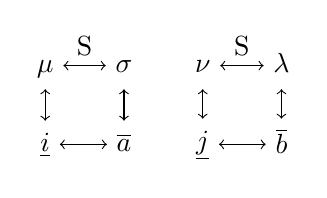
\begin{tikzpicture}

\snode{MU}{0,0}{\mu};
\snode{SIG}{1,0}{\sigma};
\snode{NU}{2,0}{\nu};
\snode{LAM}{3,0}{\lambda};

\snode{I}{0,-1}{\uli};
\snode{A}{1,-1}{\ola};
\snode{J}{2,-1}{\ulj};
\snode{B}{3,-1}{\olb};

\draw[<->] (MU) -- (SIG) node [midway, above] () {S};
\draw[<->] (NU) -- (LAM) node [midway, above] () {S};
\draw[<->] (I) -- (MU) node [midway, below] () {};
\draw[<->] (A) -- (SIG) node [midway, below] () {};
\draw[<->] (J) -- (NU) node [midway, below] () {};
\draw[<->] (B) -- (LAM) node [midway, below] () {};
\draw[<->] (I) -- (A) node [midway, below] () {};
\draw[<->] (J) -- (B) node [midway, below] () {};

\end{tikzpicture}
\end{center}
\noindent which indicates that the MO integrals can be evaluated with $\ccpx{2}$ effort without further approximations. One thing to note is that the quadratic scaling is also obatined, even if the sparsity relationships $i \leftrightarrow a$ and $j \leftrightarrow b$ did not exist, i.e. where virtual orbitals are localized, but not grouped into (apir) domains. The major disadavantage of such non-pair specific methods is that the virtual orbital space is less compact, which leads to a high overhead for integral transformation involving virtual orbitals, which could be the reason that there are no examples in literature using such a scheme. Establishing an a priori sparsity relationship between occupied and virtual space allows to more easily reach the low-scaling regime. 

\begin{figure}
\centering
\includegraphics[scale=0.5]{Pics/electron_pairs.png}
\caption{Taken from Sch1999}
\end{figure}

\subsubsection{Linear Scaling LMP2}

It has been found [Sae1987] early on that the quadratic scaling very distant electron pairs can safely ignored without major impact on the total correlation energy. (Distance or Connectivity ciriteria) Distant pairs can also be approximated either by a multipole expansion (Het1998) or empirically (Rau1995), which further lowers the prefactor of the method. As a consequence, this establishes a sparsity relationship between $i$ and $j$, and the sparsity diagram for the MO integrals becomes fully connected
\begin{center}
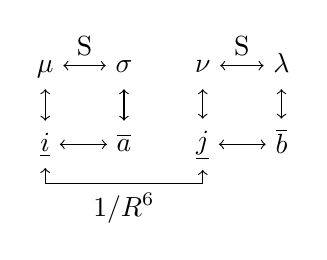
\begin{tikzpicture}

\snode{MU}{0,0}{\mu};
\snode{SIG}{1,0}{\sigma};
\snode{NU}{2,0}{\nu};
\snode{LAM}{3,0}{\lambda};

\snode{I}{0,-1}{\uli};
\snode{A}{1,-1}{\ola};
\snode{J}{2,-1}{\ulj};
\snode{B}{3,-1}{\olb};

\draw[<->] (MU) -- (SIG) node [midway, above] () {S};
\draw[<->] (NU) -- (LAM) node [midway, above] () {S};
\draw[<->] (I) -- (MU) node [midway, below] () {};
\draw[<->] (A) -- (SIG) node [midway, below] () {};
\draw[<->] (J) -- (NU) node [midway, below] () {};
\draw[<->] (B) -- (LAM) node [midway, below] () {};
\draw[<->] (I) -- (A) node [midway, below] () {};
\draw[<->] (J) -- (B) node [midway, below] () {};
\draw[<->] (I) |- (1,-1.5) node [below] {$1/R^6$} -| (J);

\end{tikzpicture}
\end{center}
\noindent and linear scaling LMP2 therefore becomes possible (Sch1999).

% Sch1999 https://aip.scitation.org/doi/pdf/10.1063/1.479957

% distant pairs multipole approximate very distant pairs by multipole expansion Het1998 https://www.sciencedirect.com/science/article/pii/S0009261498004916

% distant pairs Empirically Rau1995 G. Rauhut, J. W. Boughton, and P. Pulay, J. Chem. Phys., 103, 5662 1995 .

Instead of using distance criteria, can use screening: 
%https://aip.scitation.org/doi/10.1063/1.4773581

\subsubsection{Density Fitting for LMP2}

While specific virtual orbitals form a very compact representation of the virtual space, the fact that each electron pair has their own orthogonal vitual orbital basis means that the total number of virtuals can become exceedingly large, and consequently increases the cost associated with the AO-MO transformation step. The most expensive step then becomes
\begin{equation}
\cn{\uli\ola}{P} = L_{\mu\uli} \cn{\mu\nu}{P} L_{\nu\ola}
\end{equation}
\noindent Transformation of the 3c2e integrals scales with $\ccpx{2}$. Linear scaling can be achieved by instroducing an orbital-specific fitting domain $[i]_fit$, e.g. by assigning all auxiliary functions $P$ on atoms with a Mulliken charge above a given threshold for the local orbital $i$ (Pin2015), or by using a Boughton-Pulay like scheme (Wer2015). This yields the sparsity diagramm
\begin{center}
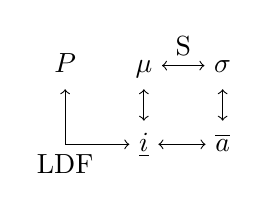
\begin{tikzpicture}

\snode{P}{-1,0}{P};
\snode{MU}{0,0}{\mu};
\snode{SIG}{1,0}{\sigma};

\snode{I}{0,-1}{\uli};
\snode{A}{1,-1}{\ola};

\draw[<->] (MU) -- (SIG) node [midway, above] () {S};
\draw[<->] (I) -- (MU) node [midway, below] () {};
\draw[<->] (A) -- (SIG) node [midway, below] () {};
\draw[<->] (I) -- (A) node [midway, below] () {};
\draw[<->] (I) -- (-1,-1) node [below] {LDF} -- (P);

\end{tikzpicture}
\end{center}
\noindent As opposed to SOS-AO-MP2, where density fitting can give a more favourable factorization of the energy expression, the MO integrals need to fully assembled for LMP2 in order to solve the linear equations (...). The assembly is done in two steps
\begin{equation}
B^{X}_{\uli\ola} = \sum_{Y \in [i]_{fit} \cup [j]_{fit}} \cn{X}{Y}^{-1/2} \cn{Y}{\uli\ola}
\end{equation}
\begin{equation}
\cn{\uli\ola}{\ulj\olb} = \sum_{X \in [i]_{fit} \cup [j]_{fit}} B^{X}_{\uli\ola} B^{X}_{\ulj\olb} 
\end{equation}
\noindent The two steps are repeated for each electron pair $ij$, and the sum runs over all auxiliary functions $P$ in the unified fitting domain $[i]_{fit} \cup [j]_{fit}$, which enforces linear scaling for these steps as well. 

% Pin2015 https://aip.scitation.org/doi/pdf/10.1063/1.4926879
% Wer2015 https://pubs.acs.org/doi/pdf/10.1021/ct500725e

\subsection{Atomic Orbital CC2}

The atomic orbital approach for low scaling MP2 can be extended to CC2 ... currently under work

\subsection{Atomic Orbital CCSD: PAO or AO?}

!!!!!!!!!!!!! REWRITE !!!!!!!!!!!!!!!!
As opposed to MP2 and CC2, where the energy denominator in the closed form expression for the doubles amplitudes $t_{iajb}$ makes it difficult to find an orbital-invariant representation of the energy expressions, it is much easier to do so for CCSD. The restricted CCSD correlation energy expression reads
\begin{equation}
E_{corr} = \sum_{ijab} v_{iajb} t^{CCSD}_{iajb} \qquad v_{iajb} = 2\cn{ia}{jb} - \cn{ib}{ja} 
\end{equation}   
\noindent In their 1999 paper [ref], Scuseria and Ayala have shown that there are two possible "AO" representations of the CCSD correlation energy. The first and most straight-forward approach is to factor out the MO coefficient matrices from the MO electron repulsion integrals $v$, similar to AO-MP2
\begin{equation}
\begin{split}
E_{corr} &= \sum_{ijab} \sum_{\mu\nu\sigma\lambda} C_{\mu i} C_{\sigma  a} v_{\mu\sigma\nu\lambda} C_{\nu j} C_{\lambda b} t_{iajb} \\
&= \sum_{\mu\nu\sigma\lambda} v_{\mu\sigma\nu\lambda} t_{\ulgm\olgs\ulgn\olgl}
\end{split} 
\end{equation}
\noindent whith the amplitudes $\mathbf{t}$ recast in a PAO-like basis:
\begin{equation}
t_{\ulgm\olgs\ulgn\olgl} = C_{\mu i} C_{\sigma a} t_{iajb} C_{\nu j} C_{\lambda b}
\end{equation}
\noindent The MO amplitudes can be recovered with
\begin{equation}
t_{iajb} = \ovl{C}_{\mu i} \ovl{C}_{\sigma a} t_{\ulgm\olgs\ulgn\olgl} \ovl{C}_{\nu j} \ovl{C}_{\lambda b}
\end{equation}
\noindent It should be noted that $\ulgm$, $\olgs$, $\ulgn$ and $\olgl$ do not correspond to the definition of PAOs given in Section .... As opposed to standard PAOs, they lack the overlap matrix $\mathbf{S}$ in the MO-PAO transformation and vice-versa (compare Equation ... with Eqaution ...). Here, the occupied and virtual PAO-like spaces are not mutually orthogonal, but related through the overlap matrix, similar to the pseudo-PAOs used in AO-MP2
\begin{equation}
\mathbf{PSQ} = \mathbf{0} \qquad \mbf{P} + \mbf{Q} = \mbf{S}^{-1}
\end{equation}
\noindent This alternative PAO-like formulation will be referred to as \emph{mutually non-orthogonal projected atomic orbitals} (or mnoPAOs) from here on out.    

\noindent Instead of using this mnoPAO approach, Scuseria and Ayala proposed an alternative formulation where the coefficient matrices are factored out from the t-amplitudes instead, using the PAO backtransformation \ref{CMO2PAO}:
\begin{equation}
\begin{split}
E_{corr} &= \sum_{ijab} \sum_{\mu\nu\sigma\lambda} v_{iajb} C_{\mu i} C_{\sigma  a} \theta_{\ulgm\olgs\ulgn\olgl} C_{\nu j} C_{\lambda b} \\
&= \sum_{\mu\nu\sigma\lambda} \Pi_{\ulgm\olgs\ulgn\olgl} \theta_{\ulgm\olgs\ulgn\olgl}
\end{split} 
\end{equation}
\noindent The PAO-amplitudes $\theta$ are related to the MO quantities by
\begin{equation}
\theta_{\ulgm\olgs\ulgn\olgl} = \ovl{C}_{\mu i} \ovl{C}_{\sigma a} t_{iajb} \ovl{C}_{\nu j} \ovl{C}_{\lambda b}
\end{equation}
\begin{equation}
t_{iajb} = C_{\mu i} C_{\sigma a} \theta_{\ulgm\olgs\ulgn\olgl} C_{\nu j} C_{\lambda b}
\end{equation}
\noindent The mnoPAO and PAO t-amplitudes are related by
\begin{equation}
\theta_{\ulgm\olgs\ulgn\olgl} = S_{\mu\mu'} S_{\olgs\olgs'} t_{\ulgm'\olgs'\ulgn'\olgl'} S_{\ulgn\ulgn'} S_{\olgl\olgl'}  
\end{equation}
\begin{equation}
\theta_{\ulgm\olgs\ulgn\olgl} = P_{\mu\mu'} P_{\olgs\olgs'} \theta_{\ulgm\olgs\ulgn\olgl} P_{\ulgn\ulgn'} P_{\olgl\olgl'} 
\end{equation}
!!!!! REWRITE !!!!!!!!!!!

\subsection{Local Coupled Cluster}

\subsection{FNO Coupled Cluster ??}

\section{Critical Stance on AO vs LMO} 

Distance criteria, or Mulliken/Löwdin pouplation
AO only for closed expressions (not for CCSD++) 
LOcal: ij cirteria, ij->ab criteria % https://www.sciencedirect.com/science/article/pii/S1574140006020044?via%3Dihub

% Hylleraas functional: 
% Hyl1930 https://link.springer.com/article/10.1007/BF01397032

% First use of LMO+PNOs with Hylleraas 
% Pul1986 https://link.springer.com/article/10.1007%2FBF00526697

% LInear scaling of the functional
% Linear scaling of electron inetgrals
% linear scaling of MO-AO transformation -> or density fitting



\chapter{Local Correlation Methods (III): Excited States}

While local correlation methods for the ground state have been around since the 1980s, the extension of the local treatment of electron correlation to excited states is relatively new. With the earliest attempts dating back to the 2000s, many new approaches and approximations have emerged over the last decade, building on the concepts of LMOs, NOs and PNOs. One of the major obstacles that makes a straight-forward extension to excited states difficult is the long-range character of certain excitations, such as charge transfer states. In contrast to the description of electron correlation in the ground state, the occupied and virtual orbitals involved in electron transitions can be very far apart. This means that the optimal molecular orbital space for the excited state can be very different from that of the ground state. This chapter presents the state of the art for local correlated excited state methods (ADC, CCLR, EOM-CC) for LMOs, NOs, PNOs, and combinations thereof. Atomic orbital approaches are discussed as well. 

% Bau2017 CornFlex https://aip.scitation.org/doi/pdf/10.1063/1.4984820

% Linear‐scaling self‐consistent field methods for large molecules
% https://aip.scitation.org/doi/pdf/10.1063/1.2961039

\section{Low-Scaling Correlated Excited State Methods}

All of the existing low-scaling implementations of ADC, CCLR and EOM use some form of local or compact molecular orbital representation, to varying degrees of success. As mentioned above, the major problem that these methods face is the non-locality of certain excited states such as charge transfer states, which can involve occupied and virtual orbitals which are localized on entirely different parts in the system. Clearly, truncating virtual orbitals spatially is no longer a valid option, and makes a straight-forward extension of LMO-methods difficult, because they cut out far-away contributions. Similar problems are encountered in NO formulations, as the excited state is often not properly described by the electronic ground state (pair-)densities and their associated (pair) natural representation. Over the years, various strategies have been proposed to adapt existing LMO and NO schemes to excited states as well. 

\subsection{Orbital Invariance of the Matrix Expressions}

Correlated excited state methods involve some form of symmetric or non-symmetric eigenvalue problem, which is generally solved using the Davidson procedure. The time-determining step is given by the computation of the matrix-vector product of the ADC, CC response, or EOM-CC matrix $\mbf{A}$ with the Davidson trial vectors $\mbf{u}$
\begin{equation}
\mbf{r} = \mbf{A} \mbf{u}
\end{equation}
\noindent Closed expressions can be derived for the MVPs, with the matrix elements computed on the fly. The MVPs and trial vectors are divided into blocks of singles, doubles, triples, ... ($u_i^a$, $u_{ij}^{ab}$, $u_{ijk}^{abc}$) depending on the level of approximation of the underlying methods. In the case of ADC(2), the MVP is split according to
\begin{align}
r_{ia} &= A_{ia,jb} u_{jb} + A_{ia,jbkc} u_{jbkc} \\
r_{iajb} &= A_{iajb,kc} u_{kc} + A_{iajb,kcld} u_{kcld} 
\end{align}
\noindent The eigenvalue problem is generally solved in the canonical molecular orbital basis, but other orbital representations can also be used, by swapping all the CMO quantities $\cn{ia}{jb}$, $t_{iajb}$, ... by their local counterparts $\cn{\uli\ola}{\ulj\olb}$, $t_{\uli\ola\ulj\olb}, ...$. The eigenvalue problem can then be solved e.g. in an LMO basis, or the MVPs can be computed in the LMO basis and transformed to the CMO basis using the transformation matrix $\mbf{U}$:
\begin{equation}
r_{ia} = U_{i\uli} r_{\uli\ola} U_{\ola a} 
\end{equation}
\noindent The eigenvalues of the LMO matrix appear to not differ from the ones obtained via a CMO formalism \cite{Kat2009}.

For local EOM-CC and CCLR, the singles and doubles amplitudes $t_{\mu_1}$ and $t_{\mu_2}$ are determined iteratively from a local ground state calculations using the techniques in the previous chapter for reduced scaling. For the approximate EOM-CC2 and CC2-LR methods, as well as ADC(2), the MP2 amplitudes may also be computed iteratively in the local basis using the Hylleraas functional, or using a closed form expression via the Laplace transform techniques.   

EOM-CC2, CC2-LR and ADC(2) allow for an on-the-fly computation of the doubles part (see section \ref{sec:ADC_DAV}). Here, the orbital invariant formulation becomes less straight-forward because the doubles-doubles block of the non-canonical ADC and CC2 Jacobian matrix is not diagonal. Fortunately, the Laplace transform can be applied to circumvent this problem. Using the ADC(2) eigenvalue problem as an example, the doubles-folded MVP expression is given by
\begin{equation}
\begin{split}
r_{ia}(\omega) &= A_{ia,jb} u_{jb} + A_{ia,jbkc} \frac{A_{iajb,kc} u_{kc}}{\omega - \eps_a - \eps_b + \eps_i + \eps_j} \\
&= A_{ia,jb} u_{jb} - \sum_{\alpha}^{n} |w\pa| e^{\left(\omega - \eps_a - \eps_b + \eps_i + \eps_j\right) t\pa} A_{ia,jbkc} A_{,kc} u_{kc} 
\end{split}
\end{equation}
After transforming to the LMO basis, the local ADC(2) equations read
\begin{equation}
r_{\uli \ola}(\omega) = A_{\uli \ola, \ulj \olb} u_{\ulj \olb} - A_{\uli \ola, \ulj \olb \ulk \olc} \sum_{\alpha}^{n} e^{\omega t\pa} X_{\ulj \ulj'}\pa Y_{\olb \olb'}\pa A_{\ulj' \olb' \ulk' \olc', \ull \old} u_{\ull \old} X_{\ulk \ulk'}\pa Y_{\olc \olc'}\pa  \\
\end{equation}
\noindent with the Laplace matrices $\mathbf{X}$ and $\mathbf{Y}$ 
\begin{equation}
X_{\uli\ulk}\pa = \sum_i U_{i\uli} |w^{'(\alpha)}|^{1/4} e^{\eps_i t^{'(\alpha)}} U_{k\ulk}
\end{equation}
\begin{equation}
Y_{\ola\olc}\pa = \sum_a U_{a\ola} |w^{'(\alpha)}|^{1/4} e^{-\eps_a t^{'(\alpha)}} U_{c\olc}
\end{equation}
\noindent Note that the optimal Laplace parameters $w^{'(\alpha)}$ and $t^{'(\alpha)}$ are different from the ones used in the MP2 amplitudes, due to the presence of the eigenvalue $\omega$ in the denominator. Each time the eigenvalue changes, the Laplace parameters need to be recomputed to obtain an accurate approximation. 

An orbital invariant reformulation is not needed by every method. NOs, PNOs and NTOs can be \emph{canonicalized} by diagonalizing the occupied-occupied and virtual-virtual block of the Fock matrix in the truncated NO/PNO/NTO basis to get a smaller set of canonical molecular orbitals and orbital energies. Because these types of representations generally do not depend on distance criteria, they are unaffected by the delocalized nature of the canonical basis, as they seek compactness rather than locality. 

\subsection{Local Molecular Orbitals and Domains}

The most challenging part in extending domain-specific virtual orbital methods to excited states lies in determining a suitable excitation domain in which to expand the virtual space. The first implementations of local excited state EOM-CCSD \cite{Cra2002,Kor2003} and CC2-LR \cite{Kat2006} constructed the domains using a Mulliken-charge like analysis of the CIS coefficients $r_{ia}$. The CIS coefficients are first transformed to the LMO-PAO basis
\begin{equation}
r_{\uli \olgm} = U_{\uli i } r_{ia} \bar{C}_{\mu a} 
\end{equation}
\noindent To determine the importance $w$ of each LMO/PAO, the squares of the norms of the coefficients are summed up row- and column-wise
\begin{equation}
\begin{split}
w_{\uli} &= \sum_{\mu} |r_{\uli \olgm}|^2 \\
w_{\olgm} &= \sum_{\uli} |r_{\uli \olgm}|^2
\end{split}
\end{equation}
\noindent The LMOs/PAOs are then ordered by decreasing weight. Their weights are then summed up until a certain threshold $T_{LMO}$/$T_{PAO}$ is reached (typically around 0.995 to 0.9999). The excited state orbital domains $[\uli]_{ES}$ containing the relevant virtual orbitals are then constructed by applying the Boughton-Pulay algorithm to a set of "excited natural orbitals" \cite{Kor2003}
\begin{equation}
\phi_{\uli}^* = \sum_{\ola} r_{\uli \olgm} \phi_{\olgm}  
\end{equation} 
\noindent The full orbital domain of $i$ is then given as the union of its ground-state and excited state domain $[\uli]$ = $[i]_{GS} \cup [i]_{ES}$. The virtual orbital weights $w_{\olgm}$ can be used to impose further restrictions on the virtual orbital space. Finally, the pair domains $ij$ are formed as the union $[\uli] \cup [\ulj]$. In general, only the computation of the doubles part, which is time-determining, is subject to domain-restrictions, while the singles part is computed without domain lists.

The method however has the major flaw that the orbital domains are highly sensitive to the CIS transition density, which does not describe the excited state very accurately. Some orbitals can be dropped in the domain construction which might become important for doubles contributions. LMO methods face an interesting chicken-or-egg problem where they need information from the excited state wave function, to accurately compute properties of said function. There are several ways to address this problem. In their local CC2-LR implementation, Kats and Schütz \cite{Kat2009} use Laplace transformed doubles folding to recompute the doubles amplitudes on the fly, which allows to adapt the excited state domains dynamically during the optimization procedure. Starting from the CIS transition density, the domains are recomputed at each step by analyzing the state vector $r_{\uli \olgm}(\omega)$ as described above. This greatly increased accuracy compared to canonical calculations with energy differences well below 0.1 eV.

Mester et al. \cite{Mes2017} proposed a more pragmatic approach, where they first analyze the CIS state vector to extract the important LMOs and PAOs. They then augment the domains $[i]_{EX}$ by adding all remaining molecular orbitals that have a significant Mulliken charge on an atom that is also significant for $i$. This is based on the assumption that, although CIS might not be a good approximation, the important orbitals should still be close by. 

Nonetheless, the LMO method is again plagued by spurious distance dependent thresholds and Mulliken charge thresholds. Nowadays, low scaling excited state methods are mostly dominated by PNOs, NOs, or NTOs.

% Kor2003 First EOM-CCSD Korona, T.; Werner, H.-J. Local treatment of electronexcitations in the EOM-CCSD method.J. Chem. Phys.2003,118,3006.
% Also first EOM-CCSD Cra2002 Crawford, T. D.; King, R. A. Locally correlated equation-of-motion coupled cluster theory for the excited states of largemolecules.Chem. Phys. Lett.2002,366, 611.
% https://aip.scitation.org/doi/10.1063/1.3237134

\subsection{Natural Orbitals}

NO methods achieve performance by dropping virtual natural orbitals with low occupation numbers. The first implementations of EOM-CC and CCLR in the NO representation used natural orbitals obtained from the diagonalization of the ground state MP2 density matrix \cite{Lan2010}. A reasonable speed-up could be observed, although the excited state character was not taken into account. However, it was shown \cite{Kum2017} that properties like the polarizability are much more sensitive to the truncation of the virtual orbitals than the ground state correlation energy, with the error increasing linearly as a function of the number of dropped virtual natural orbitals. While VNOs with low occupation numbers, i.e. diffuse character, can be safely  ignored for the ground state correlation energy, diffuse VNOs play a much more important role for response properties, and hence fewer VNOs can be omitted. Better results could be obtained by simply truncating the virtual CMOs instead, which invalidates the use of VNOs. 

In their NO-CC2 and NO-ADC(2) implementations, Mester et al. \cite{Mes2017, Mes2018, Mes2019} proposed to compute a set of occupied and virtual NOs by diagonalizing the occupied and virtual state-averaged densities
\begin{equation}
\mathbf{D}_{ij} = \frac{1}{2} \left( \mathbf{D}_{ij}^{MP2} + \mathbf{D}_{ij}^{CIS(D)} \right)
\end{equation}
\begin{equation}
\mathbf{D}_{ab} = \frac{1}{2} \left( \mathbf{D}_{ab}^{MP2} + \mathbf{D}_{ab}^{CIS(D)} \right)
\end{equation}
\noindent where $\mathbf{D}^{MP2}$ is the MP2 ground state density and $\mathbf{D}^{CIS(D)}$ is the state-specific CIS(D) excited state density. Their restricted expressions read
\begin{equation}
D_{ij}^{MP2} = \sum_{kab} \left( 2 t_{ik}^{ab} t_{jk}^{ab} - t_{ik}^{ab} t_{jk}^{ab} \right) 
\end{equation}
\begin{equation}
D_{ab}^{MP2} = \sum_{ijc} \left( 2t_{ij}^{ca} t_{ij}^{cb} - t_{ij}^{ca}t_{ij}^{bc} \right)
\end{equation}
\begin{equation}
D_{ij}^{CIS(D)} = \sum_{a} c_i^a c_j^a  + \sum_{kab} \left( 2 t_{ik}^{ab} t_{jk}^{ab} - t_{ik}^{ab} t_{jk}^{ab} \right) 
\end{equation}
\begin{equation}
D_{ab}^{CIS(D)} = \sum_{i} c_i^a c_i^b + \sum_{ijc} \left( 2c_{ij}^{ca} c_{ij}^{cb} - c_{ij}^{ca}c_{ij}^{bc} \right)
\end{equation}
\noindent where $c_i^a$ are the CIS coefficients and the $c_{ij}^{ab}$ are the CIS(D) doubles coefficients
\begin{equation}
c_{ij}^{ab} = \frac{\sum_c \left[ \cn{ac}{bj} c_i^c + \cn{ac}{bi} c_j^c \right] - \sum_k \left[ \cn{kj}{ai} c_k^b + \cn{kj}{bj} c_k^a \right]}{D_{ij}^{ab} + \omega_{CIS}}
\end{equation}
\noindent The state-averaged density needs to be recomputed and diagonalized for each state because $\mathbf{D}^{CIS(D)}$ depends on the excitation energy $\omega$. While the CIS(D) density is much easier to compute than the ADC(2) or CC2-LR state density, it still scales with $\ccpx{5}$. To reduce the computational complexity, the density is constructed in a truncated orbital space: first, a set of occupied and virtual LMOs are chosen according to the CIS weighting criteria $w$ described in the previous section. The basis is augmented by spatially close orbitals, and then canonicalized to yield a highly compact orbital molecular space which lowers the cost of constructing the CIS(D) densities. 

In combination with natural auxiliary functions, this hybrid NO-LMO scheme can reduce the timings for CC2 and ADC(2) to such a drastic extent that the CIS pre-iterations become the time-determining step (Figure \ref{fig:MESTER}), with an additional error of only 2-4 meV. The reduced scaling however comes at a high prefactor when computing multiple different excitation energies. 

\begin{figure}
\centering
\includegraphics[scale=1.0]{Pics/mester_adc.png}
\caption[Wall times of CIS compared to NO-ADC(2) as a function of system size of hydrated formamide.]{Wall times of CIS compared to NO-ADC(2) as a function of system size of hydrated formamide. Taken from \cite{Mes2019}.}
\label{fig:MESTER}
\end{figure}

% Reduced NO CC2 Mes2017 https://aip.scitation.org/doi/10.1063/1.4983277
% EOM NO Lan2010 https://aip.scitation.org/doi/10.1063/1.3276630
% CCLR NO Kum2017 https://pubs.acs.org/doi/10.1021/acs.jpca.6b11410
% Reduced ADC(2) Mes2018 https://aip.scitation.org/doi/10.1063/1.5021832
% Reduced ADC(2) Mes2019  https://pubs.acs.org/doi/pdf/10.1021/acs.jctc.9b00735
% CIS(D) Hea1994 https://www.sciencedirect.com/science/article/pii/0009261494000700?via%3Dihub

\subsection{Pair Natural Orbitals}

Pair natural orbital methods face the same problems as NOs, where PNOs with low occupation numbers are considerably more important for response properties than for ground state properties \cite{McA2016}. In a similar vein, excited state PNOs can be generated by considering lower level excited state electron pair densities \cite{Hel2011}. PNO methods have been successfully extended to ADC(2), CC2-LR \cite{Hel2013}, ADC(2)-x \cite{Hel2014} and CCSD-LR \cite{Fra2018} by using CIS(D) or CIS(D)-like densities
\begin{equation}
D_{ij}^{ab} = \sum_c \left( 2b_{ij}^{ab} - b_{ij}^{ba} \right) b_{ij}^{ab} + \left( 2b_{ij}^{ab} - b_{ij}^{ba} \right) b_{ij}^{ba}
\end{equation}
\noindent where $\mathbf{b}_{ij}$ are state-specific modified pair amplitudes which are not uniquely defined. Again, these methods come at the cost of a higher prefactor due to the relatively high cost of constructing PNOs. %Nonetheless, it was shown that the computational complexity can be lowered to $\ccpx{3}$ for PNO-CCSD-LR. 

Efforts have also been made to develop PNO response methods which are more economical for computing larger excitation manifolds by removing the state-specificity. Instead of taking individual excited state densities, Peng et al. \cite{Pen2018} proposed to generate a set of \emph{state-averaged} PNOs obtained by diagonalization of the average excited state density over an $N$-state manifold 
\begin{equation}
\mathbf{D}_{ij} = \frac{1}{N} \sum_k^N \mathbf{D}_{ij}^{(k)}
\end{equation}
\noindent A production-quality implementation has not yet been shown which uses this approach.

In their perturbed pair-natural orbital (PNO++) approach for CCLR, Cunha and Crawford \cite{DCu2021} incorporate the external perturbation into the electron pair density
\begin{equation}
D_{ij}^{ab} = \sum_c \left( 2x_{ij}^{ab} - x_{ij}^{ba} \right) x_{ij}^{ab} + \left( 2x_{ij}^{ab} - x_{ij}^{ba} \right) x_{ij}^{ba}
\end{equation}
\noindent where $\mathbf{x}$ are perturbed amplitudes given by
\begin{equation}
x_{ij}^{ab} = \frac{\overline{B}}{\ovl{H}_{aa} + \ovl{H}_{bb} - \ovl{H}_{ii} - \ovl{H}_{jj} + \omega}
\end{equation}
\noindent with an external perturbation $\ovl{B}$ and the similarity transformed Hamiltonian $\ovl{H}$. This gives a set of "perturbation-aware" PNOs customized for a given external perturbation \cite{Cra2019}. 

Finally, there are also the \emph{back-transformed} PNOs, or bt-PNOs, where the ground state PNO-quantities like the amplitudes are transformed back to the canonical basis and used in the canonical working equations \cite{Dut2016}.

In the end, most local excited state methods using natural orbitals differ by how they redefine the amplitudes $\mathbf{b}$ for the individual excited states or the whole perturbed molecular system. It is still an active field of research.

% PNO-CIS(D) Hel2011 https://aip.scitation.org/doi/10.1063/1.3664902 [Uses CIS(D) pair density]
% PNO-CC2 Hel2013 https://aip.scitation.org/doi/10.1063/1.4819071 [Uses Excited state OSVs to construct PNOs] 
% PNO-ADC(2)-x: Hel2014 https://www.sciencedirect.com/science/article/pii/S2210271X14001194?via%3Dihub [Also use excited state specific desnity to get OSVs using modified CIS(D) like desnities CC2/ADC(2)-x densities Dii_ab
% PNO-CCSD https://aip.scitation.org/doi/full/10.1063/1.5018514 [Also CIS(D) like density] 

% PNOs have similar Problem than NOs: Har2016  https://pubs.acs.org/doi/10.1021/acs.jctc.5b00898
% Because diffuseness. Solution: Cra2019 PNO++ https://onlinelibrary.wiley.com/doi/10.1002/wcms.1406
% PNO++-CCSD-LR Cun2021 https://pubs.acs.org/doi/pdf/10.1021/acs.jctc.0c01086

% State-averaged Pen2018 https://arxiv.org/pdf/1802.06738.pdf
% bt-PNOs Dut2016 https://aip.scitation.org/doi/pdf/10.1063/1.4958734
 
\subsection{Natural Transition Orbitals}

The last method to obtain a compact representation of excited states is via natural transition orbitals. NTOs are the equivalent of NOs for excited states, and represent a compact representations of their dominant contribution (Figure \ref{fig:NTO}). Baudin and Kristensen have developed two different CC2-LR schemes based on NTOs called LoFEX (local framework for calculating excitation energies) \cite{Bau2016} and CornFLEX (correlated natural transition orbital framework for calculating excitation energies) \cite{Bau2017} 

Again, one needs information about the excited state to efficiently compute its properties. The LoFEX method starts with a time-dependent Hartree Fock calculation and generates a set of NTOs by decomposition of the TDHF transition vectors $\mathbf{r}$ by diagonalization
\begin{align}
\mathbf{r} \mathbf{r}^{\dagger} \mathbf{U} &= \lambda_o \mathbf{U} \\
\mathbf{r}^{\dagger} \mathbf{r} \mathbf{V} &= \lambda_v \mathbf{V}
\end{align}
\noindent which is just an alternative way to compute the occupied and virtual NTO transformation matrices $\mathbf{U}$ and $\mathbf{V}$, rather than by singular value decomposition. A set of dominant NTO pairs is then chosen for which their occupation numbers are above a given threshold $\tau_{LoFEX}$. The non-dominant NTOs are not discarded, but rather localized. The idea is to construct a surrounding excitation orbital space (XOS) containing LMOs that are important for correlation effects of the NTOs. A first guess to the XOS is chosen based on distance criteria and Löwdin charges. The CC2-LR eigenvalue problem is then solved in that basis, and new NTOs are computed from the CC2 transition vector and added to the XOS. This procedure is repeated until the excitation energy $\omega$ for that state has converged. While the guess XOS is first formed using distance criteria, the subsequent optimization procedure makes the method much more robust and black-box. Even for relatively small molecules, LoFEX can obtain considerable speed-ups. The main disadvantage is that LoFEX does not give any leverage for very delocalized excitations. 

The improved CornFLEX method constructs a set of CIS(D)-like NTOs (CIS(D')-NTOs) which is obtained from diagonalizing a CIS(D)-like density matrix in the CIS-NTO basis. As opposed to CIS-NTOs, the CIS(D') NTOs also include correlation effects and are a more robust representation that the simple ad-hoc extension of CIS-NTOs using LMOs. Speed-ups can be observed in CornFLEX even for delocalized excitations.

% Bau2016 https://aip.scitation.org/doi/pdf/10.1063/1.4953360
% Bau2017 https://aip.scitation.org/doi/pdf/10.1063/1.4984820

\begin{figure}
\centering
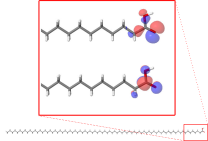
\includegraphics[scale=0.6]{Pics/NTOACID}
\caption[Dominant natural transition orbital pair for the lowest excitation of the carboxylic acid C$_{79}$H$_{159}$COOH.]{Dominant natural transition orbital pair for the lowest excitation of the carboxylic acid C$_{79}$H$_{159}$COOH ($\pi \rightarrow \pi^*$ transition). The span of the NTOs is very small compared to the rest of the molecule, and the compactness can be used to drastically speed up excited state calculations.}
\label{fig:NTO}
\end{figure}

\section{Atomic Orbital Configuration Interaction Singles}

%-> AO TDSCF (Kussmann)
%-> TDHF and RPA are equivalent in linear response regime. % see https://www.frontiersin.org/articles/10.3389/fphy.2019.00020/full

The methods presented in the previous section all work similarly. They first start by approximating the targeted excited states with a lower level of theory using CIS or CIS(D). They then solve higher order equations in the basis obtained from that approximation and may also dynamically augment the correlation domain while optimizing the excitation energies. The methods work on the principle of orbital \emph{compactness} rather than sparsity

At the moment of writing, CIS is the only excited state method which is routinely evaluated using an AO approach. While CIS does not give qualitatively good results, it is still a very important stepping stone for higher order methods, as was demonstrated in the previous section. Omitting the zero-order contributions, the CIS working equations are given by
\begin{equation}
r_{ia} = \left[ 2 \cn{ia}{jb} - \cn{ib}{ja} \right] u_{jb}
\end{equation}
\noindent Factoring out the MO coefficient matrices:
\begin{equation}
\begin{split}
r_{ia} &= C_{\mu i} C_{\sigma a} \left[ 2 \cn{\mu\sigma}{\nu\lambda} - \cn{\mu\lambda}{\nu\sigma} \right] C_{\nu j} C_{\lambda b} u_{jb} \\ 
&= C_{\mu i} C_{\sigma a} \left[ 2 \cn{\mu\sigma}{\nu\lambda} - \cn{\mu\lambda}{\nu\sigma} \right] P_{\nu\lambda} 
\end{split}
\end{equation} 
\noindent where $\mathbf{P}$ is the non-symmetric transition density in the AO basis. The CIS working equations can be reduced to the construction of a "pseudo"-Fock matrix which has a Coulomb and an exchange part. The Fock matrix is then transformed to the MO basis:
\begin{align}
F_{\mu\nu} &= J_{\mu\nu} + K_{\mu\nu}  \\ 
r_{ia} &= C_{\mu i} F_{\mu\nu} C_{\mu a}  
\end{align}
\noindent For localized excitations, the AO transition density is sparse (Figure \ref{fig:CISDENSE}), and similar approximation can be used as in Hartree Fock, e.g. LinK, CFMM, or LDF. CIS can therefore be evaluated with $\mathcal{O}(N)$ computational effort. Strictly speaking, it is not a "pure" AO formulation, because the AO intermediates still need to be transformed to the MO basis.

\begin{figure}
\centering
\begin{subfigure}{0.4\textwidth}
\centering
\includegraphics[width=\textwidth]{Pics/CISDENSE}
\caption{}
\end{subfigure}
$\Longrightarrow$
\begin{subfigure}{0.5\textwidth}
\centering
\includegraphics[width=\textwidth]{Pics/CIS}
\caption{}
\end{subfigure}
\caption[Logarithm of the absolute values of the matrix elements in the transition densities in the MO and AO basis for the lowest excited state for the carboxylic acid C$_{79}$H$_{159}$COOH.]{Logarithm of the absolute values of the matrix elements in the transition densities in the MO (left) and AO basis (right) for the lowest excited state for the carboxylic acid C$_{79}$H$_{159}$COOH. The excitation domain is entirely localized on the carboxylic group. Using sparse matrix algebra, significant speed-ups can be obtained for CIS in the AO basis.}
\label{fig:CISDENSE}
\end{figure}

% PAO CCLR not good! Look at Gunnar review article perhaps

% First appearance of local EOM-CCSD 
% Cra2002 https://aip.scitation.org/doi/pdf/10.1063/1.1537718

% First appearance of local CCLR CC2 (no doubles wrapping) Kat2006 https://aip.scitation.org/doi/pdf/10.1063/1.2339021
% Flaw: Domains dtermined from CCS, bad if not correponding to good approximat. ALso fixed during davidson

% Kat2009 https://aip.scitation.org/doi/pdf/10.1063/1.3237134
% FIxes Problem by refreshing domains

% state-specific PNOs from CIS(D) Hel2011 https://aip.scitation.org/doi/10.1063/1.3664902

% Hel2013 PNO-CC2 https://aip.scitation.org/doi/10.1063/1.4819071

% Hel2014 PNO-ADC2 https://www.sciencedirect.com/science/article/pii/S2210271X14001194?via%3Dihub

%PURE AO FORMULATION THOULESS INTEGRAL
%PROBLEM: MO ENERGIES ARE NEEDED. if a pure ao algorithm, most likely a whole other approach that tries to get "density metrix perturbation"

%\section{Molecular Orbital-free Approaches}

%Maybe if I have time
%https://aip.scitation.org/doi/full/10.1063/1.2961039?casa_token=XyapU_j1S9YAAAAA%3A6MKC3CuVoVEGS1bR-G3uHzyMo_UMcvArZKA2EkxO8Pwzc1gJWI0qwUWF6GB1PL7XEjDQH2lwrDniBQ
% https://aip.scitation.org/doi/10.1063/1.2965535

\chapter{The Spin-Opposite Scaled Algebraic Diagrammatic Construction Method in the Atomic Orbital Basis}

The Algebraic Diagrammatic Construction method can be considered as M{\o}ller Plesset for excited states. It is therefore not surprising that local correlation method for MP can also be applied to MP. In chapter ..., it has been shown that local approximations for the ground state can be grouped into 3 categories: atomic orbitals, local orbitals and natural orbitals. Only the latter two have been used in the context of ADC as discussed in chapter .... An atomic orbital representation of ADC has not yet been considered in literature, and will be the subject of this chapter. First, the restricted doubles-folded ADC working equations are derived. Then the SOS approximation is applied. Finally, the restricted SOS-ADC working equations are derived in the AO basis, with and without density fitting. 

\section{Working Equations for Restricted ADC with Doubles-Folding}

The eigenvalue problem in the algebraic diagrammatic construction method truncated at doubles excitations takes the form
\begin{equation}
\begin{bmatrix}
\mathbf{A}_{SS} & \mathbf{A}_{SD} \\
\mathbf{A}_{DS} & \mathbf{A}_{DD}
\end{bmatrix} =  
\begin{bmatrix}
\mathbf{v}_{S} \\
\mathbf{v}_{D}
\end{bmatrix}
\mathbf{\Omega}
\end{equation}
\noindent where $\mathbf{A}$ is the symmetric Jacobian ADC matrix with the singles-singles (SS), doubles-singles (DS), singles-doubles (SD) and doubles-doubles (DD) sub-blocks, with the eigenvectors $\mathbf{v}$ and the diagonal eigenvalue matrix $\Omega$. The eigenvalue problem in Equation ... is generally solved using the Davidson diagonalization procedure (A2) to extract the first few lowest eigenvalues. Rather than constructing the entire Jacobian matrix which scales as $\ccpx{8}$ using Equations ... to ..., the Davidson method computes the matrix-vector products $\mathbf{r} = \mathbf{A} \mathbf{u}$ with the current trial vectors $\mathbf{u}$ using a closed-form expression, which reduces the computational complexity to $\ccpx{5}$. The MVPs can be expressed in block-form as
\begin{equation}
\begin{split}
\mathbf{r}_{S} = \mathbf{A}_{SS} \mathbf{u}_{S} + \mathbf{A}_{SD} \mathbf{u}_{D} \\
\mathbf{r}_{D} = \mathbf{A}_{DS} \mathbf{u}_{S} + \mathbf{A}_{DD} \mathbf{u}_{D}
\end{split} 
\end{equation}
\noindent The trial vector space in the Davidson diagonalization scales with fourth order as $o^2v^2$, and can quickly become a memory bottle-neck for large molecules. As shown in the previous chapter, one can recompute the doubles-part of the MVP on-the-fly using \emph{doubles-folding}
\begin{equation}
\mathbf{r}_S(\omega) = \mathbf{A}_{SS} \mathbf{u}_{S} + \frac{\mathbf{A}_{SD}}{\omega - \mathbf{DD}} \mathbf{u}_{S} 
\end{equation} 
\noindent This trick is only possible for ADC(2)-s where the doubles-doubles block of the ADC matrix is diagonal. While the memory footprint for the diagonalization is reduced from $o^2v^2$ to $ov$, the MVP becomes dependent on the eigenvalue $\omega$ and a modified Davidson procedure needs to be used to solve this \emph{pseudo}-eigenvalue value (A...). 

The above expression is valid in the case of unrestriced ADC(2) where molecular \emph{spin}-orbitals are assumed, rather than \emph{spatial} orbitals. The working equations for standard ADC(2) and doubles-folded ADC(2) are given in Table ... . Implementations such as adcman in Q-Chem can use these formulae directly by delegating any considerations of spin-symmetry to a special tensor library called libtensor, which programmatically keeps track of the non-vanishing spin block components and reduces the expressions to the restricted ADC(2) equations for closed-shell molecules (Figure ...).

If no special block tensor library is used, it is numerically advantageous to split the ADC(2) matrix-vector products into their spin-components, and compute each block individually. Using a double-bar notation to indicate MOs with opposite spin $\sigma(i) \neq \sigma(\ool{i})$, the matrix-vector product can be written as
\begin{equation}
\begin{split}
r_{ia}( \omega) = &(\eps_a - \eps_i) u_{ia} - \sum_{jb} \left[ \cn{ij}{ab} - \cn{ia}{jb} \right] u_{jb} + \sum_{\ool{jb}} \cn{ia}{\ool{jb}} u_{\ool{jb}} \\
&+ \sum_b I_{ab} u_{ib} + \sum_{j} I_{ij} u_{ja} - \frac{1}{2} \left[ t_{ia\ool{jb}} I^{(1)}_{\ool{jb}} + \cn{ia}{\ool{jb}} I_{\ool{jb}}^{(2)} \right] \\
&- \frac{1}{2} \left[ \left( t_{iajb} - t_{jaib} \right) I^(1)_{jb} + \left(\cn{ia}{jb} - \cn{ja}{ib} \right) I_{jb}^{(2)} \right] \\
&+ \sum_{kcl} u_{kalc}(\omega) \cn{ik}{cl} + \sum_{k\ool{cl}} u_{ka\ool{lc}}(\omega) \cn{ik}{\ool{cl}} \\
&- \sum_{ckd} \cn{ac}{kd} u_{ikcd}(\omega) - \sum_{c\ool{kd}} \cn{ac}{\ool{kd}} u_{ic\ool{kd}}(\omega)
\end{split}
\end{equation}  
\noindent with the pre-iteration intermediates (computed only once)
\begin{equation}
\begin{split}
I_{ab} &= \frac{1}{2} \sum_{kcl} \left[ t_{kalc} \cn{kb}{lc} - t_{kalc} \cn{kc}{lb} + \cn{ak}{cl} t_{kblc} - \cn{al}{ck} t_{kb}{lc} \right] \\
&+ \frac{1}{2} \sum_{k\ool{cl}} \left[ t_{ka\ool{lc}} \cn{kb}{\ool{lc}} + \cn{ak}{\ool{cl}} t_{kb}{\ool{lc}} \right] 
\end{split}
\end{equation}
\begin{equation}
\begin{split}
I_{ij} &= \frac{1}{2} \sum_{ckd} \left[ t_{ickd} \cn{jc}{kd} - t_{ickd} \cn{jd}{kc} + \cn{ci}{dk} t_{jckd} - \cn{ck}{di} t_{jckd} \right] \\
&+ \frac{1}{2} \sum_{c\ool{kd}} \left[ t_{ic\ool{kd}} \cn{jc}{\ool{kd}} + \cn{ci}{\ool{dk}} t_{jc\ool{kd}} \right]  
\end{split}
\end{equation}
\noindent and the iteration intermediates which depend on the trial vectors $\mathbf{u}$ (computed at each Davidson iteration)
\begin{equation}
I_{ia}^{(1)} = \sum_{jb} \left[ \cn{ja}{ia} - \cn{ja}{ib} \right] u_{jb} + \sum_{\ool{jb}} \cn{\ool{jb}}{ia} u_{jb}
\end{equation}
\begin{equation}
I_{ia}^{(2)} = \sum_{jb} \left[ t_{iajb} - t_{jaib} \right] u_{jb} + \sum_{\ool{jb}} t_{ia\ool{jb}} u_{\ool{jb}}
\end{equation}
\noindent The doubles components are computed on-the-fly and read
\begin{equation}
\begin{split}
u_{iajb}(\omega) &= \frac{1}{\omega - \eps_a - \eps_b + \eps_i + \eps_j} \left\lbrace \sum_k \left[ u_{ka} \cn{ki}{bj} - u_{ka} \cn{kj}{bi} - u_{kb} \cn{ki}{aj} \right. \right. \\
&+ \left. \left. u_{kb} \cn{kj}{ai} \right] - \sum_c \left[ u_{ic} \cn{ac}{bj} - u_{ic} \cn{aj}{bc} - u_{jc} \cn{ac}{bi} + u_{jc} \cn{bc}{ai} \right] \right\rbrace
\end{split}
\end{equation}
\begin{equation}
\begin{split}
u_{ia\ool{jb}}(\omega) = \frac{1}{\omega - \eps_a - \eps_b + \eps_i + \eps_j} \left\lbrace \sum_k u_{ka} \cn{ki}{\ool{bj}} + \sum_{\ool{k}} u_{\ool{kb}} \cn{\ool{kj}}{ai} \right. \\ - \sum_c u_ic \cn{ac}{\ool{bj}} - \left. \sum_{\ool{c}} u_{\ool{jc}} \cn{\ool{bc}}{ai} \right\rbrace
\end{split}
\end{equation}
\noindent The expression for the MVP for beta electrons ($r_{\ool{ia}})$ is obtained by replacing alpha orbitals ($i$) by beta orbitals ($\ool{i}$) and vice-versa in the expressions above. The off-diagonal blocks $r_{i\oola}$, i.e. the spins-flip states will not be considered here and are set to zero. For closed-shell molecules, the complexity of the formulas can be drastically reduced by introducing the following spin-symmetry relationships:
\begin{equation}
\begin{split}
t_{iajb} = t_{ia\ool{jb}} = t_{\ool{ia}jb} = t_{\ool{iajb}} \\
\cn{ia}{jb} = \cn{ia}{\ool{jb}} = \cn{\ool{ia}}{jb} = \cn{\ool{ia}}{\ool{jb}} 
\end{split}
\end{equation}
\begin{equation}
\begin{split}
u_{ia} &= u_{\ool{ia}} \qquad \textrm{if singlet} \\
u_{ia} &= - u_{\ool{ia}} \qquad \textrm{if triplet} 
\end{split}
\end{equation}
\noindent One then obtains two separate expressions for restricted ADC(2), depending on whether singlet or triplet states are addressed
\begin{equation}
\begin{split}
r_{ia}^S(\omega) &= (\eps_a - \eps_i) u_{ia} - \sum_{jb} \left[ 2\cn{ij}{ab} - \cn{ia}{jb} \right] u_{jb}^S + \sum_b I_{ab} u_{ib} + \sum_j u_{ja}^S I_{ij} \\
&- \frac{1}{2} \sum_{jb} \left[2t_{iajb} - t_{ibja}\right] I^{(1)S}_{jb} - \frac{1}{2} sum_{jb} \left[ 2 \cn{ia}{jb} - \cn{ib}{ja} \right] I^{(2)S}_{jb} \\
&+ \sum_{kcl} \cn{ik}{lc} \left( 2 u_{kalc}^S(\omega) - u_{lakc}^S(\omega) \right) + \sum_{ckd} \left( 2 u^S_{ickd}(\omega) - u^S_{kcid}(\omega) \right) \cn{kd}{ac}  
\end{split}
\end{equation} 
\begin{equation}
\begin{split}
r_{ia}^T(\omega) &= (\eps_a - \eps_i) u_{ia}^T - \sum_{jb} \cn{ij}{ab} u_{jb}^T + \sum_b I_{ab} u_{ib}^T + \sum_j I_{ij} u_{ja}^T \\
&+ \frac{1}{2} \sum_{jb} t_{ibja} I^{(1)T}_{jb} + \frac{1}{2} \sum_{jb} \cn{ib}{ja} I^{(2)T}_{jb} \\
+& \sum_{kcl} \cn{ik}{lc} \left[ 2 u^T_{kalc}(\omega) - u^T_{lakc}(\omega) - u^T_{kcla}(\omega) \right] \\
+& \sum_{ckd} \left[ 2 u^T_{ickd}(\omega) - u^T_{idkc}(\omega) - u^T_{kcid}(\omega) \right] 
\end{split}
\end{equation}
\noindent with the singlet and triplet doubles intermediates
\begin{equation}
\begin{split}
u^S_{iajb}(\omega) = \frac{1}{\omega - \eps_a + \eps_i - \eps_b + \eps_j} \left\lbrace \sum_k \left[ u^S_{ka} \cn{ki}{jb} + u^S_{kb} \cn{kj}{ai} \right] \right. \\
\left. - \sum_c \left[ u^S_{ic} \cn{jb}{ac} - u^S_{jc} \cn{ib}{ac} \right] \right\rbrace
\end{split} 
\end{equation}
\begin{equation}
u^T_{iajb}(\omega) = \frac{1}{\omega - \eps_a + \eps_i - \eps_b + \eps_j} \left\lbrace \sum_k u^T_{ka} \cn{ki}{bj} - \sum_c u^T_{ic} \cn{ac}{jb} \right\rbrace
\end{equation}
\noindent The pre-iteration intermediates are given by
\begin{equation}
I_{ab} = \frac{1}{2} \sum_{kcl} \left[ \left( 2t_{kalc} - t_{kcla}\right) \cn{kb}{lc} + \left( 2t_{kblc} - t_{kclb} \right) \cn{ka}{lc} \right]
\end{equation}
\begin{equation}
I_{ij} = \frac{1}{2} \sum_{ckd} \left[ \left( 2t_{ickd} - t_{idkc}\right) \cn{jc}{kd} + \left( 2t_{jckd} - t_{jdkc} \right) \cn{ic}{kd} \right]
\end{equation}
\noindent and are the same for both singlet and triplet expressions. The iterative intermediates however are split:
\begin{equation}
I^{(1)S}_{ia} = \sum_{jb} \left( 2\cn{ia}{jb} - \cn{ib}{ja} \right) u_{jb}^S
\end{equation}
\begin{equation}
I^{(2)S}_{ia} = \sum_{jb} \left( 2t_{iajb} - t_{ibja}\right) u_{jb}^S
\end{equation}
\begin{equation}
I^{(1)T}_{ia} = - \sum_{jb} \cn{ib}{ja} u_{jb}^T
\end{equation}
\begin{equation}
I^{(2)T}_{ia} = - \sum_{jb} t_{ibja} u_{jb}^T
\end{equation}
\noindent For the restricted equations ... to ..., the indices $ijkl...$ and $abcd...$  represent the occupied and virtual spin-integrated \emph{spatial} molecular orbitals. 

\section{Working Equations for Restricted SOS-ADC with Doubles-Folding}

In the restricted ADC expressions for the matrix-vector product, the 4-index intermediates $u_{iajb}(\omega)$ need to be evaluated and temporarily stored, even if the density fitting approximation is used. This memory-intensive step can be avoided by using spin-opposite scaling (Section ...). Consider again the approximations introduced by the SOS method for the unrestricted ADC(2) matrix equations
\begin{itemize}
\item In the spin-amplitudes $\hat{t}_{iajb}$ the same-spin contributions are nulled and the opposite-spin contributions are scales by $c_os$
\begin{equation}
\hat{t}_{SOS} = c_{os} \hat{t}_{iajb} \left( 1 - \delta_{\sigma (i) \sigma (j)} \right)
\end{equation}
\item In the doubles-singles and singles-doubles block of the ADC matrix, some same-spin contributions are also removed, and the whole block is scaled by a different constant $c_{osc}$ 
\begin{equation}
C_{ia,kcld} = c_{osc} \left[ \sbk{kl}{id} \delta_{ac} - \sbk{kl}{ic} \delta_{ac} - \sbk{al}{cd} \delta_{ik} + \sbk{ak}{cd}\delta_{il} \right] \left( 1 - \delta_{\sigma (k) \sigma (l)} \right)
\end{equation}
\begin{equation}
C_{iajb,kc} = c_{osc} \left[ \sbk{kb}{ij} \delta_{ac} - \sbk{ka}{ij} \delta_{bc} - \sbk{ab}{cj} \delta_{ik} + \sbk{ab}{ci}\delta_{jk} \right] \left( 1 - \delta_{\sigma (i) \sigma (j)} \right)
\end{equation}
\noindent Here, the function $\sigma(x)$ returns the spin of orbital $x$.
\end{itemize}

%\noindent If singlet:
%\begin{equation}
%\begin{split}
%u_{ia} = u_{\ool{ia}} := v^S_{ia} \\
%u_{iajb} = u_{\ool{iajb}} := v^S_{iajb} - v^S_{ibja} \\
%u_{ia\ool{jb}} := u^{S}_{iajb}
%\end{split}
%\end{equation}
%\noindent If triplet 
%\begin{equation}
%\begin{split}
%u_{ia} = - u_{\ool{ia}} := v^T_{ia} \\
%u_{iajb} = - u_{\ool{iajb}} := v^T_{iajb} - v^T_{ibja} - v^T_{jaib} + v^T_{jbia} \\
%u_{ia\ool{jb}} := u^{T}_{iajb} - u^T_{jbia}
%\end{split}
%\end{equation}

\chapter{Benchmarking and Results}

\section{Ground-State}

\section{Excited-State}

\part{}

\chapter{Parallel Computing}

The popularity of computational chemistry can be attributed in no small part to the advances and devlopment of highly efficient algorithms in theoretical chemistry. Equally important however is the ever increasing accessibility and performance of computing resources: commercially available work stations can handle chemical systems which could only be modelled on supercomputers a couple decades ago, and firmly cemented the position of computational chemsitry as an important "experimental" tool in the toolbox of a chemist. 

As the speed of computers increased over the years, so did the complexity of their components. Nowadays, programmers can choose between several types of architectures, such as shared or distributed memory systems, or accelerators like GPUs. Knowing the strenths and weaknesses of each type is paramount to developing efficient algorithms and tackling larger molecular systems.

This chapter gives an overview on computer architecture, and the different types of parallelism encountered on modern hardware.

\section{Moore's Law}

\emph{Moore's Law} states that the transistor density in integrated chips doubles every 12 to 24 months. First formulated in 1965 by Gordon More, his prediction has held up fairly well over the years. However, the technology enabling this trend has changed over the years.

Figure ... shows the trends in clock speed, single-thread performance, power consumption and number of logical cores and transistors for microprocessors from 1970 to 2000. Since the early 2000s, clock-speed and single-thread performance have begun to plateau, and have stagnated from 2010 onwards. Increasing the clock speed to values beyond 4 to 5 GHz generates too much stress on the microchip in form of heat, and decreases its performance. This flaw was compensated by using the growing transistor density to instead increase the number of logical cores on a single chip. 

Shifting towards increasing core count however entails that the most ideal perfpormance of a CPU can only be achieved though parallel programming. With the rise of parallel computing, the number of different parallel hardware features drastically increased, and it can be difficult for programmers to fully exploit the available computing resources. Moreover, different programming language and compiler extensions have emerged alongside, with numerous competing standards, especially for GPUs. 

\begin{figure}
\centering
\includegraphics[scale=1.2]{Pics/moore}
\caption{Taken from \protect\url{https://github.com/karlrupp/microprocessor-trend-data}}
\end{figure}

\section{Benefits and Limits of Parallel Computing}

While the different available programming models can seem daunting at first, one of the major advantages of parallel computing is improved \emph{scalabilty}. An application that exposes parallelism can be sped up by several orders of magnitude, simply by adding more compute power, with several different architectures to choose from. The limit of what problem sizes can be tackled is mostly dictated by the \emph{amount} of available computing resources and storage, rather than individual processor charcterstics.

As important as parallel computing has become in recent years, there is a reason why increasing clock speed was seen as the foremost strategy in keeping Moore's law alive. First, modifying a serial program to exploit parallelism can be a time-consuming endeavour, and second, not all tasks can be effectively parallelized. This means that the potential amount of seed-up is limited by the amount of parallel code. This is known as \emph{Amdahl's law}. The speed-up for a number of cores $N_c$ is given by
\begin{equation}
Speed-Up(N_c) = \frac{1}{S + \frac{P}{N_c}}
\end{equation}
\noindent where $S$ is the fraction of serial code and $P$ is the fraction of parallel code. The speedup for a fixed-size problem as a number of cores is known as \emph{strong scaling}, and the time-to-solution on each indivual core \emph{decreases} when more cores are added.

An alternate way to compute potential speed-up is given by Gustafson-Barsis's Law
\begin{equation}
Speed-Up(N_c) = N_c - S(N_c-1)
\end{equation}
\noindent where the problem size also increases proportionally to the number of cores. The scaling for this trend is known as \emph{weak scaling}. In this scenario, the time-to-solution spend on each core remains constant, as the system size and number of cores increases. Even if this type is called "weak", both forms of scaling are equally important, as they adress different scenarios. 

\section{Types of Parallelism and Memory Hierarchy}

Nowadays, a programmer has access to four categories of parallelism:
\begin{enumerate}
\item vectorization
\item thread-based parallelism
\item process-based parallelism
\item streaming
\end{enumerate} 
\noindent Leveraging the power of each type requires some understanding of the underlying hardware. 

Figure \ref{clusterArchitecture} shows the major components and memory pathways in a modern computing cluster. A \emph{cluster} is a collection of individual computers that work together and form a single unit. Individual computers are also called \emph{nodes} and occupy a single rack (or "shelf") each in a large server cabinet. The nodes are connected via a low-latency, high through-put network, e.g. ethernet cables to enable inter-node communication. Each node contains one or more central proecessing units (CPU) and optionally one or more graphical processing units (GPU). Systems where different types of hardware architecture are mixed are also known as \emph{heterogenous} systems. The individual components are fixed on a \emph{motherboard}: CPUs are plugged into \emph{sockets} and GPUs into \emph{PCIe slots}. A CPU is composed of one or more cores, where the actual processing of data is carried out. A GPU is also composed of multiple cores, which are grouped into independent \emph{streaming multiprocessors} (SM). 

\begin{figure}
\centering
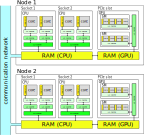
\includegraphics[scale=1.0]{Pics/memory}
\caption{Memory hierarchy}
\label{clusterArchitecture}
\end{figure}

Memory is also a crucial component of computer architecture and is a limited resource. The speed at which data is read from memory can also become a major bottle-neck: No matter how fast a processor is, if the feed rate is too low, it cannot reach its peak performance becuase it wastes cycles while waiting for data to arrive. To optimize data through-put, the memory model in modern computer architecture requires a complex hierarchy, with different sizes and speeds. Computer memory at the top of the hierarchy has a high response rate, but low complexity. It is also very expensive to produce and therefore much smaller. At the bottom of the hierarchy is memory with large storage space and capable of complex tasks. It is cheap but has low reponse rate. Over the years, the number of levels in the memory hierarchy has increased. Most modern computers have six levels: CPU registers, L1 chache, L2 chache, L3 chache, DRAM and disk. 

CPU registers sit at the top of the hierarchy and are closest to the cores. It is the region of memory where data is directly manipulated by arithmetic operations and machine code. Its size is typically on the order of several tens to hundreds of bytes. Data is loaded into the registers from \emph{cache}, a region of memory which is further subdivided into different levels named L1, L2 and L3. Each core has its own L1 cache, but might share L2 and L3 cache with other cores. Caches have different sizes and speeds, with L1 being the fastest and smallest at several tens of kB, and L3 being the slowest and largest at several tens to hundreds of kB. Memory is transferred from L3, to L2, to L1 and finally to the CPU registry. The reason why there are multiple levels of chache is to reduce \emph{cache misses}. If data requested by the core is not found in L1, then L2 is searched, then L3. A cache miss is an event where the data is not found anywhere in chache. In that case, a request has to be put out to the dynamical random access memory (DRAM) to retrive data. Modern techniques such as \emph{chache prefetching} can minimize the amount of cache misses by loading the data into higher chache levels before it is actually needed by the lower levels. 

The speed of DRAM is 10 to 100 time slower than cache, but much larger in size. It is the main memory pool and shared by all cores. CPUs and GPUs have separate DRAM regions which communicate via a PCIe bus. DRAM sizes vary drastically, and are on the order of 10$^0$ to 10$^1$ for GPUs and 10$^0$ to 10$^3$ for CPUs. Data can be transferred from one node to another via CPU DRAM through the communication network, with transfer rates on the order of several GB/s. For programs which are not reading from disk, this is weakest link in the memory hierarchy ???

\section{Vectorization}

Vectorization is the pocess of operating on multiple variables at the same type. This type of parallelism is encountered at the highest level of the memory hierarchy introduced in the previous section, i.e. CPU registers. Each core has multiple registers, also called \emph{vector registers} with a certain size or \emph{vector length}. Instead of loading each inidividual element from cache and operating on it, one vector operation on a range of elements can replace multiple single operations. For a 512-bit register, two vectors with 8 floats (32 bit) can be summed within one cycle instead of eight (Figure ...). This type of parallelism is also known as single instruction multiple data (SIMD). 

The length of vector registers, number of registers as well as the number of supported vector operations have greatly expanded over the years (Table \ref{VECTORHARDWARE}).

\begin{table}
\makegapedcells
\centering
\begin{tabular}{p{0.3\linewidth}cc}
\hline
Release & Vector Length (bit) & No. Registers \\ \hline
SSE (Streaming SIMD Extension) & 128 & 8 \\ 
SSE2/SSE3/SSE4 & 128 & 16  \\
AVX/AVX2 (advanced vector instructions) & 256 & 16 \\
AVX512 & 512 & 32 \\ 
\hline 
\end{tabular}
\caption{Adpated from ...}
\label{VECTORHARDWARE}
\end{table}

\subsection{Parallel SAXPY using vectorization}

To show how vectorization can be introduced into a program, consider the following vector operation:
\begin{equation}
y \leftarrow \alpha x + y
\label{DAXPY}
\end{equation}
\noindent where $y$, $x$ are vectors of equal length, and $\alpha$ is a scaling factor. The vector operation \ref{DAXPY} is also known as "saxpy" for single precision, and "daxpy" for double precision. A naive implementation of the saxpy-kernel is given in Listing \ref{lst:SAXPYNOPARA} for vector size $N$  

\cppcode{Parallelization-unaware implementation of saxpy \label{lst:SAXPYNOPARA}}{saxpy_nopara.c}

\noindent Two arrays are allocated, x and y, and all their entries set to 1 and 2 respectively. Each element is updated individually in the for loop. There are several possibilities to introduce vectorization:
\begin{enumerate}
\item auto-vectorization
\item compiler directives
\item intrinsic functions
\item optimized libraries
\end{enumerate}
\noindent Auto-vectorization is by far the easiest approach: the compiler automatically recognizes that the loop can be vectorized and generates optimized machine code that uses vector instructions. This does not require any input from the user. Compiling the code on a machine with AVX support, using the GNU C compiler, and passing the compiler flags "-O2 -march=native -ftree-vectorize -fopt-info-vec-optimized" generates the following report:
\begin{lstlisting}[backgroundcolor=\color{light-gray},breaklines=true]
saxpy_nopara.c:9:3: optimized: loop vectorized using 32 byte vectors
\end{lstlisting}
\noindent which indicates that the vectors are loaded and operated on in 32 byte chunks, or 8 floats at once. The flag "-ftree-vectorize" (or alternatively "-O3") activates auto-vectorization and "-fopt-info-vec" generates the report. To make sure that the C compiler uses the right vectorization relase, the flag "-march=native" is needed, or else the comiler might fall back to SSE. 

In some cases, auto-vectorization cannot take place because the compiler did not recognize that the loop can be vectorized. It can then be beneficial to use \emph{intrinsic functions}. Intrinsic functions are compiler-dependent functions that map to processor operations. When targeting an AVX architecture with 256-bit registers, the saxpy kernel can be rewritten as
\cppcode{SAXPY using intrinsics \label{lst:SAXPYINTRINSICS}}{saxpy_intrinsic.c}
\noindent It is apparent that using intrinsics makes the program much more complex. The arrays cannot be fed directly to the functions, but need to be loaded into vectors of type \texttt{\_\_mm256}, using "set" or "load" functions. Furthermore, the data needs to be aligned correctly using \texttt{\_\_attribute\_\_ ((aligned(...)))}. The arrays are then loaded in chunks into the registers and given to the vector functions for multiplying and adding. 

The major problem with using intrinsic functions, besides increased complexity, is \emph{portability}. The code in \ref{lst:SAXPYINTRINSICS} does not compile on machines that do not support AVX, and is limited to 256-bit registers even on AVX-512 machines. Portable alternatives include using compiler directives or optimized libraries.

Directives (or "pragmas") are hints that can be given to the compiler that suggest that the loop might be vectorizeable. By far the most popular set of compiler directives that provide vectorization capabilities is undoubtedly included in the OpenMP application programming interface (API). The OpenMP API is standardized accross all compilers, making it highly portable. The OpenMP directives greatly simplify the SAXPY program:
\cppcode{SAXPY using compiler directives \label{lst:SAXPYDIRECTIVES}}{saxpy_openmp.c}
\noindent Simply plopping the directive in front of the for loop takes care of generating the appropriate machine code for the targeted architecture. 

The last way to introduce vectorization is via external programs, such as the basic linear algebra subprograms (BLAS) library. It provides a set of specific functions for performing basic vector and matrix operations. Similar to OpenMP, it only provides spcifications, and the direct implementation is compiler-dependent. In the BLAS routines, there is a saxpy functions available that can be called directly. It has the advantage of completely removing the loop and clearly states what operation is performed.
\cppcode{SAXPY using BLAS \label{lst:SAXPYBLAS}}{saxpy_blas.c}
\noindent External libraries can however be associated with a steeper learning curve depending on the complexity of function signatures.

\section{Thread-based Parallelism}

\section{Process-based Parallelism}

\section{Steaming}

Why parallel computing?
-> becomes increasingly important, programmers should be well versed in it

Moores's Law

Fundamental law's: Amdahl

Types of parallelism:
- vectorization
- threads
- processes
- streaming (GPU)

Work at different levels of hardware

SETI@HOME

Categorizing parallel approaches Flynn's Taxonomy

errors in parallelism (p.40-41)

Performance limits
Levels of memory : speed vs feed (p. 59) show example of sizes of L caches



\chapter{Into The Matrix}

At its core, computational chemistry is basically matrix algebra applied to molecular systems. The performance of an algorithm, in other words its scaling, memory footprint and even accuracy, is intimately linked to how matrix operations and storage are handled internally. While the earliest implementations of molecular electronic structure methods often used hand-coded loops running over matrix indices, over the years, a whole ecosystem of matrix and tensor libraries has emerged in an attempt to lessen the burden of programmers, to various degrees of success, each with their strong and weak points. Choosing the best library for an algorithm is a non-trivial task, and depends on various factors: if memory is the bottle-neck, a sparse matrix library might be able to sufficiently compress data into a smaller space. If speed is the greatest concern, targeting different architectures like distributed memory systems, accelerators, or both, might be the solution.

This chapter introduces basic concepts of matrix and tensor algebra, with a focus on storage orders. After introducing the core concepts, a small list of matrix libraries used in \mchem{} is provided which summarizes the core functionalities.´

\section{Linear Algebra}

Linear algebra is a crucial tool in many areas of computational science, such as image processing, machine learning, computational physics, computational biology and of course computational chemistry. The most important concepts are discussed in this section. Until mentioned otherwise, zero-based indexing is assumed. 

\subsection{Matrices}

A matrix is a rectangular, 2-dimensional array of dimension $M$ by $N$, containing a set of complex or real numbers $\{a_{ij}\}$ with ordered subscripts $i = 0,1,2,...M$ and $j = 0,1,2,...,N$, of the form
\begin{equation}
\mbf{A} = \begin{pmatrix}
a_{00} & a_{01} & \ldots & a_{0N} \\
a_{10} & a_{11} & \ldots & a_{1N} \\
\vdots & \vdots & \ddots & \vdots \\
a_{M0} & a_{M1} & \ldots & a_{MN}
\end{pmatrix}
\end{equation}
\noindent with $M$ \emph{rows} and $N$ \emph{columns}. \emph{Row vectors} and \emph{column vectors} are types of matrices that contain only one row or one column, respectively. 

Matrix multiplication is only defined between matrices of dimension $M$ by $K$ and $K$ by $N$. The product yields an $M$ by $N$ matrix
\begin{align}
\mbf{C}_{M\times N} &= \mbf{A}_{M\times K} \mbf{B}_{K\times N} \\
c_{ij} &= \sum_k a_{ik} b_{kj}
\end{align}

A matrix with an equal number of rows and columns is called a \emph{square matrix}. There a different types of square matrices:
\begin{enumerate}
\item \emph{Diagonal matrices} only have non-zero entries on the diagonal
\begin{equation}
a_{ij} = a_{ii} \delta_{ij}
\end{equation}

\item If all entries below the diagonal are zero, the matrix is \emph{lower triangular}. Similarly, if all elements above the diagonal are zero, the matrix is \emph{upper triangular}. Furthermore, if the diagonal entries are all equal to 1, the matrix is \emph{unit triangular}.

\item The \emph{identity} or \emph{unit} matrix $\mbf{1}$ is defined as
\begin{align}
\mbf{A} \mbf{1} &= \mbf{1} \mbf{A} \\
\mbf{1}_{ij} &= \delta_{ij}
\end{align} 

\item The \emph{inverse} of a matrix $\mbf{A}$ is defined as
\begin{equation}
\mbf{A}^{-1} \mbf{A} = \mbf{1}
\end{equation} 
\noindent It only exists for matrices with a non-zero determinant. If a matrix is non-invertible, it is also called \emph{singular}. 

\item A matrix is \emph{unitary}, if its inverse is equal to its conjugate transpose 
\begin{equation}
\mbf{A}^{-1} = \mbf{A}\pdg
\end{equation}
\noindent A real unitary matrix is called \emph{orthogonal}

\item A \emph{hermitian} matrix is its own conjugate transpose
\begin{align}
\mbf{A} &= \mbf{A}\pdg \\
a_{ij} &= (a_{ji})^*
\end{align}
\noindent A real hermitian matrix is called \emph{symmetric}

\item A hermitian matrix is said to be \emph{positive definite} if all of its eigenvalues are positive, and \emph{negative definite} if all eigenvalues are negative. \emph{Semi-definite} matrices additionally have some eigenvalues which are equal to zero.   
\end{enumerate}

%\subsection{Matrix Decompositions}
%
%Matrix decomposition (or factorization) is one of the fundamental disciplines in linear algebra. Decompositions reduce a matrix into a product of matrices. They can be used to solve a system of linear equations, solve the linear least squares problem, invert a matrix, analyze the numerical stability of a system, or find the \emph{rank} of a matrix, i.e. the number of linearly independent column vectors. Some decomposition techniques can factorize a large and complex matrix into smaller constituents that are more easy to operate on. Examples of matrix decomposition algorithms include
%\begin{enumerate}
%
%\item The \emph{eigenvalue decomposition} finds a transformation matrix $\mbf{V}$ such that it diagonalizes the matrix
%\begin{equation}
%\mbf{A} = \mbf{V} \boldsymbol{\Lambda} \mbf{V}^{-1}
%\end{equation}
%\noindent where $\boldsymbol{\Lambda}$ is a diagonal matrix containing the eigenvalues. This decomposition is only possible for square matrices.
%
%\item The \emph{LU} factorizes a symmetric matrix into a product of a lower triangular matrix $\mbf{L}$ with its transpose
%
%\end{enumerate}

\section{Matrix Storage Formats}

The main memory in a computer, i.e. DRAM, is a linear address space and can be seen as a single, contiguous, one-dimensional array. Two-dimensional arrays like matrices need to be \emph{mapped} to this linear space by the compiler. This mapping depends on whether a dense or sparse view of the matrix is desired. 

\subsection{Dense Storage}

There are two ways to map a dense matrix to memory: row-major ordering and column-major ordering. The two storage orders differ by the order in which the individual elements are stored in memory. For an $M$ by $N$ matrix stored in a linear array $a$ in row-major format, the address offset of an element $a_{ij}$ compared to element $a_{00}$ is given by
\begin{equation}
A(i,j) \rightarrow \text{a[i * N + j]}
\end{equation}
\noindent and in column-major format by
\begin{equation}
A(i,j) \rightarrow \text{a[i + j * M]}
\end{equation}
Neither storage order has any advantages or disadvantages over the other one. It is only a matter of convention, and depends on the library and programming language. Fortran arrays are column-major, while C/C++ arrays are row-major. 

However, algorithms optimized for column-major access might not give the same performance for row-major formats and vice-versa. Consider a simple loop over matrix elements in the Fortran programming language
\begin{fortran}{Matrix Loop \label{FORTRAN1}}
DO i = 1, N
 DO j = 1, N
  A(i,j) = A(i,j) + 2
 ENDDO
ENDDO
\end{fortran}
\noindent By first looping over the rows, and then over the columns, the elements in the column-major matrix are accessed in a \emph{non-contiguous} manner. This prevents efficient optimizations like vectorization due to cache misses. By swapping the loops, the inner loop can be vectorized. Therefore, if algorithms assume a certain ordering, it is important to pass matrices of the same ordering.

Column-major ordering is by far the most common in scientific computing. Matrix algebra routines like the QR, Eigenvalue or Cholesky decompositions are most intuitively written using column operations rather than row operations. Examples include the LAPACK and Eigen matrix libraries. 

\subsection{Sparse Storage}

A matrix is called \emph{sparse} if "most" of its elements are zero. The threshold between sparse and dense is ill-defined, and range anywhere between 1\% and 10\%. Sparse matrices are encountered in many fields of computational science in systems with few pair-wise interactions. By storing and looping over the significant elements only, the memory footprint and the scaling of matrix multiplications or decompositions can be significantly reduced. There are several different sparse matrix formats available. The following sections will demonstrate how the matrix
\begin{equation*}
\begin{pmatrix}
3 & 5 & 0 & 0 \\
0 & 4 & 0 & 0 \\
0 & 0 & 1 & 2 \\
0 & 0 & 6 & 7 
\end{pmatrix}
\end{equation*}
\noindent may be represented using some of these formats.

\subsubsection{Coordinate Format}

The coordinate format (COO) is one of the simplest storage schemes for sparse matrices. The matrix is stored using three arrays of length $NNZ$ (number of non-zero elements) containing the row indices, column indices and matrix entries. The above matrix reduces to 
\begin{equation*}
COO: \left\lbrace
\begin{matrix}
\textrm{idx\_i} &= &\left[ 0, 0, 1, 2, 3, 2, 3 \right] \\
\textrm{idx\_j} &= &\left[ 0, 1, 1, 2, 2, 3, 3 \right] \\
\textrm{val}   &= &\left[ 3, 5, 4, 1, 6, 2, 7 \right] \\
\end{matrix}
\right.
\end{equation*}
\noindent The values do not need to be necessarily ordered. The COO format has the advantage that it is very easy to insert elements and change the sparsity pattern with low overhead. COO is generally not used for algebra due to slow random access of elements if they are not stored in order. Rather, COO is an intermediate format for incremental construction of sparse matrices in the CSR or CSC format.

\subsubsection{Compressed Sparse Row}

The compressed sparse row format (CSR) is similar to COO, but compresses the rows. A CSR matrix is represented by three arrays: the extent of rows, the column indices and non-zero matrix entries, with dimension $M$, $NNZ$ and $NNZ$ respectively. For the example matrix above, the CSR format gives
\begin{equation*}
CSR: \left\lbrace
\begin{array}{lll}
\textrm{row\_ext} &= &\left[ 0, 2, 3, 5 \right] \\
\textrm{col\_idx} &= &\left[ 0, 1, 1, 2, 2, 3, 3 \right] \\
\textrm{val}  &= &\left[ 3, 5, 4, 1, 2, 6, 7 \right] \\
\end{array}
\right.
\end{equation*}
\noindent The $i$th entry of the row extents contains the offset to the first non-zero element in the array \textrm{val} in the $i$th row. The entries in \textrm{col\_idx} are the associated column indices. Compared to COO, accessing elements is much faster, and the memory prefactor is reduced from $3NNZ$ to $2NNZE+M$. Matrix-vector products are very fast to compute, but CSR in not well suited for column slicing.

\subsubsection{Compressed Sparse Column}

The compressed sparse column format (CSC) is the "column-major" analog to the CSR format. Instead of compressing the rows, it compresses the columns. The matrix in the CSC format is represented as

\begin{equation*}
CSC: \left\lbrace
\begin{array}{lll}
\textrm{col\_ext} &= &\left[ 0, 1, 3, 5 \right] \\
\textrm{row\_idx} &= &\left[ 0, 0, 1, 2, 2, 3, 3 \right] \\
\textrm{val}  &= &\left[ 3, 5, 4, 1, 6, 2, 7 \right] \\
\end{array}
\right.
\end{equation*}

CSC has similar performance to CSR, but is better suited for column slicing and therefore column-oriented matrix decomposition.

\subsection{Block Compressed Sparse Row}

The block-compressed sparse row (BCSR or BSR) format is a generalization of CSR. BCSR is ideal for matrices which are \emph{block-sparse}, i.e. matrices with few dense submatrices. For a constant block size $n$ by $m$, let the number of row and column blocks be $M_{blk}$ and $N_{blk}$, and $NNZ_{blk}$ the number of significant blocks. A matrix is then represented by three arrays containing the row block offsets, column block indices, and non-zero indices with size $M_{blk}$, $NNZ_{blk}$ and $NNZ_{blk}mn$. For blocks of size 2 by 2, the matrix above in the BCSR format yields

\begin{equation*}
BCSR: \left\lbrace
\begin{array}{lll}
\textrm{rowblk\_ext} &= &\left[ 0, 1 \right] \\
\textrm{colblk\_idx} &= &\left[ 0, 1 \right] \\
\textrm{val}  &= &\left[ 3, 0, 5, 4, 1, 6, 2, 7 \right] \\
\end{array}
\right.
\end{equation*}

\noindent The matrix is therefore split into two non-zero blocks of size 2-by-2 each, with elements $\{3,0,5,4\}$ and $\{1,6,2,7\}$ using column-major ordering. The BCSR format can further reduce the storage prefactor for block-sparse matrices compared to CSR or CSC. Smaller block-sizes can account for a higher degree of sparsity, but lead to a higher prefactor. Large block sizes have lower prefactor, but capture less of the sparsity. Figure \ref{fig:DISTSTOR2} shows the BCSR format for different split factors. The block sizes do not need to be the same, although a constant block size is best suited for load balancing. Whether a block is significant or not depends on the matrix norm that is chosen as a criterion for filtering. Popular choices include the Frobenius norm or the max norm. 

\subsection{Distributed Storage}

In distributed memory parallelism, processes do no longer have access to the whole matrix. The question then arises how to distribute data over multiple nodes or processes. Distribution can be \emph{blocked} or \emph{cyclic} (Figure \ref{fig:DISTSTOR1}). In the block representation, the matrix is distributed by dividing rows, columns (or both) by the number of processes, and distributing them sequentially over the processes. On the other hand, the cyclic representation distributes each individual row, column or matrix element over the set of processes and wrapping over them until all elements are assigned to a processor. The cyclic data layout achieves great load balancing by evenly distributing the matrix elements, but is not suitable for row or column manipulations due to a high communication overhead. A blocked representation can reduce this overhead, but load-balancing is more difficult to achieve if the number of elements is not evenly divisible by the number of processes. 

The most commonly used format for distributed matrix storage is the \emph{block-cyclic} representation (Figure \ref{fig:DISTSTOR2}). It combines the best of both worlds, with good load-balancing and low communication overhead for matrix algebra. Communication is most efficient by arranging processes into a 2-dimensional rectangular grid with $N_{proc} = N_{row} \times N_{col}$, such that each process is uniquely identified by its coordinates $(i,j)$. A 4-by-2 grid therefore has 4 \emph{process rows} and 2 \emph{process columns}. With MPI, this is most easily achieved by using \emph{Cartesian grids}. In Cartesian grids, processes can only communicate with their nearest neighbor. 

Each process has a local array which can be packed in different ways. The ScaLAPACK library keeps the original ordering of the matrix elements, while other matrix libraries like DBCSR store the individual blocks sequentially in memory. Blocks do not necessarily need to be equal in size. Libraries like DBCSR also support heterogeneous block sizes.

All the sparse storage schemes discussed in the previous sections can also be applied to distributed matrices. DBCSR uses a block-sparse row format which distributes the significant blocks over the processors in a row-major format (Figure \ref{fig:DISTSTOR3}). 

\begin{figure}
\centering
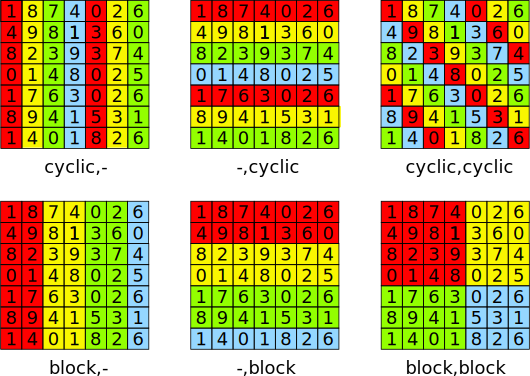
\includegraphics[scale=0.25]{Pics/DISTSTOR1.pdf}
\caption{There are two distinct ways to distribute rows, column or elements along processes, namely cyclic and block. Each color represents a processor (4 in total).}
\label{fig:DISTSTOR1}
\end{figure}

\begin{figure}
\centering
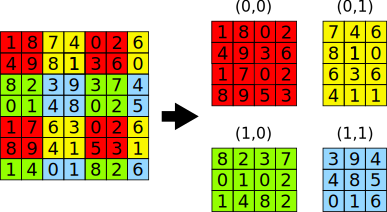
\includegraphics[scale=0.25]{Pics/DISTSTOR2.pdf}
\caption{In the block-cyclic distribution, the matrix is divided into blocks which are distributed over a processor grid, in this case 2 $\times$ 2.}
\label{fig:DISTSTOR2}
\end{figure}

\begin{figure}
\centering
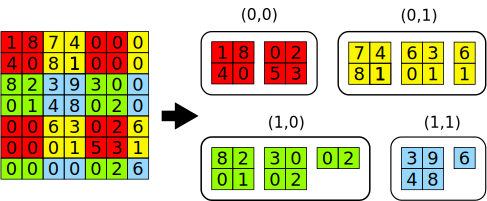
\includegraphics[scale=0.25]{Pics/DISTSTOR3.pdf}
\caption{The DBCSR library distributes the significant blocks over the processor grid in row-major format.}
\label{fig:DISTSTOR3}
\end{figure}

%¨libxsmm?
%The block size has a major impact on the performance of distributed linear algebra algorithms. Consider the multiplication of two matrices. Multiplication can be reformulated in terms of individual multiplications of sub-blocks. 

\section{Tensors}

\subsection{Definitions}

Tensors are multi-dimensional arrays and can be seen as a generalization of matrix objects to higher dimensions, containing a set of complex or real values $\{a_{ijk...}\}$ with the ordered indices $i = 0,1,2,...N_0$, $j = 0,1,2,...N_1$, $k = 0,1,2,...N_2$ etc. The total number of indices required to identify an element in a tensor corresponds to its \emph{dimension}, also called \emph{rank}, \emph{order} or \emph{degree}. It should be stressed that tensor rank is different from the concept of a matrix rank. 

Tensors are important quantities in various scientific fields, especially in physics and quantum chemistry. Examples of tensor are the 4-dimensional MP2-amplitudes $t_{iajb}$ or the 3-dimensional 3c2e electron integrals. Matrices can be seen as 2-dimensional tensors. 

The analog of matrix multiplication is \emph{tensor contraction}, which involves the summation over one or multiple indices. Consider for example the tensor contraction
\begin{equation}
C_{ijm} = \sum_{kl} A_{ikjl} B_{lkm}
\end{equation}
\noindent Here, the summation runs over the indices $kl$. Alternatively, the expression above can be abbreviated as
\begin{equation}
C_{ijm} = A_{ikjl} B_{lkm}
\label{eq:TENEX}
\end{equation}
\noindent which is known as  \emph{Einstein summation}, a notational convention used to simplify tensor expressions. Indices appearing on the right but not on the left are implicitly summed over. 

\subsection{Tensor Storage and Mapping \label{sec:tenstor}}

Mapping multi-dimensional to the linear main memory is non-trivial. Tensors may follow a generalized column or row major storage such that
\begin{align}
A(i_0,i_1,...,i_n) &\rightarrow \sum_{k=0} \left( \prod_{l=k+1}^{N_{dim}} n_l \right) i_k \qquad \textrm{row-major} \\
A(i_0,i_1,...,i_n) &\rightarrow \sum_{k=0} \left( \prod_{l=0}^{k-1} n_l \right) i_k \qquad \textrm{column-major} 
\end{align} 
\noindent where $N_{dim}$ is the dimension of the tensor, and $n_k$ is the size of dimension $k$.

Consider again the tensor contraction \ref{eq:TENEX}. It can be programmed by just looping over all elements explicitly:
\begin{fortran}{Tensor Loop \label{lst:TLOOP}}
DO i = 1, ndim_i
  DO j = 1, ndim_j
    DO m = 1, ndim_m
      DO k = 1, ndim_k
        DO l = 1, ndim_l
          C(i,j,m) = A(i,k,j,l) * B(l,k,m)
        ENDDO
      ENDDO
    ENDDO
  ENDDO
ENDDO
\end{fortran}
\noindent Similarly to Example \ref{FORTRAN1} which loops over matrix elements, efficient parallelization by means of vectorization is a major concern when coding tensor contractions by hand. Ideally, tensor contractions should be offloaded to a specialized library. However, writing a general tensor library is a complex task, as the optimal kernel is dependent on the nature of the tensor contraction, i.e. number of indices involved, tensor dimensions and memory mapping. Whereas the \textrm{dgemm} BLAS routine only needs to know whether the matrices are transposed or not, the rapidly increasing number of parameters and loops makes it very difficult to write optimized code for arbitrary tensor contractions. For the example above, there are already $5!$ = $120$ different ways to arrange the loops.  

Many tensor libraries solve this problem by mapping tensors to matrices so that existing code for optimized matrix-matrix multiplication can be used instead. Consider the tensor $A_{ikjl}$. By introducing the \emph{super-indices} $P$ and $Q$, the tensor can be mapped to a matrix with $N_P$ = $n_i n_k$ rows and $N_Q$ = $n_j n_l$ columns with
\begin{align}
P(i,k) &= i + k*n_i \\
Q(j,l) &= j + l*n_j
\end{align}
\noindent The individual tensor elements are then accessed by
\begin{equation}
A(i,k,j,l) \rightarrow P(i,k) + Q(j,l) N_P
\end{equation}
\noindent using column-major storage for both the indices and super-indices. This corresponds to mapping $ik$ to the rows and $jl$ to the columns of a large matrix, which may also be written in a condensed notation as $\cn{01}{23}$, where $0,1,...$ indicate the mapping of the first, second, ... index of the tensor. As another example, consider the mapping $\cn{0}{213}$: this indicates that the index $i$ is mapped to rows, and $jkl$ are mapped to the columns. Alternatively, the mapping can be indicated by using upper or lower indices. $\cn{01}{23}$ corresponds to $A_{ik}^{jl}$ and $\cn{0}{213}$ to $A_{i}^{jkl}$. The lower indices are also known as \emph{covariant} indices, and the upper indices as \emph{contravariant} indices. From here on out, only the notation $\cn{\cdot}{\cdot}$ will be used.

Coming back to the tensor contraction in \ref{eq:TENEX}, mapping the tensors according to $A_{ikjl}^{\cn{02}{13}}$, $B_{lkm}^{\cn{10}{2}}$ and $C_{ijm}^{\cn{01}{2}}$, the contraction can be reformulated as a simple matrix multiplication
\begin{equation}
\mbf{C} = \mbf{A} \mbf{B}
\end{equation}
\noindent and optimized matrix libraries can be used to perform the tensor contraction. It is also possible to choose the mapping $B_{lkm}^{\cn{2}{10}}$, and the tensor contraction may be expressed as
\begin{equation}
\mbf{C} = \mbf{A} \mbf{B}^T
\end{equation}
\noindent by taking the transpose of $\mbf{B}$. In general, any tensor contraction can be reformulated as a matrix multiplication by mapping the indices which are summed over to either the row or column of a matrix, and the indices which are not involved to the remaining dimension. 

There are two drawbacks to this approach: first, tensors which are participating in different types of tensor contractions may need to be reordered. Reordering can take up a significant amount of time and add overhead to the tensor contraction, and it effectively doubles the amount of space needed by the tensor. Second, standard matrix libraries may not be optimized to handle tall-and-skinny (TAS) matrices. TAS matrices are matrices where one dimension is much larger then the other one, which is often the case for tensors with uneven mappings. Consider the tensor  $B_{lkm}^{\cn{10}{2}}$. It maps to a matrix with $n_kn_l$ rows and $n_m$ columns. If this matrix is distributed over an MPI grid, the process columns have much more work to perform than the process rows, which may lead to load imbalances. This problem can be addressed by dividing the TAS matrices into multiple square submatrices to improve load balancing, but at the cost of adding further complexity to the code.

\section{Matrix Libraries}

This section briefly describes the different matrix libraries that are used in \mchem{}.

\subsection{BLAS}

Basic Linear Algebra Subroutines (BLAS) is a \emph{specification} that describes a set of fundamental operations on vectors and matrices which serve as building blocks for higher level algebraic functionality \cite{BLAS2021}. The subroutines are grouped into different \emph{levels}. BLAS 1 provides vector-vector operations, BLAS 2 performs matrix-vector operations, and BLAS 3 provides matrix-matrix operations. Implementations of the BLAS library are often optimized for a certain type of processor, such as Intel's math kernel library (MKL) or the BLAS-like instantiation software (BLIS) which are optimized for Intel and AMD processors respectively. By providing a general interface, BLAS-based code is highly portable and should be preferred over processor-dependent, intrinsic functions. 

\subsection{LAPACK}

The linear algebra package (LAPACK) provides routines for matrix factorizations such as the QR decomposition, eigenvalue decomposition or singular value decomposition \cite{LAP2021}. It also includes functions for solving systems of linear equations and linear least squares problems. The official Netlib LAPACK implementation is based on BLAS and therefore highly portable, and simply linking the corresponding BLAS library that is optimized for the targeted architecture is sufficient. However, processor-specific re-implementations of LAPACK such as Intel MKL also exist. LAPACK can handle dense matrices only. 

\subsection{Eigen}

Eigen is a C++ template library that provides basic and advanced matrix algebra routines, including numerical solvers and matrix decompositions \cite{Gue2010}. Compared to LAPACK, Eigen offers a more user-friendly interface with an API that is closer in form to to standard algebraic notation. A matrix multiplication with addition is as simple as writing
\begin{cpp}{Eigen Matrix Multiplication}
Eigen::MatrixXd A, B, C;
// initialize matrices
A = A + B * C;
\end{cpp}
\noindent Matrix manipulations, such as row, column or block operations are also much more intuitive, which is its primary use in \mchem{}.

\subsection{PBLAS}

PBLAS (Parallel BLAS) is a generalization of the BLAS specification to distributed memory environments \cite{PBLAS2021}. It uses BLACS (basic linear algebra communication subprograms) as the message passing interface, typically built on MPI, and optimized for 2D grid communication. Matrices and vectors use a block-cyclic distribution with homogeneous block sizes across processor rows and columns. Similarly to BLAS, it provides a general interface and several different implementations exist (Netlib, Intel MKL, IBM, Cray). It closely mimics the function signature of BLAS, but matrices have an additional \emph{array descriptor} which holds all parameters of the matrix distribution. Matrix multiplication is performed using Cannon's algorithm \cite{Can1969}.

\subsection{ScaLAPACK}

Scalable LAPACK (ScaLAPACK) is LAPACK's analog for distributed memory systems \cite{Sca2021}. It provides highly optimized, advanced linear algebra routines based on the PBLAS interface.  It solves linear least squares, eigenvalue and singular value decomposition problems, among others. Again, while the specification is general, processor optimized implementations are often encountered, which are even more crucial in the context of high-performance computing. 

Compared to LAPACK, ScaLAPACK does not support many matrix decompositions with pivoting. Pivoting incurs a very high overhead due to the increased communication between nodes.

\subsection{DBCSR}

DBCSR (distributed block compressed sparse row) is a Fortran library designed for efficient sparse matrix multiplication in distributed memory environments \cite{Bor2014,DBCSR2020}. It is OpenMP and MPI parallel and can exploit NVIDIA and AMD GPUs via Cuda and HIP. It uses a sparse block-cyclic matrix storage format (Figure \ref{fig:DISTSTOR2}) and was originally developed for linear-scaling self-consistent field calculations within CP2K, a quantum chemistry and solid state physics software package \cite{Hut2014,Sch2016}. 

The DBCSR matrix multiplication architecture is divided into several layers managing data transfer, data access and offloading. Figure \ref{fig:ARCH} shows a schematic representation of the layers. The top-most layer manages the parallelization of the matrix multiplication over multiple nodes, and subdivides the matrix into large sparse sub-matrices, or \emph{panels}, which contain approximately the same number of blocks. A block-generalized version of Cannon's algorithm \cite{Can1969} is used to communicate the panels to different processes in a regular and ordered fashion. At each "tick" of Canon's algorithm, each process  sends and receives panels which it then multiplies and adds to the local blocks. 

The multiplication of the panels is handled by the multrec layer, which subdivides panels \emph{recursively} along the longest dimension until the submatrices are small enough to fit into cache size.

The CSR layer then determines which blocks need to be multiplied from the sparsity pattern of the matrices. It generates a list of needed block-multiplications, called \emph{stacks} and passes this information to the scheduler. The scheduler receives the stacks and arranges them for processing by handing them off to different drivers. Stacks can be processed either by the host (CPU) or the device (GPU). Both drivers support standard matrix multiplication by using (cu/hip)-BLAS, as well as small matrix multiplication (SMM) which are handled by specialized SMM libraries optimized for CPU (libxsmm) or GPU (libsmm\_acc). 

For a multiplication of matrices with dimension $N$ by $K$ and $K$ by $M$, a problem size suitable for SMM libraries approximately falls within $(MNK)^{1/3} < 64$. Block-sparse matrices in quantum chemistry often have very small block sizes. However, standard libraries like BLAS are most often optimized for very large matrices, and SMM libraries are often crucial to reduce the overhead when using small block sizes. 

In 2019, the DBCSR library  was extended to handle tensor contractions using the TAS matrix mapping discussed above \cite{Siv2019}. It is an \emph{ad-hoc} extension of the DBCSR matrix machinery, and still somewhat experimental. Memory issues are commonly encountered (see chapter 7).

A C-interface to the DBCSR library was written as part of this PhD project \cite{Amb2020}.

%OTHER POSSIBILTY: https://arxiv.org/abs/1607.00291

\begin{figure}
\centering
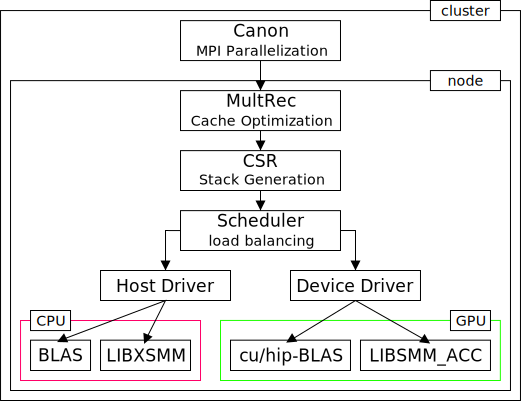
\includegraphics[scale=0.9]{Pics/DBCSRARCH}
\caption{Code architecture of the DBCSR library.}
\label{fig:ARCH}
\end{figure}





\chapter{MEGALOchem: User Guide}

A user guide for MEGALOchem

\chapter{MEGALOchem: Developer Guide}

\section{Software Architecture}

\section{Software Philosophy}

builder functions. named constructors

\section{Modules}

Main. Input, josn, etc...

\subsection{Utils}

\subsection{Extern}

\subsection{dbcsrx}

\subsection{Math}

\subsection{Desc}

\subsection{Ints}

\subsection{Fock}

\subsection{hf}

\subsection{mp}

\subsection{adc}

\subsection{locorb}

\chapter{Algorithms}

The final chapter collects a few of the more important numerical algorithms and solvers used in the \mchem{} software, with some comments on the implementation details.

\section{Direct Inversion of The Iterative Subspace \label{sec:DIIS}}

The direct inversion of the iterative subspace (DIIS) method is an acceleration technique for solvers of nonlinear equations, originally introduced by Pulay \cite{Pul1980} in the context of the self-consistent field method. It has also found use in the solution of  the coupled cluster amplitude equations via Newton-Raphson methods, as well as in the Davidson diagonalization procedure. 

At a given iteration $i$, the DIIS method tries to find a set of coefficients $c_i$ such that the sum of the $m$ previous error vectors 
\begin{equation}
\mbf{e}_{i+1} = \sum_{i=0}^m c_i \mbf{e}_i
\end{equation}
\noindent approximates the null vector in a least-squares sense. The new coefficients are then used to extrapolate the solution $\mbf{p}$ for the next iteration using the current set of solution vectors:
\begin{equation}
\mbf{p}_{i+1} = \sum_{i=0}^m c_i \mbf{p}
\end{equation} 
\noindent In the classical DIIS scheme, the coefficients are furthermore required to sum to one 
\begin{equation}
\sum_i^m c_i = 1
\label{eq:DIIS_CONSTRAINT}
\end{equation}
\noindent Finding the coefficients thus corresponds to minimizing the Lagrangian subject to the constraint \ref{eq:DIIS_CONSTRAINT}:
\begin{equation}
\mathcal{L} = \mbf{c}\pdg \mbf{B} \mbf{c} - \lambda \left( 1 - \sum_i^m c_i \right)
\end{equation}
\noindent where $\mbf{B}$ is the matrix (or \emph{subspace})
containing the overlaps
\begin{equation}
B_{ij} = \sbraket{e_i}{e_j}
\end{equation}
\noindent Minimizing $\mathcal{L}$ with respect to $\mbf{c}$ gives
\begin{equation}
\frac{\partial \mathcal{L}}{\partial c_k} = 2 \sum_i^m c_i B_{ki} - \lambda = 0
\end{equation}
\noindent which then reduces to the matrix equation
\begin{equation}
\begin{pmatrix}
B_{00} & B_{01} & \ldots & B_{0m} & -1 \\
B_{10} & B_{11} & \ldots & B_{1m} & -1 \\
\vdots & \vdots & \ddots & \vdots & \vdots \\
B_{m0} & B_{m1} & \ldots & B_{mm} & -1 \\
-1 & -1 & \ldots & -1 & 0
\end{pmatrix}
\begin{pmatrix}
c_0 \\
c_2 \\
\vdots \\
c_m \\
\lambda 
\end{pmatrix}
=
\begin{pmatrix}
0 \\ 0 \\ \vdots \\ 0 \\ -1
\end{pmatrix}
\end{equation}
\noindent The system can be solved by inverting the subspace matrix (hence the name DIIS). 
The DIIS method is straight-forward to implement. Algorithm \ref{algo:DIIS} gives a summary for the method as it is used in the SCF procedure. 
The exact form of the error vector (or \emph{residual}) depends on the nature of the problem. In the general case, one can use the quantity
\begin{equation}
\mbf{e}_i = \mbf{e}_i - \mbf{e}_{i-1}
\end{equation}
\noindent In the case of the SCF method, the commutator relationship may be used instead:
\begin{equation}
\mbf{e}_i = \mbf{F}_i \mbf{P}_i \mbf{S} - \mbf{S} \mbf{P}_i \mbf{F}_i 
\end{equation}
In some cases, it is beneficial to remove some error vectors from the subspace to avoid linear dependencies. One can either remove the first error vector, or the vector with the largest norm. In most quantum chemistry software packages, the maximum DIIS space is set between 8 and 12. 

\begin{algorithm}
Compute the new Fock matrix $\mbf{F}_i$ for the current iteration $i$ using the density matrix $\mbf{P}_i$
\\
Compute the error vector $\mbf{e}_i = \mbf{F}_i \mbf{P}_i \mbf{S} - \mbf{S} \mbf{P}_i \mbf{F}_i$
\\
Add the error vector $\mbf{e}_i$ and the $\mbf{F}_i$ to the trial vectors. If the number of trial vectors is larger than a given threshold \textrm{DIIS\_MAX\_SUBSPACE}, remove  the first vector in the sets $\{\mbf{F}\}$ and $\{\mbf{e}\}$, or erase entry $k$ where $\mbf{e}_k$ is the error with the largest norm.
\\
Compute the overlap matrix $\mbf{B}$ and minimize the Lagrangian
\\
Compute a new Fock matrix using the new coefficients $\mbf{F}_{i+1} = \sum_i^m c_i \mbf{F}_i$, and diagonalize it to get the new density matrix $\mbf{P}_{i+1}$. 
\\
Increment $i$, begin new cycle
\caption{DIIS method for SCF}
\label{algo:DIIS}
\end{algorithm} 

\section{Davidson Diagonalization \label{sec:DAV}}

Eigenvalue problems involving large, symmetric matrices are ubiquitous in electronic structure theory. Due to the steep scaling in the number of elements, a full diagonalization is often not possible. Fortunately, in most cases the interest lies only in a few select eigenvalues, rather than the whole spectrum, and iterative methods may be used that avoid storing the whole matrix. Davidson's diagonalization procedure \cite{Dav1975} was originally introduced to extract the first few eigenvalues CI matrix, and is mainly used for eigenvalue problems of large, sparse, diagonally dominant matrices. Davidson's method is part of a larger category called \emph{Krylov subspace} methods. Krylov subspaces help to find approximate solutions to a higher-dimensional problem by projecting the matrix onto a smaller subspace that fits in memory. Other methods in this family include the Lanczos and Arnoldi algorithm, which also find uses in quantum chemistry \cite{Cor2012}.

\subsection{Davidson-Liu Method}

The Davidson method builds up an iterative subspace representation of the full matrix which corresponds to the overlap $\sbraket{r_i}{u_j}$ between the current set of trial vectors $\mbf{u}$ and the set of matrix-vector products $\mbf{r} = \mbf{A} \mbf{u}$. Diagonalizing this subspace matrix gives a set of approximate eigenvalues and eigenvectors. New trial vectors are constructed using the preconditioned residual. A \emph{preconditioner} helps to "steer" the problem into the right direction by better approximating the matrix $\mbf{A}$ and thus speeding up convergence. In the original paper, Davidson uses $\mbf{M} = \mbf{D} - \lambda \mbf{I}$ as the preconditioner, where $\mbf{D}$ is the exact diagonal of the matrix. If constructing the diagonal is too expensive, the \emph{Olsen preconditioner} may be used as an alternative, which approximates the diagonal to zeroth order \cite{Ols1990}. For example, the diagonal of the singles-singles block is then simply given by the MO energy differences $D_{ia} = \eps_i - \eps_a$. Other more sophisticated preconditioners have also been investigated \cite{Mor1990}. 

The quality of the starting guess vectors also influences convergence rate. In most quantum chemistry programs, they are constructed by considering the exact or approximate matrix diagonal $\mbf{D}$. The entries of $\mbf{D}$ are ordered from highest to lowest norm. The first guess vector is then generated by putting a 1 on the position of the matrix element with the highest norm, with the rest of the elements set to 0. The second, third, ... eigenvectors are constructed in a similar way. Eigenvectors from a lower order calculation can also be used as a starting guess for higher order methods (e.g. using CIS eigenvectors for ADC(2)). 

The Davidson method was originally a single-root method, i.e. each root needed a separate optimization. A \emph{blocked} version was proposed by Liu \cite{Liu1978}, which allows to optimize multiple roots at once. The blocked Davidson-Liu method as implemented in \mchem{} is given in Algorithm \ref{algo:DAVIDSON}. If only a single root is needed, the loops over the states are restricted to a single index instead, where $i_{root}$ corresponds to the desired root index. 

Furthermore, the Davidson procedure can be modified such that it follows eigenvectors that have a desired structure. The so-called \emph{root-homing} procedure \cite{But1976} reorders the eigenvalues and eigenvectors at each iteration according to overlap criteria. If one wishes to preserve the structure of the initial guesses, root-homing is essential. This modification to the Davidson algorithm is not implemented in \mchem{}.

While the Davidson algorithm avoids storing the whole matrix, it still needs to save the trial vectors and matrix-vector products. As the subspace grows, so does the number of vectors, which might become a memory bottleneck. To limit the number of vectors, the Davidson subspace can be collapsed and a new set of vectors can be formed according to
\begin{equation}
\mbf{u}'_i = \sum_j^{n_{dav}} V_{ji} \mbf{u}_j
\label{eq:COLLAPSE1} 
\end{equation}
\noindent where $\mbf{V}$ are the eigenvectors of the subspace matrix. This is followed by a normalization step
\begin{equation}
\mbf{u}^{new}_i = \frac{\mbf{u}'_i}{\vnorm{\mbf{u'}_i}}
\label{eq:COLLAPSE2}
\end{equation}
\noindent Subspace collapse allows to formulate a better estimate of the total memory requirements of the procedure. 

\begin{algorithm}
\setstretch{1.1}
\KwIn{Number of desired roots $n_{root}$, guess vectors $\mbf{U} = \{ \mbf{u}_i \}$, convergence threshold $d_{conv}$, (approximate) diagonal $\mbf{D}$, matrix-vector product function \textrm{mvp\_func()}}
\KwOut{Converged eigenvectors $\{\mbf{v}_i \}$ and eigenvalues $\{\omega_i \}$}

\While{not converged}{
Compute all the matrix-vector products which have not yet been computed
\begin{equation*}
\mbf{r}_{\oli} = \textrm{mvp\_func}(\mbf{u}_{\oli})
\end{equation*}
\\
Form the subspace matrix 
\begin{equation*}
A_{\oli\olj} = \mbf{r}_{\oli} \cdot \mbf{u}_{\olj} 
\end{equation*}
\\
Diagonalize $\mbf{A}$ to get the eigenvectors $\mbf{V} = \{\mbf{v}_{\oli} \}$ and eigenvalues $\{\omega_{\oli} \}$
\\
Compute the $n_{root}$ residuals 
\begin{equation*}
\boldsymbol{\rho}_i = \mbf{r}_{\olj} V_{\olj i}  - \mbf{u}_{\olj} V_{\olj i} \omega_{i}  
\end{equation*}
\\
Root $i$ has converged if $\vnorm{\boldsymbol{\rho}_i} < d_{conv}$ or $\left\lvert V(n_{dav}-1,i) \right\rvert < d_{conv}$ 
\\
If all roots have converged, then break, else continue.
\\
Compute the correction vectors $\{\mbf{e}_i\}$
\begin{equation*}
\mbf{e}_i = \frac{\boldsymbol{\rho}_i}{\mbf{D} - \omega_i \mbf{I}}
\end{equation*}
\\
Compute a new set of vectors $\{\mbf{b}_i\}$ by Gram-Schmidt orthogonalization of $\{\mbf{d}_i\}$ against the current set of $\{\mbf{u}_{\oli}\}$ 
\\
Normalize the new vectors $\{\mbf{b}_i\}$ and add all vectors to $\{\mbf{u}_{\oli}\}$ for which $\vnorm{\mbf{b}_i}/\vnorm{\mbf{d}_i}$ are above 1e-3 (to remove linear dependencies)
\\
If the size of the Davidson subspace $n_{dav}$ is above a given threshold, collapse the subspace and form a new set according to Equations \ref{eq:COLLAPSE1} and \ref{eq:COLLAPSE2}
} % end while

The final eigenvalues are equal to the eigenvalues of the last subspace matrix. The final eigenvectors $\{\mbf{v}_i\}$ are formed according to Equations \ref{eq:COLLAPSE1} and \ref{eq:COLLAPSE2} using the trial vectors $\{\mbf{u}_i\}$ and the eigenvectors of the subspace matrix 

\caption{Davidson-Liu Algorithm. Indices $i,j,k...$ implicitly loop over the number of roots $n_{roots}$, and indices $\oli, \olj, \olk, ...$ implicitly loop over the whole Davidson subspace $n_{dav}$.}
\label{algo:DAVIDSON}
\end{algorithm}

\subsection{Modified Davidson Method for the Pseudo-Eigenvalue Problem}

When using doubles-folding in the context of the ADC(2) or CC2 method (section \ref{sec:ADC_DAV}), the effective matrix $\mbf{A}_{eff}$ becomes dependent on its own eigenvalues:
\begin{equation}
\mbf{A}_{eff}(\omega) \mbf{v} = \omega \mbf{v}
\end{equation}
\noindent In this case, the standard Davidson method does not work, and needs to be modified to be able to solve this pseudo-eigenvalue problem. Different approaches have been proposed over the years, but are each based on similar principles \cite{Kat2009,Win2011}. The modified Davidson algorithm is given in Algorithm \ref{algo:PSEUDODAVIDSON}, as implemented in \mchem{}. 

The algorithm is split into \emph{macro} and \emph{micro} iterations, which are state-specific. The micro-iterations corresponds to the standard single-root Davidson iterations for diagonalizing an effective matrix $\mbf{A}_{eff}(\omega_i)$ with \emph{fixed} eigenvalue $\omega_i$. When the procedure has converged, $\omega_i$ is set to the new eigenvalue $\omega_i'$, and a new Davidson procedure, or macro-iteration commences with the effective matrix $\mbf{A}_{eff}(\omega_i)$. The macro-iterations are repeated until the eigenvectors have converged to a certain threshold. The individual roots are then further converged using DIIS.

\begin{algorithm}
\setstretch{1.1}
\KwIn{Number of desired roots $n_{root}$, guess vectors $\{ \mbf{u}_i \}$ and eigenvalues $\{ \omega^{(0)}_i \}$, convergence threshold $d_{conv}$, (approximate) diagonal $\mbf{D}$, matrix-vector product function \texttt{mvp\_func()}}
\KwOut{Converged eigenvectors $\{\mbf{v}_i \}$ and eigenvalues $\{\omega_i \}$}
Set $\omega^{macro}_i$ to $\omega^{(0)}_i$ and start macro-iterations for each individual state $i$
\\
\While{not converged}{
	Perform Davidson diagonalization on the effective matrix $\mbf{A}(\omega^{macro}_i)$. Convergence is reached when the difference between eigenvalues $\omega^{micro}_i$ from subsequent micro-iterations is smaller than the total change since the start of the procedure, i.e. at iteration $n$:
\begin{equation*}
\texttt{abs} \left( \omega^{macro}_i - \omega^{micro}_i \vert_{\textrm{iter} = 0} \right) > \texttt{abs} \left( \omega^{micro}_i \vert_{\textrm{iter}=n} - \omega^{micro}_i \vert_{\textrm{iter}=n-1} \right)  
\end{equation*}
\\
If the residual $\boldsymbol{\rho}_i$ is smaller than 1e-3, break, else continue
\\
Set $\omega^{macro}_i$ to $\omega^{micro}_i$, and $\mbf{u}_i$ to $\mbf{v}^{micro}_i$
} % end while
Set $\omega_i$ to $\omega^{macro}_i$, start DIIS
\\
\While{not converged}{
	Compute the matrix-vector product $\mbf{r}_i = \texttt{mvp\_prod}(\mbf{u}_i,\omega_i)$
	\\
	Compute the residual
	\begin{equation*}
	\boldsymbol{\rho}_i = \frac{\mbf{r}_i - \omega_i \mbf{u}_i}{\vnorm{\mbf{u}_i}}
	\end{equation*}	 
	\\
	Compute the new eigenvalue $\omega_i$
	\begin{equation*}
	\omega_i = \frac{\mbf{u}_i \cdot \mbf{r}_i}{\vnorm{\mbf{u}_i}}
	\end{equation*}
	\\
	If $\vnorm{\boldsymbol{\rho}_i} < d_{conv}$, root $i$ has converged, break
	\\
	Compute the corrected vector $\mbf{b}_i$ according to
	\begin{equation*}	 
	\mbf{b}_i = \mbf{u}_i + \frac{\boldsymbol{\rho}_i}{\mbf{D}}
	\end{equation*} 
	\\
	Add $\boldsymbol{\rho}_i$ to the DIIS error vector space, and perform extrapolation on $\boldsymbol{b}_i$ to get a new guess vector $\mbf{u}_i$ 
} % end while

\caption{Modified Davidson algorithm with DIIS acceleration for pseudo-eigenvalue problems.}
\label{algo:PSEUDODAVIDSON}
\end{algorithm}

%\section{Boys Localization \label{sec:LOCORB}}

\section{Incomplete Cholesky Decomposition \label{sec:CHOLDEC}}

The Cholesky factorization decomposes a symmetric, positive definite (PD) matrix into a lower and upper triangular matrix:
\begin{equation}
\mbf{A} = \mbf{L} \mbf{L}^T
\label{eq:NONPIVCHOL}
\end{equation}
\noindent where $\mbf{L}$ has the same dimension as $\mbf{A}$. However, the Cholesky factorization, as defined in \ref{eq:NONPIVCHOL}, does not exist for positive semi-definite (PSD) matrices. To see the reason why, consider Algorithm \ref{algo:CHOL} for the standard Cholesky factorization. The loop runs over all columns $i$ of $\mbf{A}$  and involves divisions by the diagonal elements $L_{ii}$. For PSD matrices, some of these elements will be zero due to linear dependencies of the column vectors, and the operation is therefore not defined.

\begin{algorithm}
\setstretch{1.1}
\KwIn{Symmetric matrix $\mbf{A}$ with dimension $N$ by $N$}
\KwOut{Cholesky factors $\mbf{L}$}
$L_{00} \leftarrow \sqrt{A_{00}}$
\\
$L_{j0} \leftarrow \frac{a_{j0}}{L_{00}} \quad j \in [1:N]$
\\
$L_{ii} \leftarrow \sqrt{ A_{ii} - \sum_{k=0}^{i} L_{ik}^2} \quad i \in [1:N]$ 
\\
$L_{ji} \leftarrow \left( A_{ji} - \sum_{k=0}^{i} L_{ik} L_{jk} \right) / L_{ii} \quad i \in [1:N] \quad j \in [i+1:N]$
\caption{Cholesky decomposition without pivoting.}
\label{algo:CHOL}
\end{algorithm}
 
A PSD matrix is also called \emph{rank-deficient}. The rank of a symmetric matrix is equal to the number of linearly independent column vectors. The occupied atomic density matrix $\mbf{P}$ is an example of a rank-deficient matrix. The atomic orbital basis, with $N_{bas}$ functions, is often redundant and has linear dependencies, which translates to a lower rank $r < N_{bas}$ of the occupied density matrix. The rank of $\mbf{P}$ is equal to the number of occupied molecular orbitals. The atomic orbital overlap matrix $\mbf{S}$ is an example of a "numerically" positive semi-definite matrix. While the column vectors are not strictly linearly dependent from a mathematical point of view, they are linearly dependent in the sense of floating-point precision. The diagonals $L_{ii}$ are close to zero ($<$ 1e-5), which will lead to large values and reduced accuracy when dividing.  

The Cholesky factorization can be generalized to PSD matrices by introducing permutation matrices which pivot the columns and rows of $\mbf{A}$:
\begin{equation}
\mbf{P} \mbf{A} \mbf{P}^T = \mbf{L} \mbf{L}^T 
\end{equation}
\noindent or
\begin{equation}
\mbf{A} = \mbf{P}^T \mbf{L} \mbf{L}^T \mbf{P}
\end{equation}
\noindent where $\mbf{L}$ is a $N$ by $k$ lower triangular matrix with $k = rank(\mbf{A})$. The 
permutation matrices swap the diagonal entries $L_{ii}$, also known as \emph{pivots}, in a way that division by zero is avoided during the procedure. If the pivot is below a certain threshold, the procedure halts and the number of total iterations is equal to the rank of $\mbf{A}$. The \emph{incomplete} pivoted Cholesky factorization is therefore \emph{rank-revealing}. Other examples of rank-revealing decompositions include the pivoted QR decomposition, and the singular value decomposition.

The Cholesky decomposition with full pivoting is given in Algorithm \ref{algo:CHOLPIV}. It can also be used in cases where the matrix is nearly positive semi-definite ($N \approx rank(A)$) for extra numerical stability, e.g. the AO overlap matrix. In \mchem{}, the pivoted Cholesky factorization is used to obtain a set of localized Cholesky MO coefficients which help to reduce the prefactor of atomic orbital methods. 

\begin{algorithm}
\setstretch{1.1}
\KwIn{Symmetric matrix $\mbf{A}$ with dimension $N$ by $N$, threshold $d_{lindep}$}
\KwOut{Cholesky factors $\mbf{L}$ and the rank $r$ of $\mbf{A}$}
Initialize index vector $perm = \{0,1,2,...,N\}$
\\
\For{$i = 0$ \textbf{to} $N$}{
	Find maximum diagonal element $A_{max} = A_{jj}$
	\\
	Swap rows $i$ and $j$ of $\mbf{A}$
	\\
	Swap columns $i$ and $j$ of $\mbf{A}$
	\\
	Swap $perm(i)$ and $perm(j)$
	\\
	\uIf{$A_{max} < 0$}{
		Negative pivot element, the Cholesky decomposition is not possible
	} 
	\uIf{$abs(A_{max}) < d_{lindep}$}{
		$r = i+1$, break
	}
	$L_{ii} = \sqrt{A_{max}}$
	\\
	$L_{ki} =  A_{ki}/\sqrt{A_{max}} \quad k \in [i+1:N]$
	\\
	$A_{kl} = A_{kl} - L_{ki} L_{kl} \quad k,l \in [i+1:N]$
} % endfor 
Impose original order of the rows, set row $perm(i)$ of the new Cholesky matrix $\mbf{L}'$ to row $i$ of $\mbf{L} \quad i \in [0:r]$
\\
Set $\mbf{L}$ to $\mbf{L}'$

\caption{Incomplete Cholesky decomposition with full pivoting.}
\label{algo:CHOLPIV}
\end{algorithm}

\subsubsection{Comments}

It should be noted that pivoting destroys the banded structure of the matrix $\mbf{L}$ (Figure \ref{fig:LOCORB_CHOL}). In other words, the pivoted Cholesky factorization of a diagonally dominant, sparse matrix may not give sparse matrices $\mbf{L}$ in the block-diagonal form. Blocking significant elements together reduces the number of non-zero blocks, which is crucial for the performance of atomic orbital based methods. It is therefore necessary to reorder the columns of $\mbf{P^TL}$ at the end of the procedure. In \mchem{}, this is done by sorting the columns by their weight $n = (p_f - p_i) / 2$, where $p_i$ is the first significant element in the column, and $p_f$ is the last significant element. The block-diagonal form can then restored for $\mbf{L}$. 

The pivoted Cholesky decomposition in \mchem{} does not exploit sparsity and scales with $\mathcal{O}(N^2rank(A))$. While a sparse implementation could be considered, row and column pivoting often destroys sparsity patterns (also known as \emph{fill-in}) and leads to a lot of reordering within the sparse data structures. Pivoting needs to be applied in such a way that fill-in is reduced to keep scaling low. 

Finally, pivoting also negatively impacts parallelization when using MPI. When columns are swapped, this incurs additional communication overhead between processes. Moreover, global communication is necessary to communicate the position and value of the maximum diagonal element to each process, which further slows down the procedure. Efficient parallelization of matrix decompositions with pivoting is subject of current research \cite{Xia2016,Xia2017}.

\section{Laplace Transformation \label{sec:LAPLACE}}

The Laplace transformation is  a crucial step for formulating an orbital invariant MP2 energy expression, where the orbital energy denominator is converted to an exponential form 
\begin{equation}
\frac{1}{\eps_a + \eps_b - \eps_i - \eps_j } = \frac{1}{x} = \int_0^{\infty} e^{-xt} dt
\end{equation} 
\noindent The integral is then approximated by the Laplace quadrature
\begin{equation}
\frac{1}{x} = \sum_{\alpha = 0}^{k} \omega\pa e^{-xt\pa}  
\end{equation}
\noindent where $k$ is the number of quadrature points, $\omega\pa$ are the Laplace weights and $t\pa$ are the Laplace exponents. In their original paper, Häser and Almlöf \cite{Has1992} computed the Laplace parameters by least-squares minimization of the error distribution function
\begin{equation}
\eta_k (x,\omega\pa,t\pa) = \sum_{\alpha = 0}^k \omega\pa e^{-xt\pa} - \frac{1}{x}
\end{equation}
\noindent in the interval $[x_{min},x_{max}]$. Later, it was shown that the quadrature parameters can be computed at a much lower cost using a minimax approximation (MA) \cite{Tak2008}, which \emph{minimizes} the \emph{maximum} Chebychev norm
\begin{equation}
\delta_{k[1,R]}(\bar{\omega}\pa,\bar{t}\pa) = \max_{x \in [1,R]} \left\lvert \eta_k (x,\bar{\omega}\pa,\bar{t}\pa ) \right\rvert 
\end{equation}
\noindent with the scaled Laplace parameters $\bar{\omega} = \omega x_{min}$, $\bar{t} = t x_{min}$  in the new interval $[1,R]$ where $R = x_{max}/x_{min}$. The scaled Laplace coefficients in the minimax approximation are obtained by repeating the following two steps until self-consistency is reached:
\begin{enumerate}
\item Determine the $2k-1$ extremum points $x_i$ of the error distribution function \\ 
$\eta_k (x,\bar{\omega}\pa,\bar{t}\pa)$ with the current set of $\{\bar{\omega}\}$ and $\{\bar{t}\pa\}$
\item Optimize the $2k+1$ parameters $\{\bar{\omega}\pa\}$ and $\{\bar{t}\pa\}$ by solving the $2k+1$ non-linear equations
\begin{equation}
\eta_k (x_i,\bar{\omega}\pa,\bar{t}\pa) = (-1)^i \delta_{k[1,R]}(\bar{\omega}\pa,\bar{t}\pa)
\end{equation} 
\end{enumerate}
\noindent This procedure is also known as the Remez algorithm (RA). Each of the two steps are non-trivial to compute. The set of non-linear equations in step 2 can be solved by performing a Newton-Raphson minimization using pre-tabulated values of $\{\bar{\omega}\pa\}$ and $\{\bar{t}\pa\}$ as guesses for the first RA iteration. Step 1 is a bit more complicated, and is either solved (a) by first finding the nodal points $x_0$ of the error distribution function to compute the extremum points using Newton-Raphson \cite{Tak2008}, or (b) by finding the extremum points directly using the Newton-Maehly algorithm \cite{Hel2016}. For further details, the reader is referred to the original publications.

All calculations in this report use the robust minimax approximation as proposed by Helmich-Paris and Visscher \cite{Hel2016}. They have published their source code on GitHub (GitHub.com/bhelmichparis/laplace-minimax), which was in turn incorporated into the \mchem{} software.

\section{Cuthill-McKee}

The Cuthill-McKee (CM) algorithm finds a permutation $P$ of a sparse, symmetric matrix that minimizes its \emph{bandwidth} \cite{Cut1969}. A banded matrix is a matrix that has all significant elements clustered around the main diagonal. The bandwidth $k$ is defined as the smallest positive index for which
\begin{equation}
\min_k \left\lvert A(k,k) \right\rvert = 0 \qquad k \in [0,N]
\end{equation}
\noindent The CM algorithm reduces the bandwidth of a matrix by reordering the nodes of the corresponding adjacency or connectivity matrix $\mbf{C}$ (Algorithm \ref{algo:CM}). For a $N$-by-$N$ matrix, there are $N$ nodes. Node $i$ and $j$ are connected if the entry $(i,j)$ of the connectivity matrix is 1, and not connected if the entry is 0. Here, the \emph{degree} of a node is defined by the total number of connections, i.e. the row or column sum
\begin{equation}
degree(i) = \sum_j^N C(i,j)
\end{equation}
In the context of quantum chemistry, the nodes correspond to atoms in a molecule, and the connections to bonds. Reordering the indexing of the atoms based on the connectivity matrix of a molecule allows to significantly reduce the number of blocks needed to store quantities like the overlap matrix, density matrix or 2-electron repulsion integrals when using block-sparse matrix algebra by grouping close atoms together. Figure \ref{fig:RCM} shows how the connectivity matrix is reordered for the FW144 system using the reverse CM algorithm. Two atoms are "connected", if their are within 5 $a_0$ of each other.

\begin{figure}
\centering
\begin{minipage}{0.45\textwidth}
\centering
\includegraphics[width=\textwidth]{Pics/FW144_UNORDERED}
\end{minipage}
\begin{minipage}{0.45\textwidth}
\centering
\includegraphics[width=\textwidth]{Pics/FW144_ORDERED}
\end{minipage}
\caption[Illustration of the Cuthill-McKee algorithm]{Connectivity matrix of FW144 before reordering (left), and connectivity matrix after applying the reverse Cuthill-McKee algorithm (right). Reducing the bandwidth allows to compress matrices and tensors in the AO basis into a much smaller space when using the block-sparse format.}
\label{fig:RCM}
\end{figure}

\begin{algorithm}
\setstretch{1.1}
\KwIn{Sparse symmetric matrix $\mbf{A}$ with dimension $N$ by $N$}
\KwOut{Reordered matrix $\mbf{A}$ with minimized bandwidth.}

Form the binary connectivity matrix $\mbf{C}$ of the input matrix
\\
Instantiate empty queue $Q$ and result array $R$
\\
\While{true} {
	Find node $p$ with minimum degree that is not yet in $R$, and put it into $R$
	\\
	Add all nodes to the queue that are connected to $p$
	\\
	\While{length of $Q \neq 0$}{
		Get fist node $q$ in queue, and pop it from queue
		\\
		\uIf{$q$ in $R$}{
		 	skip to next loop
		}
		\Else{
			add $q$ to $R$
		}
		Append all nodes connected to $q$ not yet in $R$ both to $R$ and $Q$
	} % end while q
	\uIf{size of $R = N$}{
		break
	}
} % end while R
Reorder the rows and columns of $\mbf{A}$ according to $R$ (standard Cuthill-McKee) or the reverse order of $R$ (reverse Cuthill-McKee)

\caption{(Reverse) Cuthill-McKee algorithm.}
\label{algo:CM}
\end{algorithm}

%\section{Quasi-Robust Density Fitting}



\chapter{Conclusion and Outlook}

\chapter{Annex}

Everything else
- second qunatization
- DIIS 
- RCM
- overlap matrix orthogonalization
- SAD (SADNO, SAD...)
- Davidson ? 
- ERI deomposition: cholesky, THC, pseudo-spectral
% cholesky https://link.springer.com/article/10.1007/s00214-009-0608-y
- The evil matrix inversion: considerations
% see https://www.johndcook.com/blog/2010/01/19/dont-invert-that-matrix/ 
% also https://epubs.siam.org/doi/abs/10.1137/1.9780898718027.ch14
- mulliken, boughton pulay
- Basis set overcompleteness

%OTHER: \url{https://www.kth.se/blogs/pdc/2018/11/scalability-strong-and-weak-scaling/}
{\footnotesize
\bibliographystyle{unsrt}
\bibliography{ref}
}

\end{document}